\section{PLANIFICACIÓN DEL PROYECTO}
En este apartado se abordará la planificación inicial del proyecto, detallando los aspectos más relevantes del mismo. 
Se incluirá la identificación de interesados, las tareas a realizar, la estructura de desglose de trabajo, la planificación temporal, los riesgos identificados y el presupuesto inicial.

\subsection{Identificación de Interesados}
Los interesados en el proyecto son las personas o grupos que pueden afectar o verse afectados por el proyecto. 
En el caso de este proyecto, los interesados son los siguientes:
\begin{itemize}
    \item \textbf{Usuarios:} Compradores de sobres, vendedores en subastas, pujadores y coleccionistas. Su satisfacción y experiencia de usuario son críticas para el éxito de la plataforma.
    \item \textbf{Desarrolladores:} Equipo encargado del desarrollo, mantenimiento y actualización de la plataforma.
    \item \textbf{Propietarios/Creadores:} Fundadores y administradores del proyecto, responsables de la visión, dirección y toma de decisiones estratégicas.
    \item \textbf{Inversores:} Personas o entidades que financian el proyecto, con expectativas de retorno sobre su inversión. Su interés reside en la rentabilidad y sostenibilidad del negocio.
    \item \textbf{Proveedores:} Proveedores de servicios tecnológicos y de infraestructura, como \textit{hosting}, sistemas de pago y seguridad.
    \item \textbf{Comunidades:} Grupos y foros de fans y coleccionistas de Pokémon que pueden influir en la popularidad y adopción de la plataforma. Su participación y \textit{feedback} pueden guiar mejoras y nuevas características.
    \item \textbf{Reguladores:} Entidades gubernamentales y de la industria que aseguran el cumplimiento de leyes y regulaciones aplicables al comercio digital y la protección de datos.
\end{itemize}


\subsection{OBS y PBS}
El OBS, \textit{Organizational Breakdown Structure} es una estructura que representa las responsabilidades sobre la realización de las tareas del proyecto. 
Por otro lado, el PBS  \textit{(Product Breakdown Structure)} es una estructura jerárquica que descompone el proyecto en los productos que se deben entregar para cumplir con los objetivos del proyecto.

\subsubsection{OBS} \label{sec:5-OBS}
\hypertarget{sec:5-OBS}{}
En este proyecto, se simulará una pequeña empresa ficticia para su realización. 
Se han identificado los distintos perfiles que intervienen en el proyecto, así como las tareas que cada uno debe realizar. 
Aunque el proyecto se llevará a cabo de forma individual, se ha considerado necesario estructurar estos roles para poder asignar un presupuesto adecuado a cada función.

Los roles identificados se especifican en \coloredUnderline{\hyperlink{table:obs}{Tabla: \ref*{table:obs} \nameref*{table:obs}}}. 
Cabe destacar que el rol de Jefe de Proyecto (JP) es el encargado de supervisar y coordinar el trabajo de los demás roles y este rol ha sido considerado tanto para el alumno como para el tutor del TFG.


\begin{table}[H]
\centering
\hypertarget{table:obs}{}
\caption{OBS (Organizational Breakdown Structure)}
\label{table:obs}
\begin{tabular}{>{\columncolor{lightgreen!20}}p{7cm} p{10cm}}
\toprule
\rowcolor{darkgreen!50}
\textbf{Abreviatura} & \textbf{Rol} \\
\midrule
JP & Jefe de Proyecto \\
\midrule
AN & Analista junior\\
\midrule
DI & Diseñador junior \\
\midrule
DS & Desarrollador de Software junior\\
\midrule
TE & Tester junior \\
\midrule
DOC & Documentador técnico \\
\bottomrule
\end{tabular}
\end{table}
 
Se ha decidido realizar una matriz de asignación de responsabilidades RACI para relacionar las tareas identifcadas en \coloredUnderline{\hyperlink{sec:5-WBS}{\ref*{sec:5-WBS} \nameref*{sec:5-WBS}}} con cada rol.
En esta matriz, a cada tarea se le asigna un rol con una de las siguientes responsabilidades:
\begin{itemize}
    \item \textbf{R:} Responsable. Persona que realiza la tarea.
    \item \textbf{A:} Aprobador. Persona que aprueba la tarea.
    \item \textbf{C:} Consultado. Persona a la que se consulta sobre la tarea.
    \item \textbf{I:} Informado. Persona a la que se informa sobre el avance y los resultados de la tarea.
\end{itemize}
Un mismo recursos puede tener varias responsabilidades en una misma tarea, en tal caso se anotarán separadas por el caracter \textit{``/''}.

\subsubsubsection{Análisis del proyecto}
En la \coloredUnderline{\hyperlink{table:matriz-analisis}{Tabla: \ref*{table:matriz-analisis} \nameref*{table:matriz-analisis}}} se muestra la matriz de responsabilidades para la fase de análisis.
\begin{table}[H]
    \centering
    \caption{Matriz RACI. Análisis del proyecto}
    \label{table:matriz-analisis}
    \hypertarget{table:matriz-analisis}{}
    \begin{tabular}{
    >{\columncolor{lightgreen!20}}m{7cm} 
    >{\columncolor{white}}m{1cm} 
    >{\columncolor{white}}m{1cm} 
    >{\columncolor{white}}m{1cm} 
    >{\columncolor{white}}m{1cm} 
    >{\columncolor{white}}m{1cm} 
    >{\columncolor{white}}m{1cm}}
    \cmidrule(l){2-7}
    \rowcolor{darkgreen!50}
    \cellcolor{white} & \multicolumn{6}{c}{\textbf{Roles}} \\
    \midrule
    \rowcolor{lightgreen!20}
    \cellcolor{darkgreen!50}\textbf{Tarea} & \textbf{JP} & \textbf{AN} & \textbf{DI} & \textbf{DS} & \textbf{TE} & \textbf{DOC} \\
    \midrule
    Análisis del sistema & A & R &  & C &  &  \\
    \midrule
    Análisis de la arquitectura & A & R &  & C &  &  \\
    \midrule
    Análisis de la infraestructura & A & R &  & C &  &  \\
    \midrule
    Determinación del alcance de desarrollo & A & R & I & C & I & I \\
    \bottomrule
    \end{tabular}
\end{table}

\subsubsubsection{Seguimiento del proyecto}
En la \coloredUnderline{\hyperlink{table:matriz-seguimiento}{Tabla: \ref*{table:matriz-seguimiento} \nameref*{table:matriz-seguimiento}}} se muestra la matriz de responsabilidades para la fase de seguimiento.
\begin{table}[H]
    \centering
    \caption{Matriz RACI. Seguimiento del proyecto}
    \label{table:matriz-seguimiento}
    \hypertarget{table:matriz-seguimiento}{}
    \begin{tabular}{
    >{\columncolor{lightgreen!20}}m{7cm} 
    >{\columncolor{white}}m{1cm} 
    >{\columncolor{white}}m{1cm} 
    >{\columncolor{white}}m{1cm} 
    >{\columncolor{white}}m{1cm} 
    >{\columncolor{white}}m{1cm} 
    >{\columncolor{white}}m{1cm}}
    \cmidrule(l){2-7}
    \rowcolor{darkgreen!50}
    \cellcolor{white} & \multicolumn{6}{c}{\textbf{Roles}} \\
    \midrule
    \rowcolor{lightgreen!20}
    \cellcolor{darkgreen!50}\textbf{Tarea} & \textbf{JP} & \textbf{AN} & \textbf{DI} & \textbf{DS} & \textbf{TE} & \textbf{DOC} \\
    \midrule
    Reunión de arranque & A & I & I & I & I & R \\
    \midrule
    Reuniones periódicas & A & I & I & I & I & R\\
    \midrule
    Reunión de revisión & A & I & I & C & I & R  \\
    \midrule
    Reunión final & A & I & I & C & I & R  \\
    \bottomrule
    \end{tabular}
\end{table}

\subsubsubsection{Diseño del sistema}
En la \coloredUnderline{\hyperlink{table:matriz-diseno}{Tabla: \ref*{table:matriz-diseno} \nameref*{table:matriz-diseno}}} se presenta la matriz de responsabilidades correspondiente a la fase de diseño. 
Las tareas listadas en esta matriz son las tareas "hoja" de dicha fase, es decir, aquellas que no se descomponen en subtareas más pequeñas y, por lo tanto, representan las tareas finales 
de la fase de diseño.
\begin{table}[H]
    \centering
    \caption{Matriz RACI. Diseño del sistema}
    \label{table:matriz-diseno}
    \hypertarget{table:matriz-diseno}{}
    \begin{tabular}{
    >{\columncolor{lightgreen!20}}m{7cm} 
    >{\columncolor{white}}m{1cm} 
    >{\columncolor{white}}m{1cm} 
    >{\columncolor{white}}m{1cm} 
    >{\columncolor{white}}m{1cm} 
    >{\columncolor{white}}m{1cm} 
    >{\columncolor{white}}m{1cm}}
    \cmidrule(l){2-7}
    \rowcolor{darkgreen!50}
    \cellcolor{white} & \multicolumn{6}{c}{\textbf{Roles}} \\
    \midrule
    \rowcolor{lightgreen!20}
    \cellcolor{darkgreen!50}\textbf{Tarea} & \textbf{JP} & \textbf{AN} & \textbf{DI} & \textbf{DS} & \textbf{TE} & \textbf{DOC} \\
    \midrule
    \textit{Backend}. Diseño del módulo de usuarios & A &  & I & R &  &  I \\
    \midrule
    \textit{Backend}. Diseño del módulo de cartas & A &  & I & R &  & I \\
    \midrule
    \textit{Backend}. Diseño del módulo de sobres de cartas & A &  & I & R &  & I \\
    \midrule
    \textit{Backend}. Diseño del módulo de subastas & A &  & I & R &  & I \\
    \midrule
    \textit{Backend}. Diseño del módulo de transacciones & A &  & I & R &  & I \\
    \midrule
    \textit{Frontend}. Diseño de logo de la aplicación & A &  & R & I &  & I \\
    \midrule
    \textit{Frontend}. Diseño de la moneda de la aplicación & A &  & R & I &  & I \\
    \midrule
    \textit{Frontend}. Diseño de la temática & A &  & R & C/I &  & I \\
    \midrule
    \textit{Frontend}. Diseño del árbol de navegación & A &  & R & C/I &  & I \\
    \midrule
    \textit{Frontend}. Diseño de las páginas de información & A &  & R & C/I &  & I \\
    \midrule
    \textit{Frontend}. Diseño de las página \textit{Home} & A &  & R & C/I &  & I \\
    \midrule
    \textit{Frontend}. Diseño de las página de error & A &  & R & C/I &  & I \\
    \bottomrule
    \end{tabular}
\end{table}

\subsubsubsection{Implementación del sistema}
En la \coloredUnderline{\hyperlink{table:matriz-implementacion}{Tabla: \ref*{table:matriz-implementacion} \nameref*{table:matriz-implementacion}}} se muestra la matriz de responsabilidades para la fase de implementación.
\begin{table}[H]
    \centering
    \caption{Matriz RACI. Implementación del proyecto}
    \label{table:matriz-implementacion}
    \hypertarget{table:matriz-implementacion}{}
    \begin{tabular}{
    >{\columncolor{lightgreen!20}}m{7cm} 
    >{\columncolor{white}}m{1cm} 
    >{\columncolor{white}}m{1cm} 
    >{\columncolor{white}}m{1cm} 
    >{\columncolor{white}}m{1cm} 
    >{\columncolor{white}}m{1cm} 
    >{\columncolor{white}}m{1cm}}
    \cmidrule(l){2-7}
    \rowcolor{darkgreen!50}
    \cellcolor{white} & \multicolumn{6}{c}{\textbf{Roles}} \\
    \midrule
    \rowcolor{lightgreen!20}
    \cellcolor{darkgreen!50}\textbf{Tarea} & \textbf{JP} & \textbf{AN} & \textbf{DI} & \textbf{DS} & \textbf{TE} & \textbf{DOC} \\
    \midrule
    Reunión de arranque & A & I & I & I & I & R \\
    \midrule
    Reuniones periódicas & A & I & I & I & I & R\\
    \midrule
    Reunión de revisión & A & I & I & C & I & R  \\
    \midrule
    Reunión final & A & I & I & C & I & R  \\
    \bottomrule
    \end{tabular}
\end{table}

\subsubsection{PBS} \label{sec:5-PBS}
\hypertarget{sec:5-PBS}{}
El PBS, \textit{Product Breakdown Structure}, es una estructura jerárquica que descompone el proyecto en los productos que se deben entregar para cumplir 
con los objetivos del proyecto. 
En las siguientes secciones se detallan los productos que se deben entregar en el proyecto BidMon Universe.

\subsubsection{PBS. Visión general}
En la \coloredUnderline{\hyperlink{fig:5_PBS-Vision-General}{Figura \ref*{fig:5_PBS-Vision-General}: \nameref*{fig:5_PBS-Vision-General}}} se muestran los productos de alto nivel que se deben entregar en el proyecto BidMon Universe. 
En las siguientes secciones, se entrará en detalle en cada uno de los productos.

\begin{figure}[H]
    \hypertarget{fig:5_PBS-Vision-General}{}
    \centering
    \includegraphics[width=0.5\linewidth]{figures/5-PBS/5_PBS-Vision-General.png}
    \caption{PBS. Visión general}
    \label{fig:5_PBS-Vision-General}
\end{figure}


\subsubsection{PBS. Análisis del sistema}
En la \coloredUnderline{\hyperlink{fig:5_PBS-Analisis-Sistema}{Figura \ref*{fig:5_PBS-Analisis-Sistema}: \nameref*{fig:5_PBS-Analisis-Sistema}}}, se detallan los productos que se deben entregar en la fase de análisis del sistema.
\begin{figure}[H]
    \hypertarget{fig:5_PBS-Analisis-Sistema}{}
    \centering
    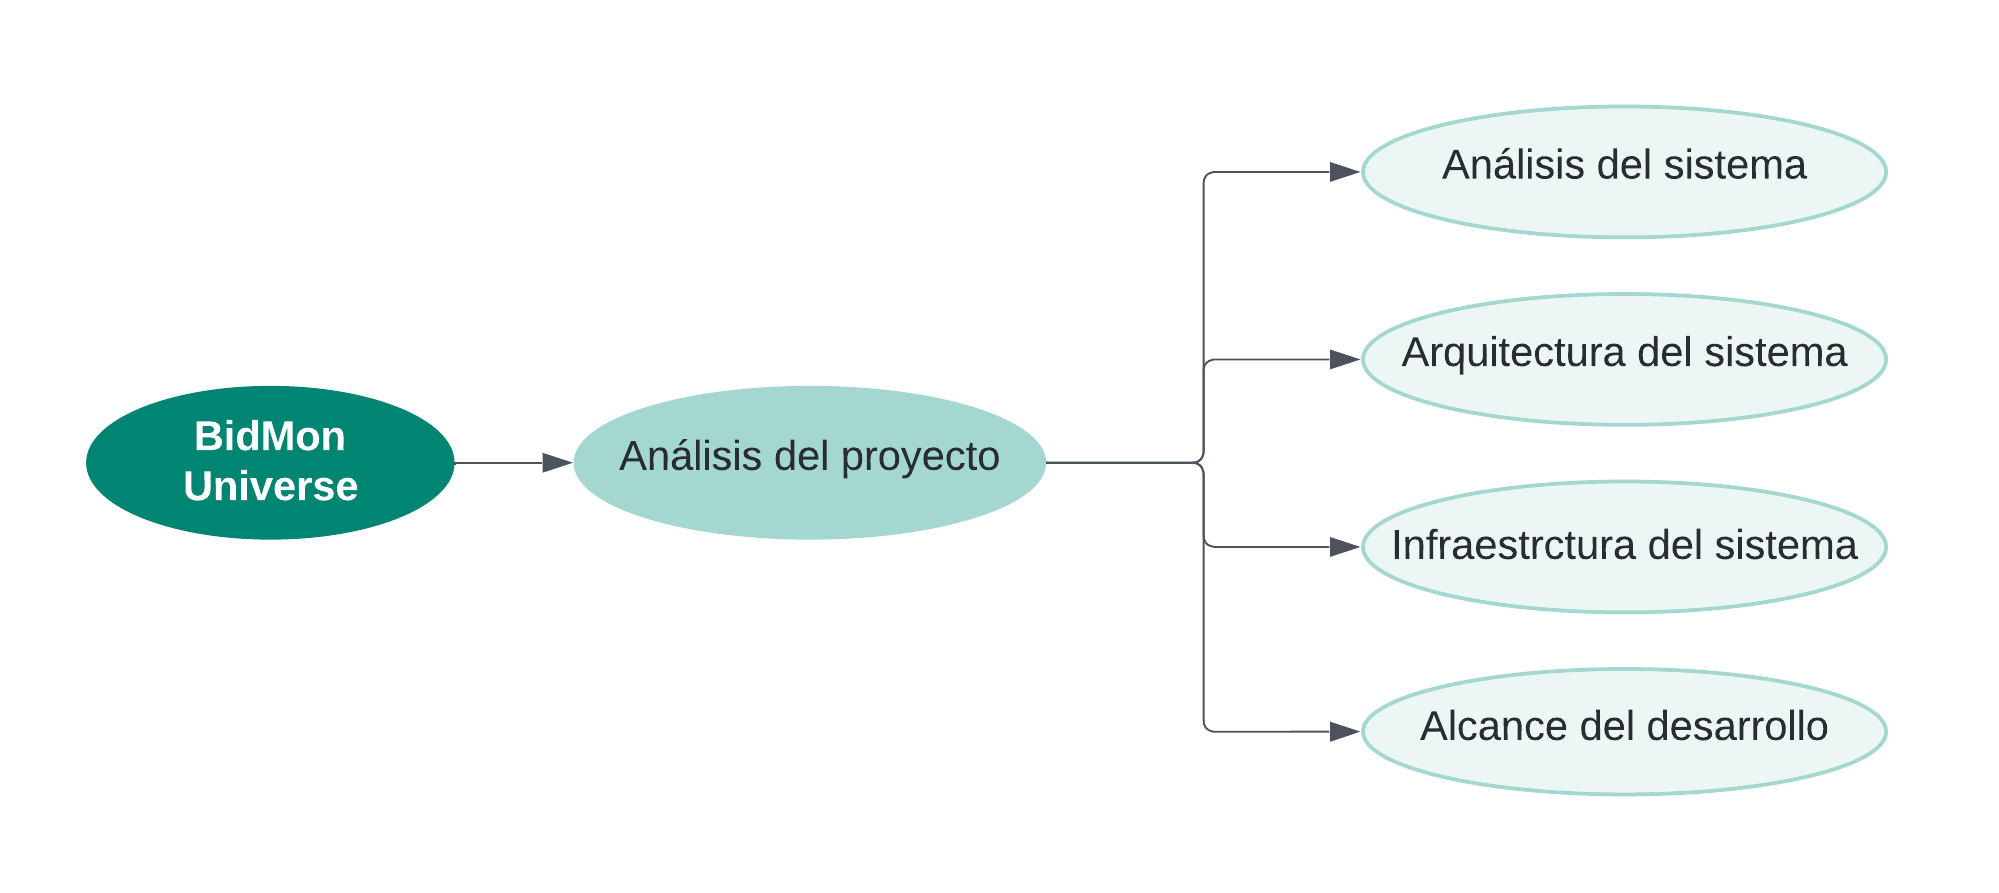
\includegraphics[width=0.7\linewidth]{figures/5-PBS/5_PBS-Analisis.png}
    \caption{PBS. Análisis del sistema}
    \label{fig:5_PBS-Analisis-Sistema}
\end{figure}

\subsubsection{PBS. Seguimiento del sistema}
En esta fase se detallan los productos que se obtienen en la fase de segumiento del proyecto, principalmente documentación e informes como se muestra en la \coloredUnderline{\hyperlink{fig:5_PBS-Seguimiento-Sistema}{Figura \ref*{fig:5_PBS-Seguimiento-Sistema}: \nameref*{fig:5_PBS-Seguimiento-Sistema}}}.
\begin{figure}[H]
    \hypertarget{fig:5_PBS-Seguimiento-Sistema}{}
    \centering
    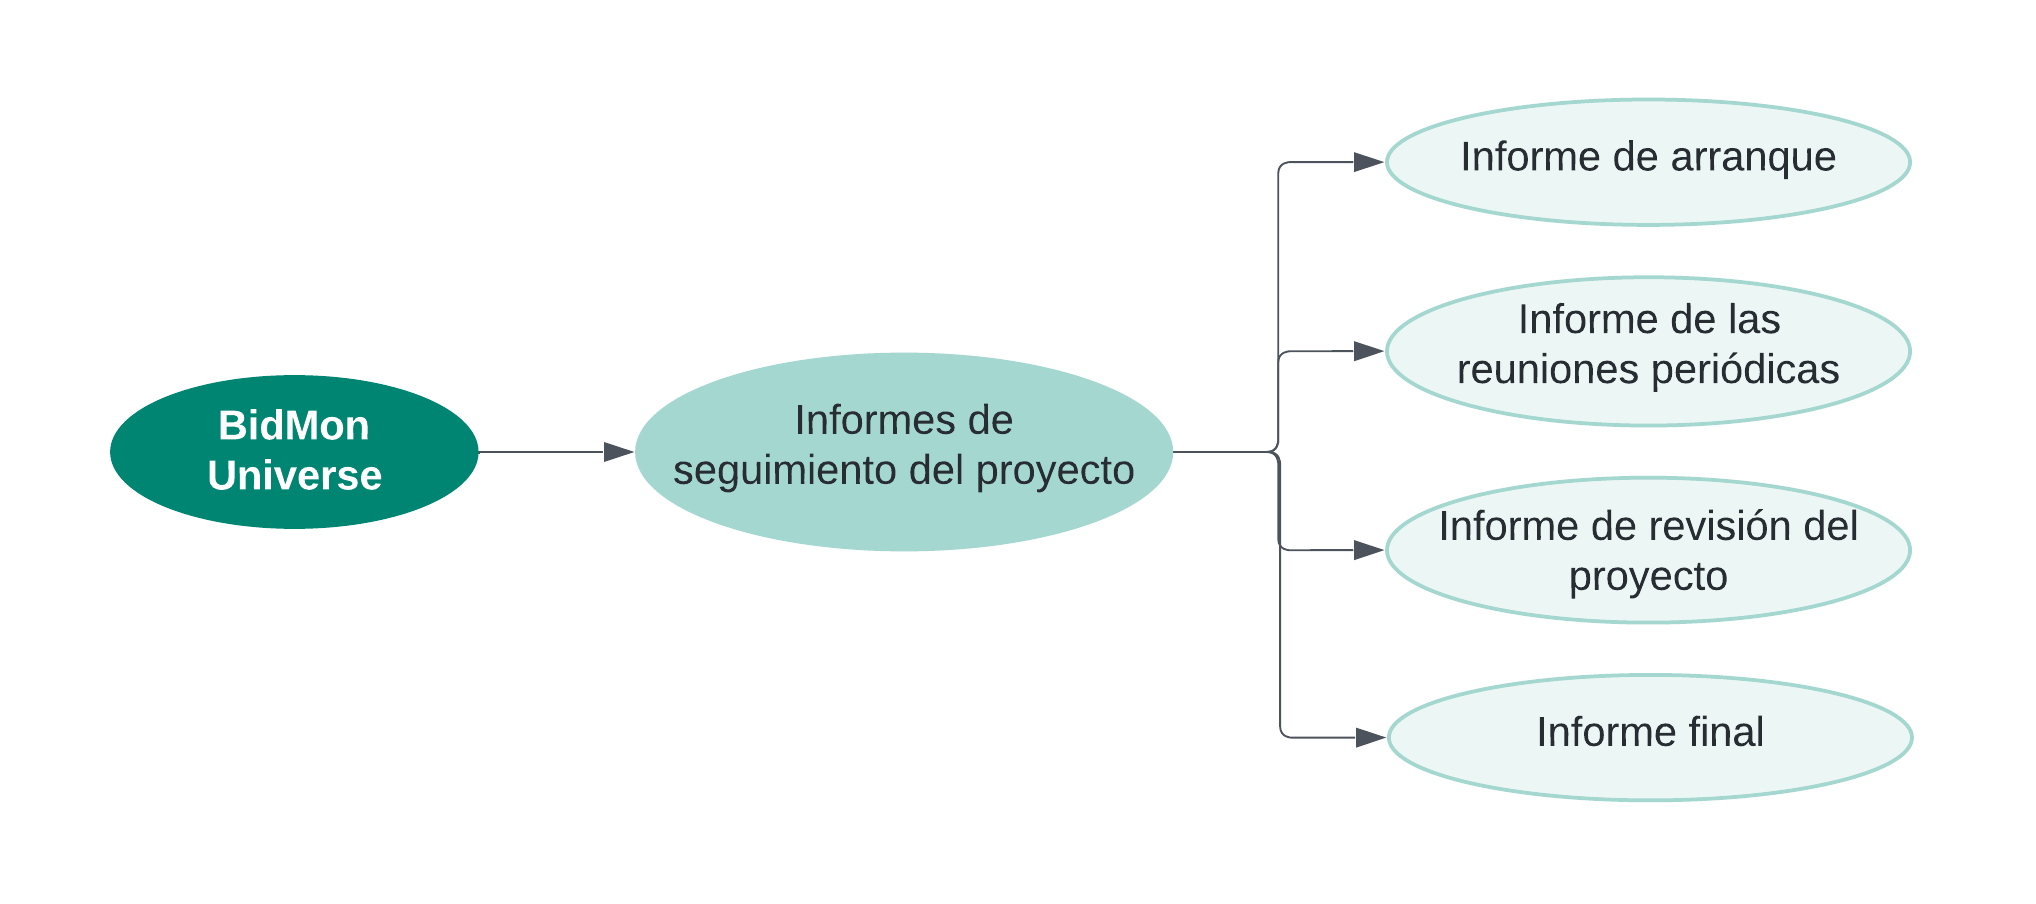
\includegraphics[width=0.7\linewidth]{figures/5-PBS/5_PBS-Seguimiento.png}
    \caption{PBS. Seguimiento del sistema}
    \label{fig:5_PBS-Seguimiento-Sistema}
\end{figure}

\subsubsection{PBS. Diseño del sistema}
En la \coloredUnderline{\hyperlink{fig:5_PBS-Diseño-Sistema}{Figura \ref*{fig:5_PBS-Diseño-Sistema}: \nameref*{fig:5_PBS-Diseño-Sistema}}}, se detallan los productos que se deben entregar en la fase de diseño del sistema.
\begin{figure}[H]
    \hypertarget{fig:5_PBS-Diseño-Sistema}{}
    \centering
    \includegraphics[width=0.9\linewidth]{figures/5-PBS/5_PBS-Diseno.png}
    \caption{PBS. Diseño del sistema}
    \label{fig:5_PBS-Diseño-Sistema}
\end{figure}

\subsubsection{PBS. Implementación del sistema}
En la \coloredUnderline{\hyperlink{fig:5_PBS-Implementación-Sistema}{Figura \ref*{fig:5_PBS-Implementación-Sistema}: \nameref*{fig:5_PBS-Implementación-Sistema}}}, se detallan los productos a realizar en la fase de implementación del sistema.
\begin{figure}[H]
    \hypertarget{fig:5_PBS-Implementación-Sistema}{}
    \centering
    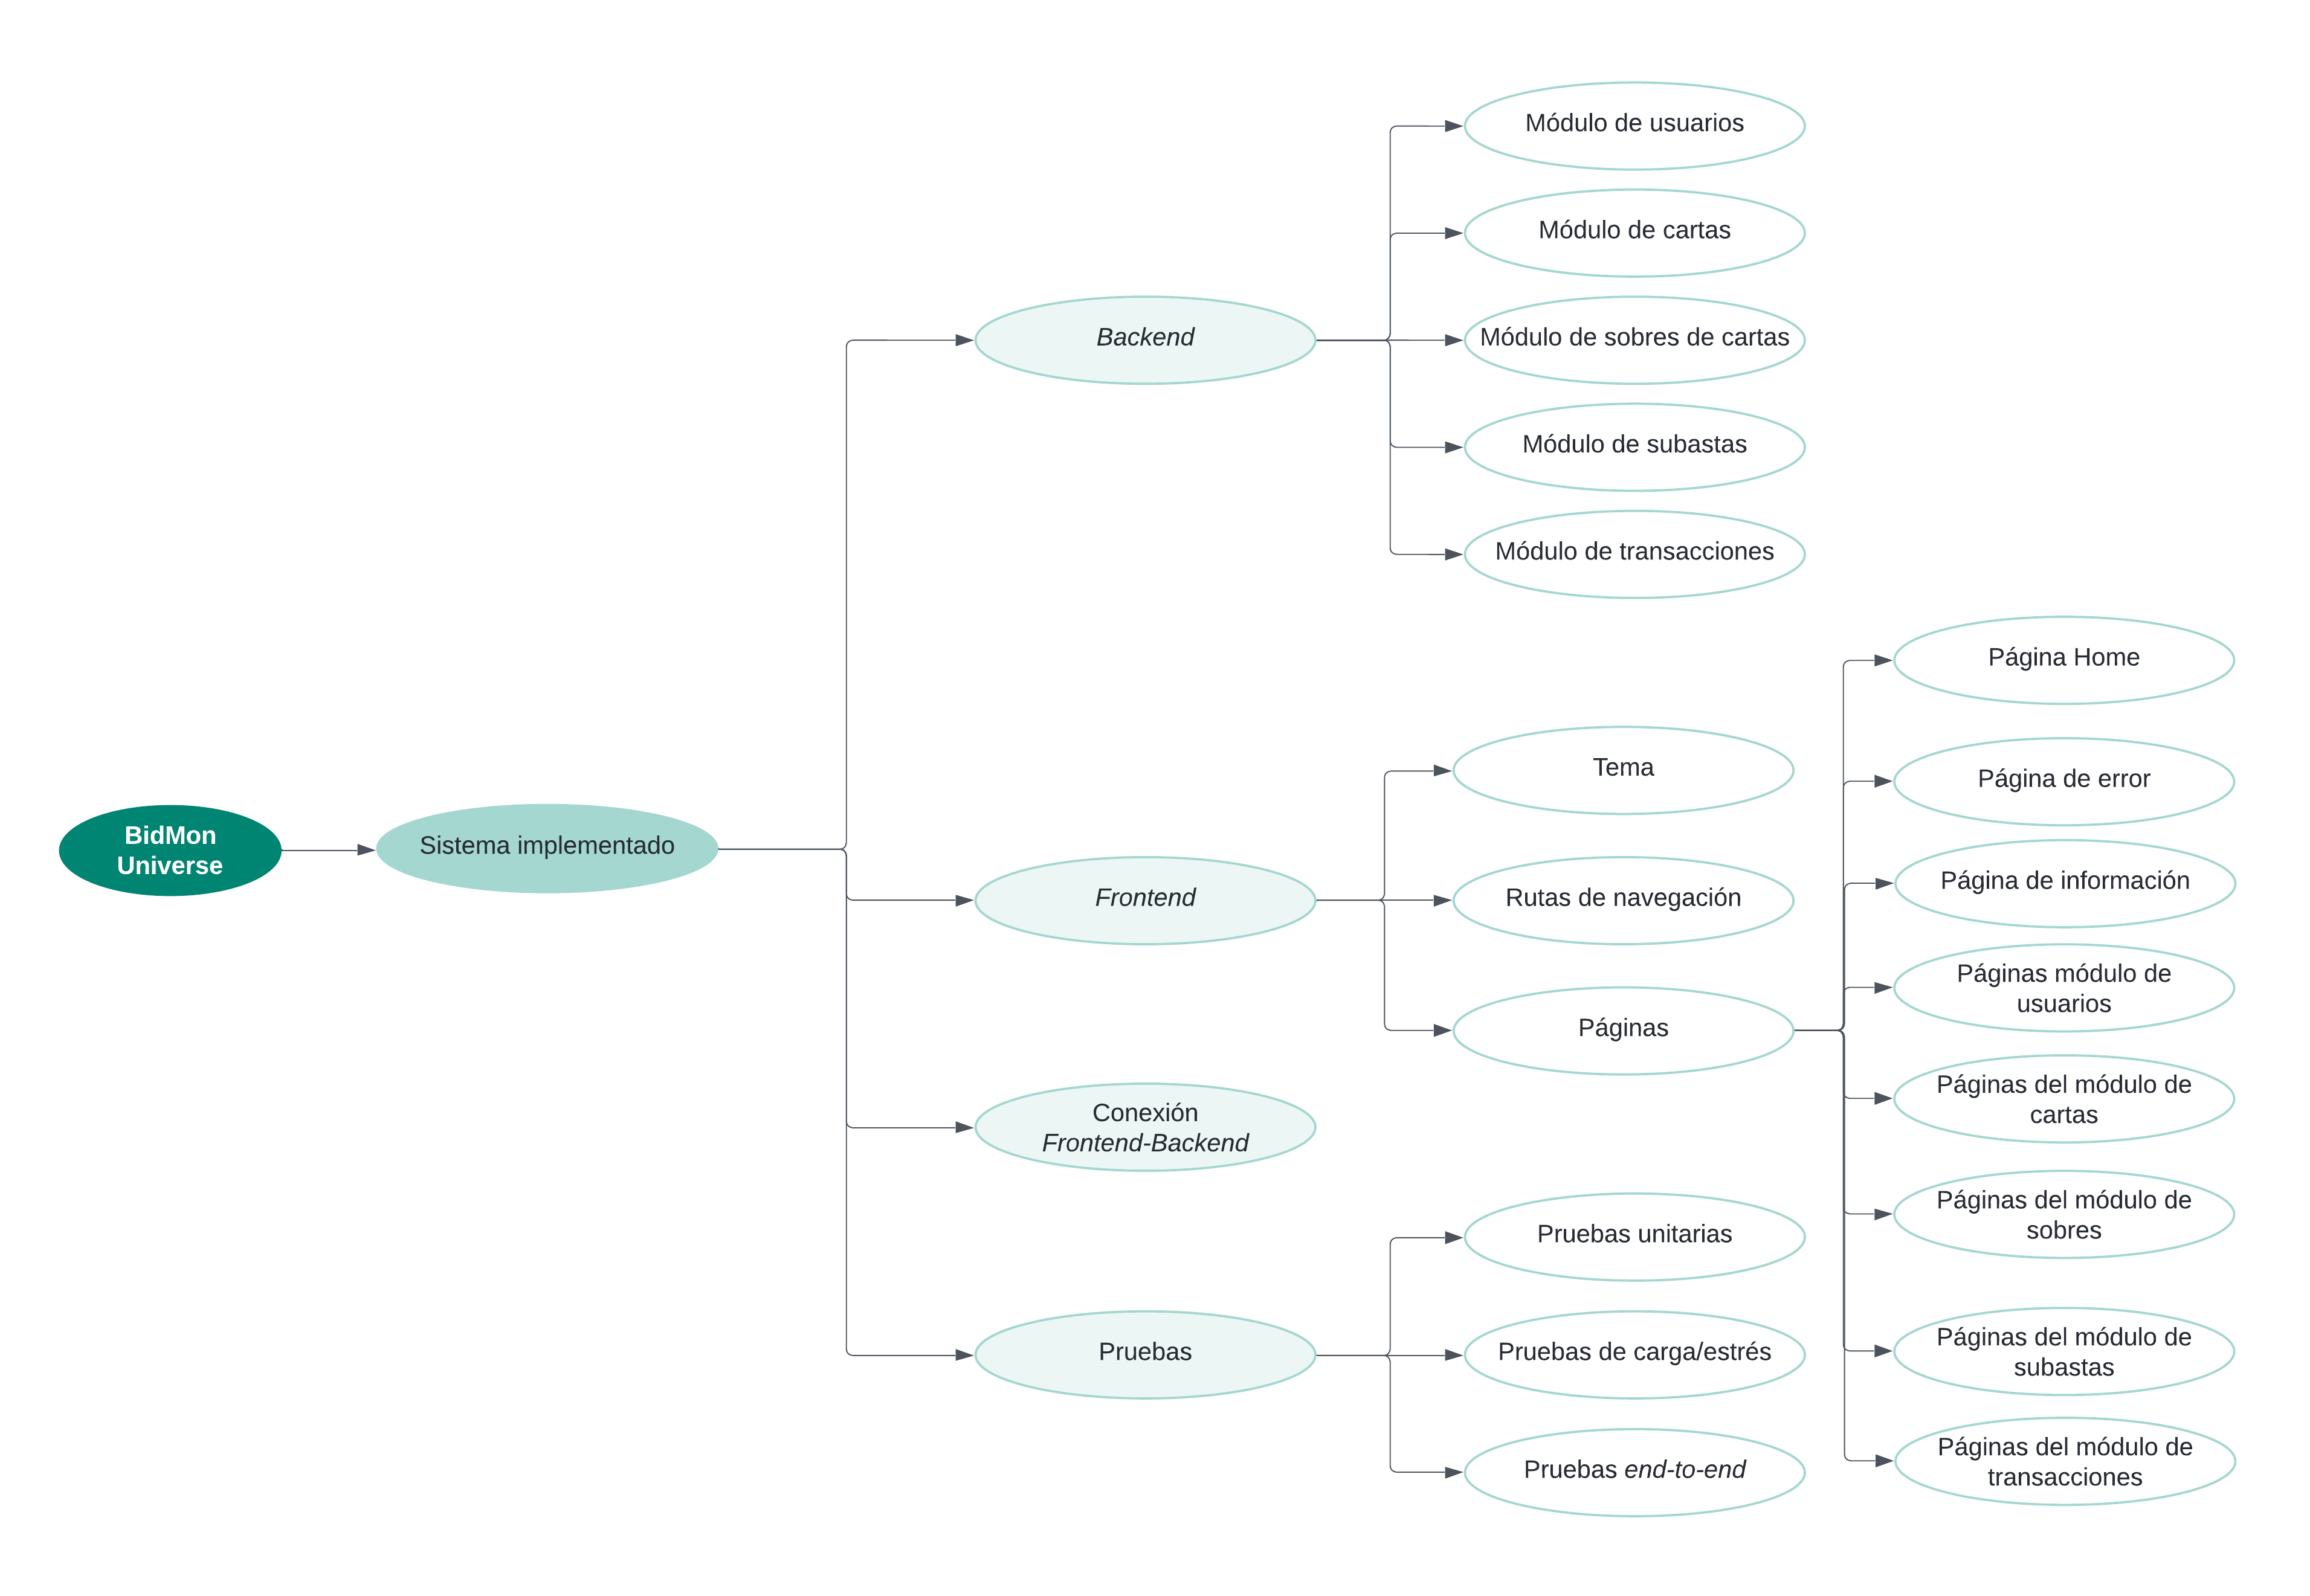
\includegraphics[width=0.9\linewidth]{figures/5-PBS/5_PBS-Implementacion.png}
    \caption{PBS. Implementación del sistema}
    \label{fig:5_PBS-Implementación-Sistema}
\end{figure}

\subsubsection{PBS. Pruebas del sistema}
En la fase de pruebas del sistema se obtienen como productos los resultados de la ejecución de dichas pruebas.
\begin{figure}[H]
    \hypertarget{fig:5_PBS-Pruebas-Sistema}{}
    \centering
    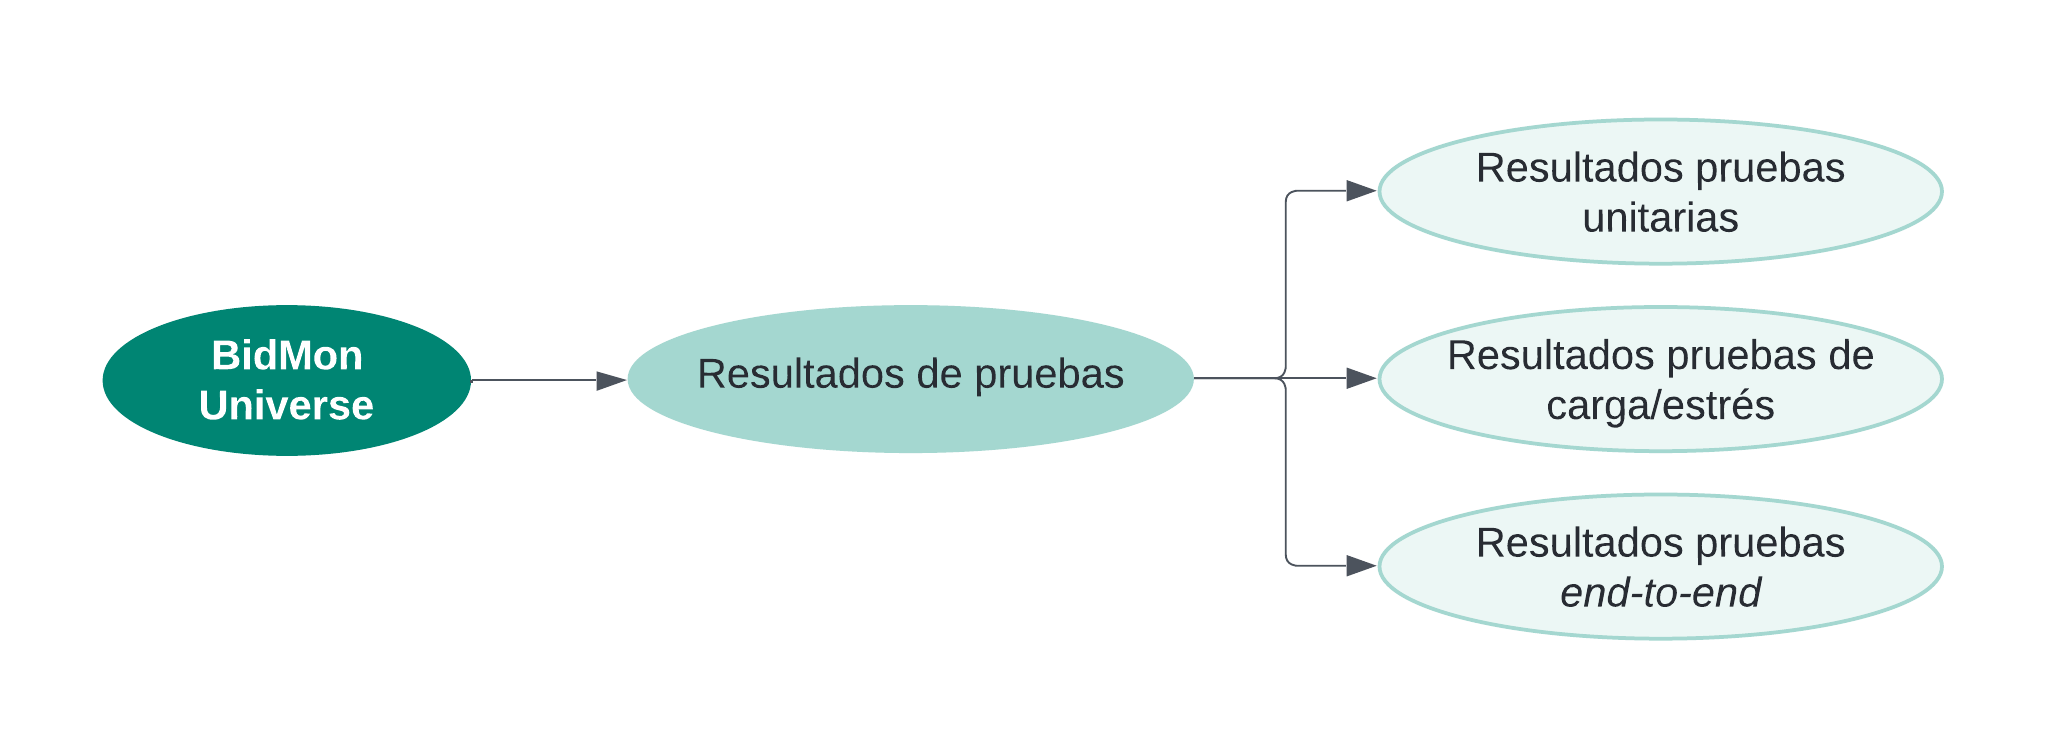
\includegraphics[width=0.7\linewidth]{figures/5-PBS/5_PBS-Pruebas.png}
    \caption{PBS. Pruebas del sistema}
    \label{fig:5_PBS-Pruebas-Sistema}
\end{figure}

\subsubsection{PBS. Despliegue del sistema}
En la fase de despliegue del sistema se obtiene como producto el sistema desplegado y en funcionamiento.
\begin{figure}[H]
    \hypertarget{fig:5_PBS-Despliegue-Sistema}{}
    \centering
    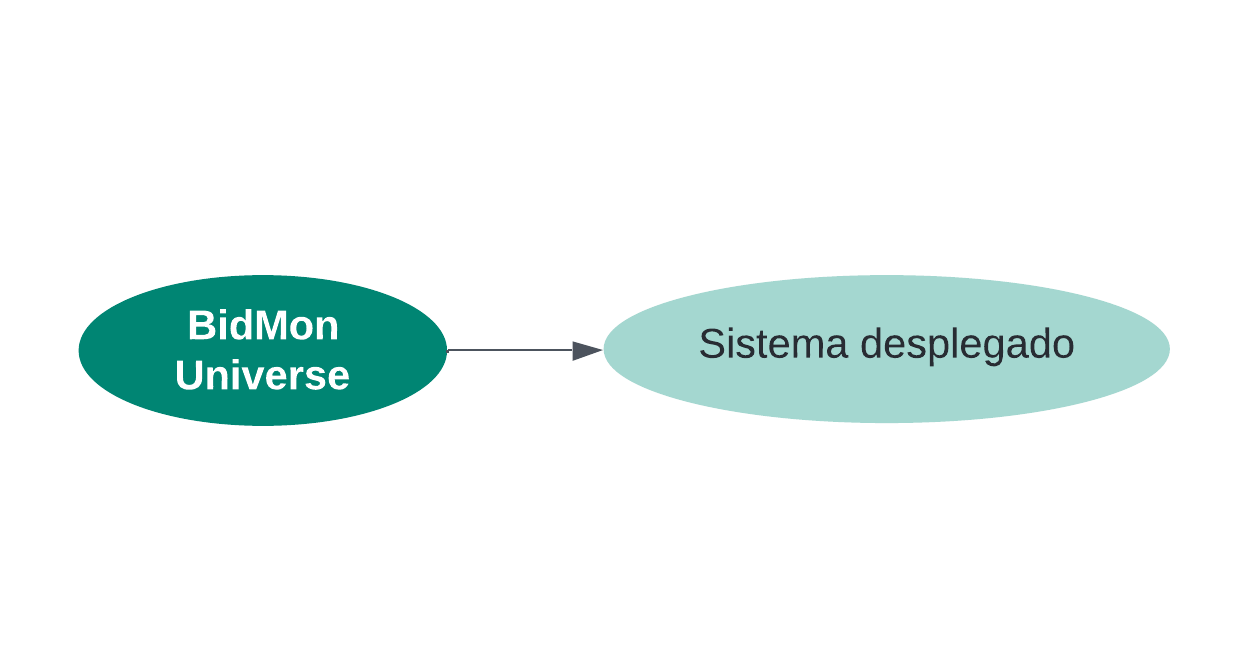
\includegraphics[width=0.7\linewidth]{figures/5-PBS/5_PBS-Despliegue.png}
    \caption{PBS. Despliegue del sistema}
    \label{fig:5_PBS-Despliegue-Sistema}
\end{figure}


\subsubsection{PBS. Documentación del sistema}
En la fase de documentación del sistema se obtienen como productos los documentos técnicos que describen el proyecto junto con los anexos.
\begin{figure}[H]
    \hypertarget{fig:5_PBS-Documentación-Sistema}{}
    \centering
    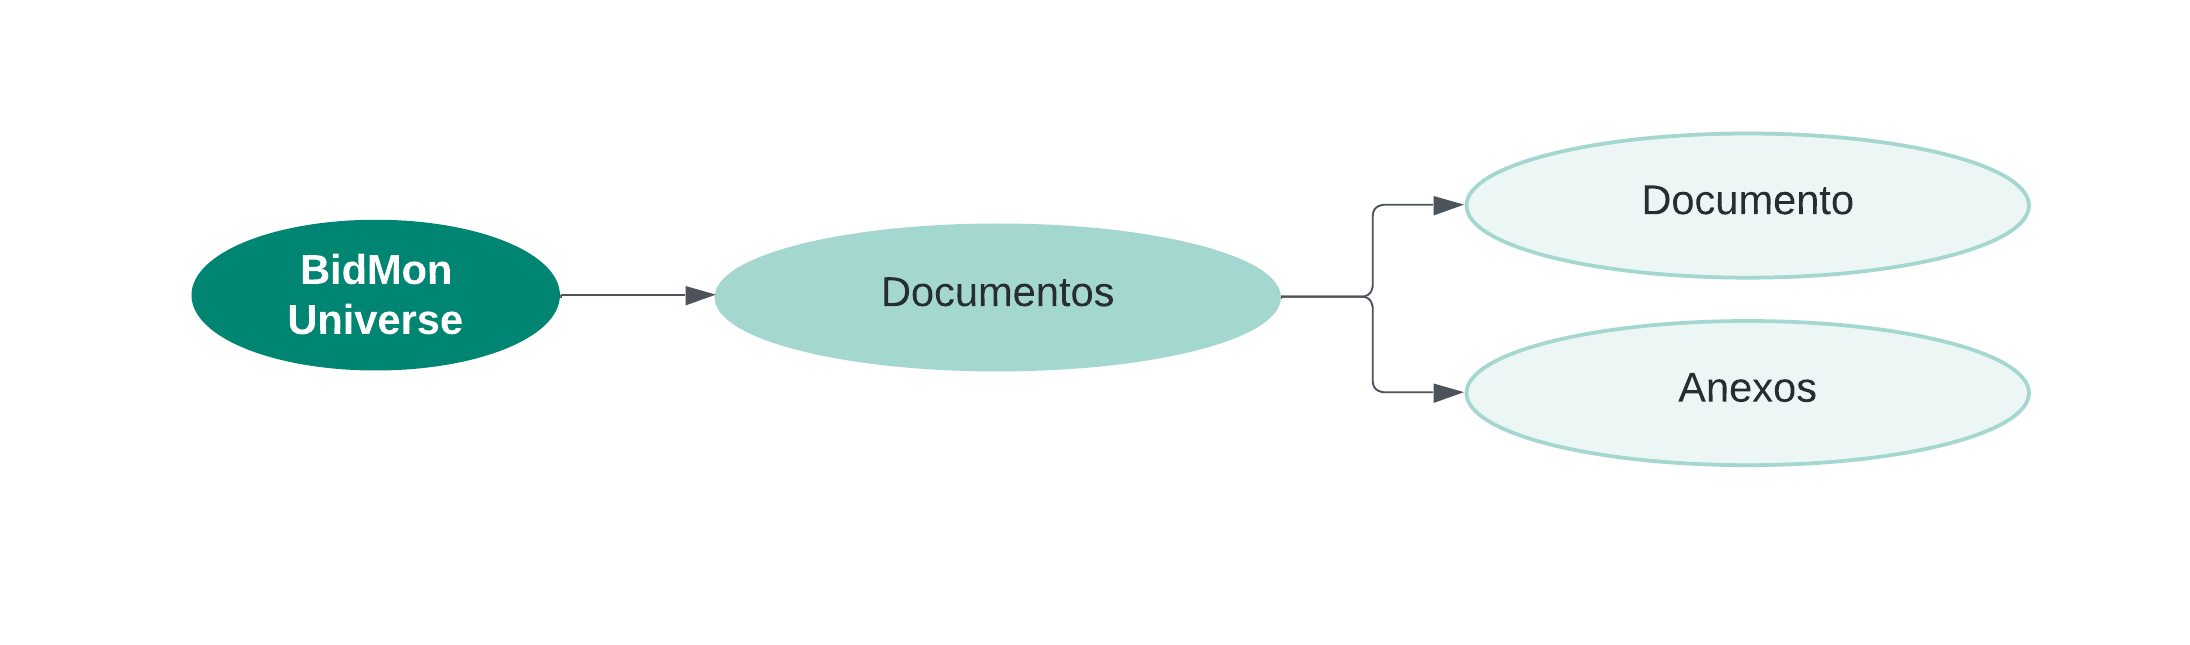
\includegraphics[width=0.7\linewidth]{figures/5-PBS/5_PBS-Documento.png}
    \caption{PBS. Documentación del sistema}
    \label{fig:5_PBS-Documentación-Sistema}
\end{figure}



\subsection{Planificación Inicial. WBS}
\subsubsection{WBS}
En esta sección se detalla la estructura de desglose del trabajo del proyecto también conocida como WBS, \textit{Work Breakdown Structure}. 
En ella se especifican las tareas necesarias para obtener los productos detallados en \coloredUnderline{\hyperlink{sec:5-PBS}{\ref*{sec:5-PBS} \nameref*{sec:5-PBS}}}.

Estas tareas se representan en forma de árbol jerárquico, donde cada rama representa una tarea y sus subramas las tareas que la componen.
El diagrama se ha dividido en las fases en las que se divide el proyecto para mejorar la legibilidad, facilitando la comprensión de las tareas y sub-tareas que se deben realizar en cada una de ellas.

\subsubsubsection{WBS. Visión general}
En la \coloredUnderline{\hyperlink{fig:5_WBS-Vision-General}{Figura \ref*{fig:5_WBS-Vision-General}: \nameref*{fig:5_WBS-Vision-General}}} se muestra la estructura de desglose del trabajo del proyecto de alto nivel, es decir, 
las tareas generales o fases que se deben realizar para cumplir con los objetivos del proyecto.
En las siguientes secciones, se entrará en detalle en cada una de las tareas.
\begin{figure}[H]
    \hypertarget{fig:5_WBS-Vision-General}{}
    \centering
    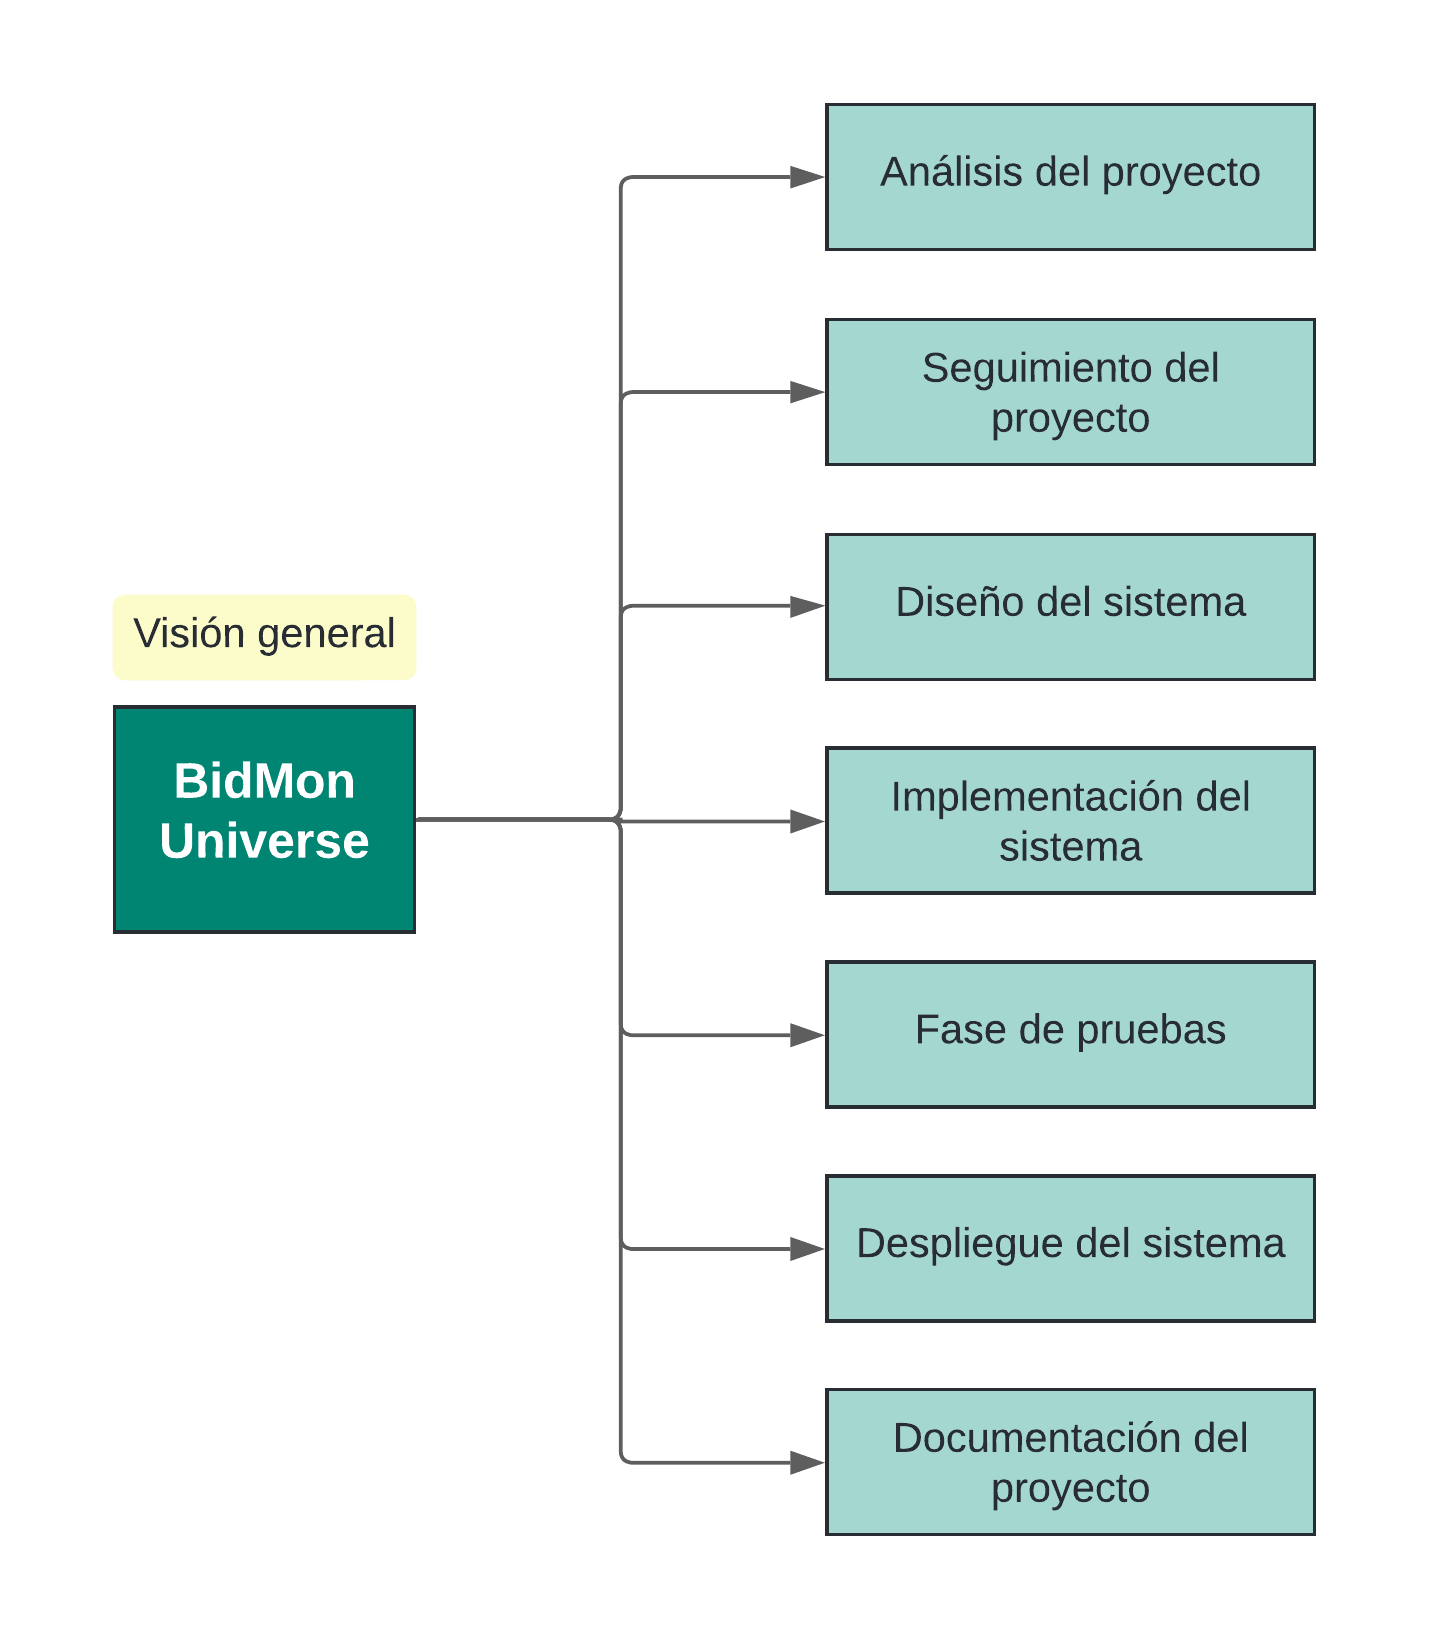
\includegraphics[width=0.5\linewidth]{figures/5-WBS/5_WBS-Vision-General.png}
    \caption{WBS. Visión general}
    \label{fig:5_WBS-Vision-General}
\end{figure}

\subsubsubsection{WBS. Análisis del proyecto}
En la \coloredUnderline{\hyperlink{fig:5_WBS-Analisis}{Figura \ref*{fig:5_WBS-Analisis}: \nameref*{fig:5_WBS-Analisis}}}, se detallan las tareas que se deben realizar en la fase de análisis del sistema para cumplir con los objetivos del proyecto.
\begin{figure}[H]
    \hypertarget{fig:5_WBS-Analisis}{}
    \centering
    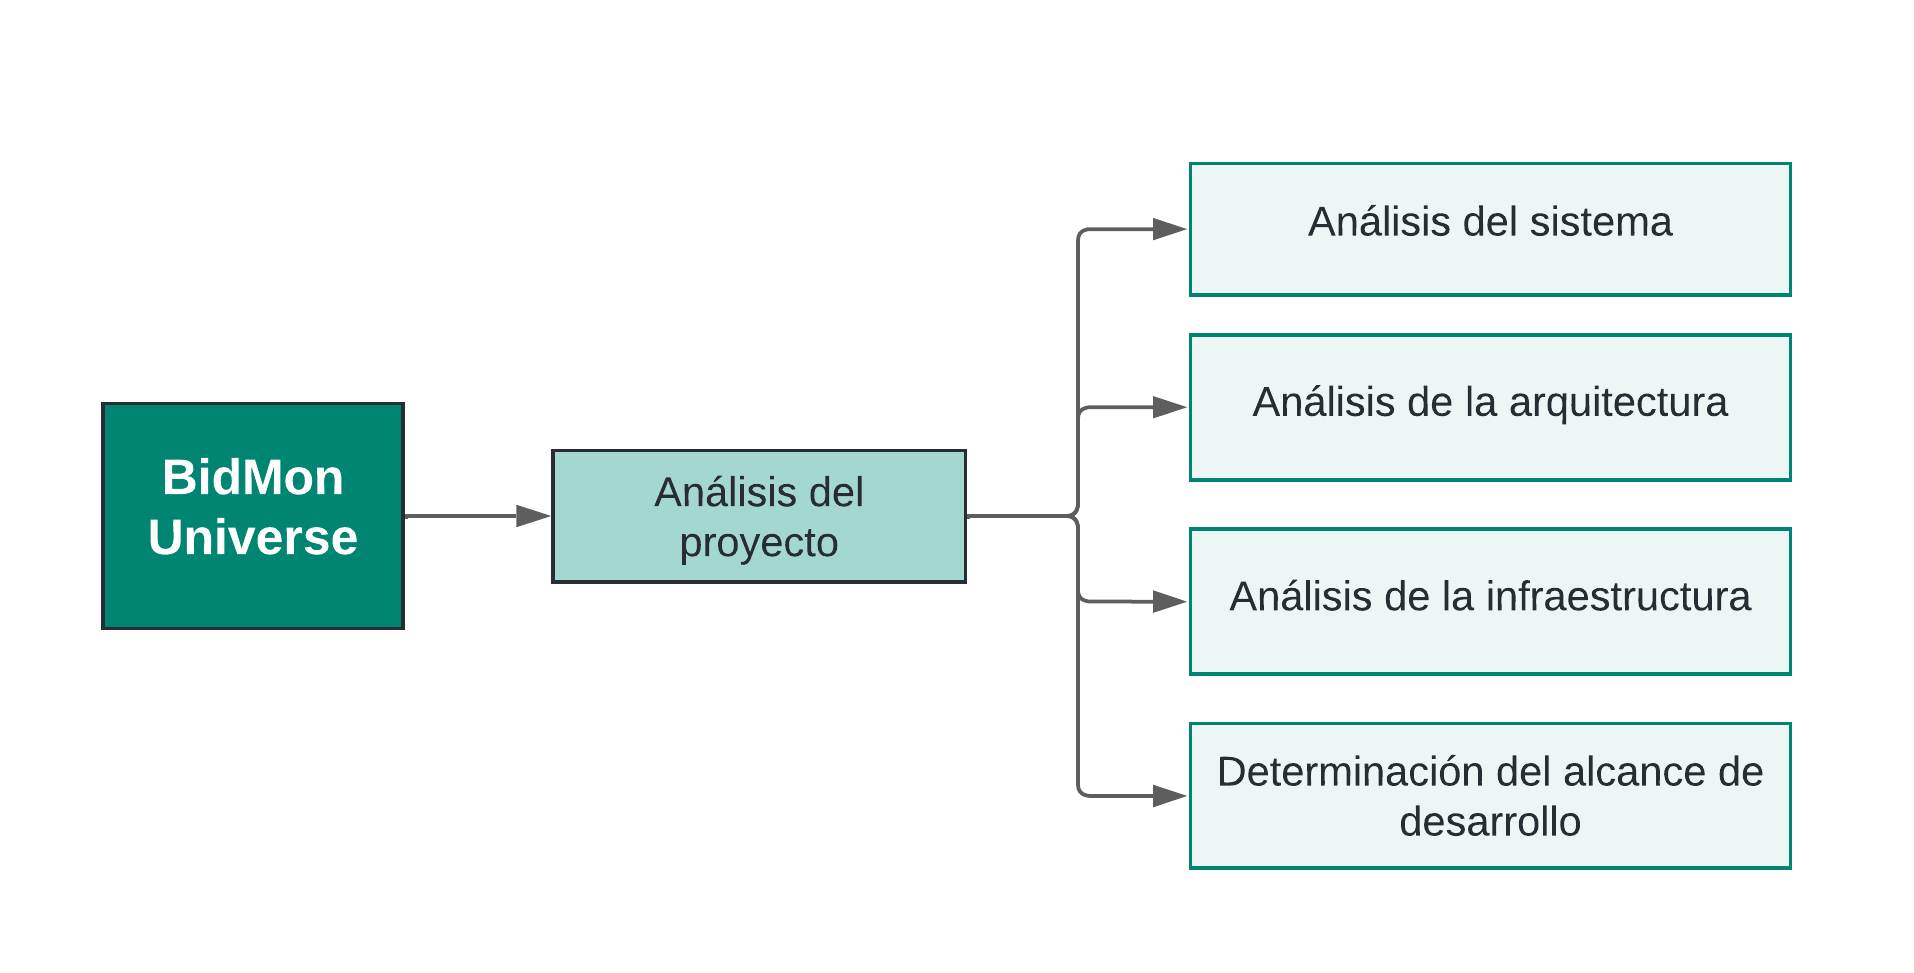
\includegraphics[width=0.7\linewidth]{figures/5-WBS/5_WBS-Analisis.png}
    \caption{WBS. Análisis del proyecto}
    \label{fig:5_WBS-Analisis}
\end{figure}

\subsubsubsection{WBS. Seguimiento del sistema}
En esta fase se realizan las tareas de seguimiento del proyecto, a través de distintas reuniones en las que se recopilará infomarción sobre el avance del proyecto. 
\begin{figure}[H]
    \hypertarget{fig:5_WBS-Seguimiento}{}
    \centering
    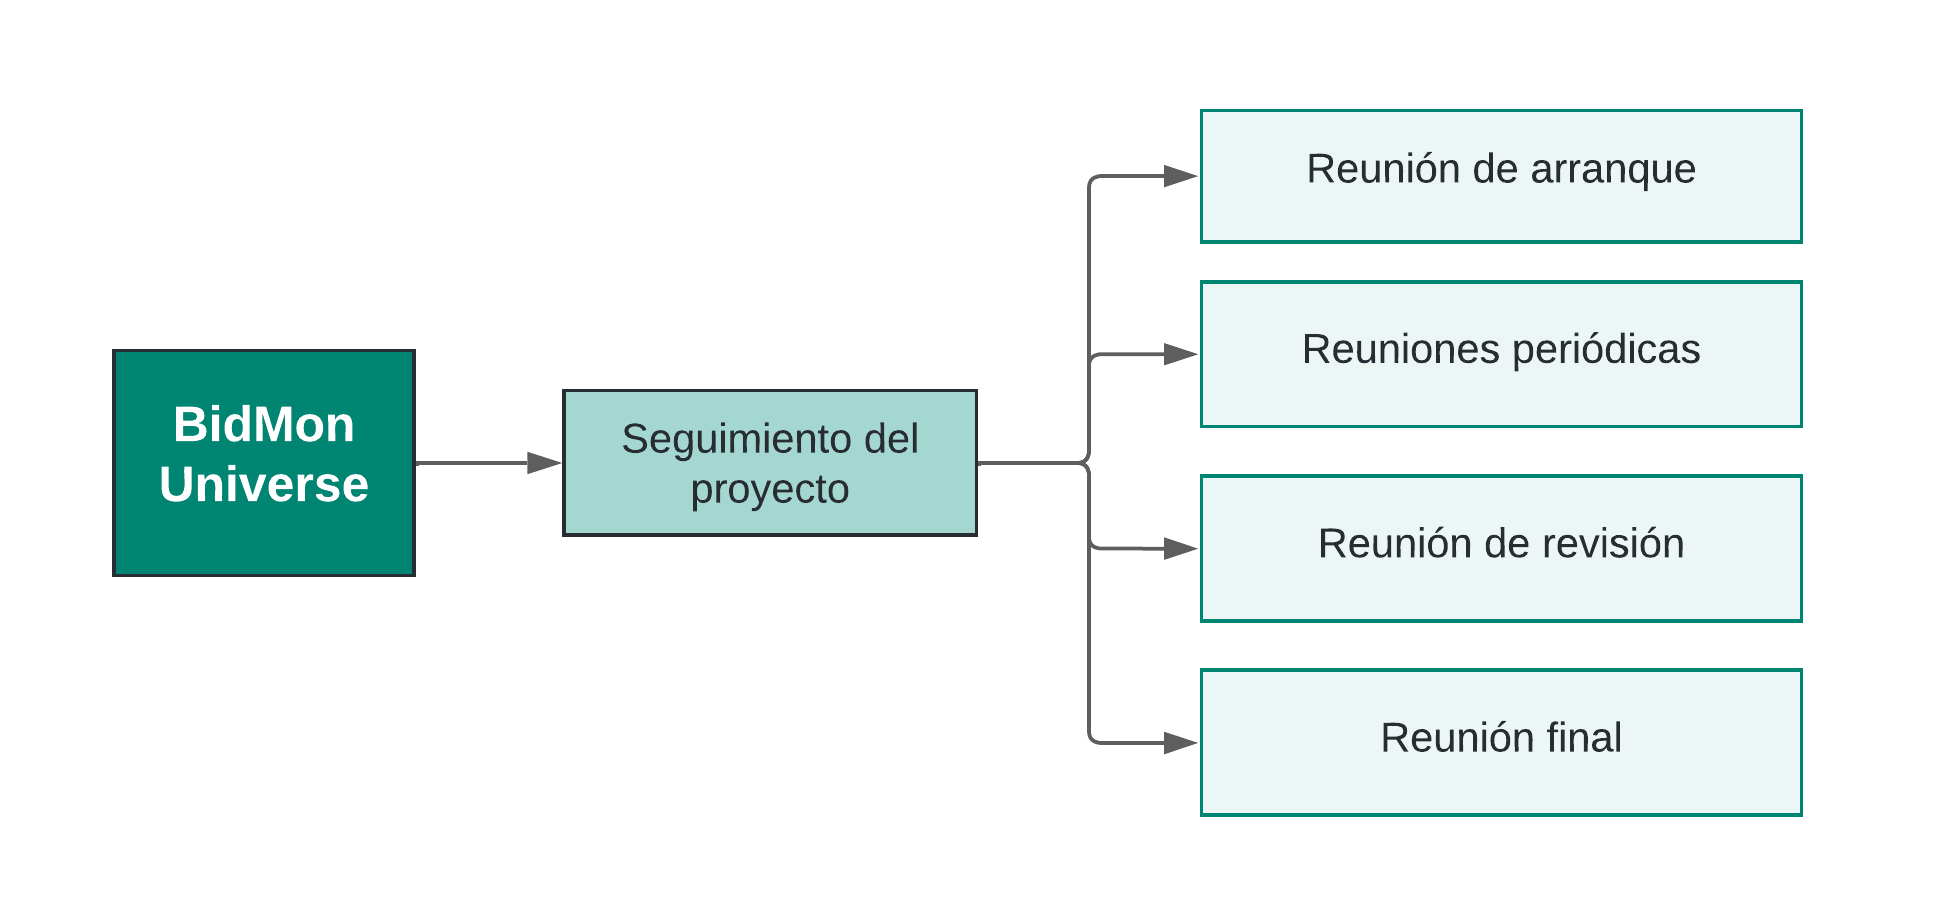
\includegraphics[width=0.7\linewidth]{figures/5-WBS/5_WBS-Seguimiento.png}
    \caption{WBS. Seguimiento del sistema}
    \label{fig:5_WBS-Seguimiento}
\end{figure}

\subsubsubsection{WBS. Diseño del sistema}
En la \coloredUnderline{\hyperlink{fig:5_WBS-Diseno}{Figura \ref*{fig:5_WBS-Diseno}: \nameref*{fig:5_WBS-Diseno}}}, se detallan las tareas que se deben realizar en la fase de diseño del sistema.
\begin{figure}[H]
    \hypertarget{fig:5_WBS-Diseno}{}
    \centering
    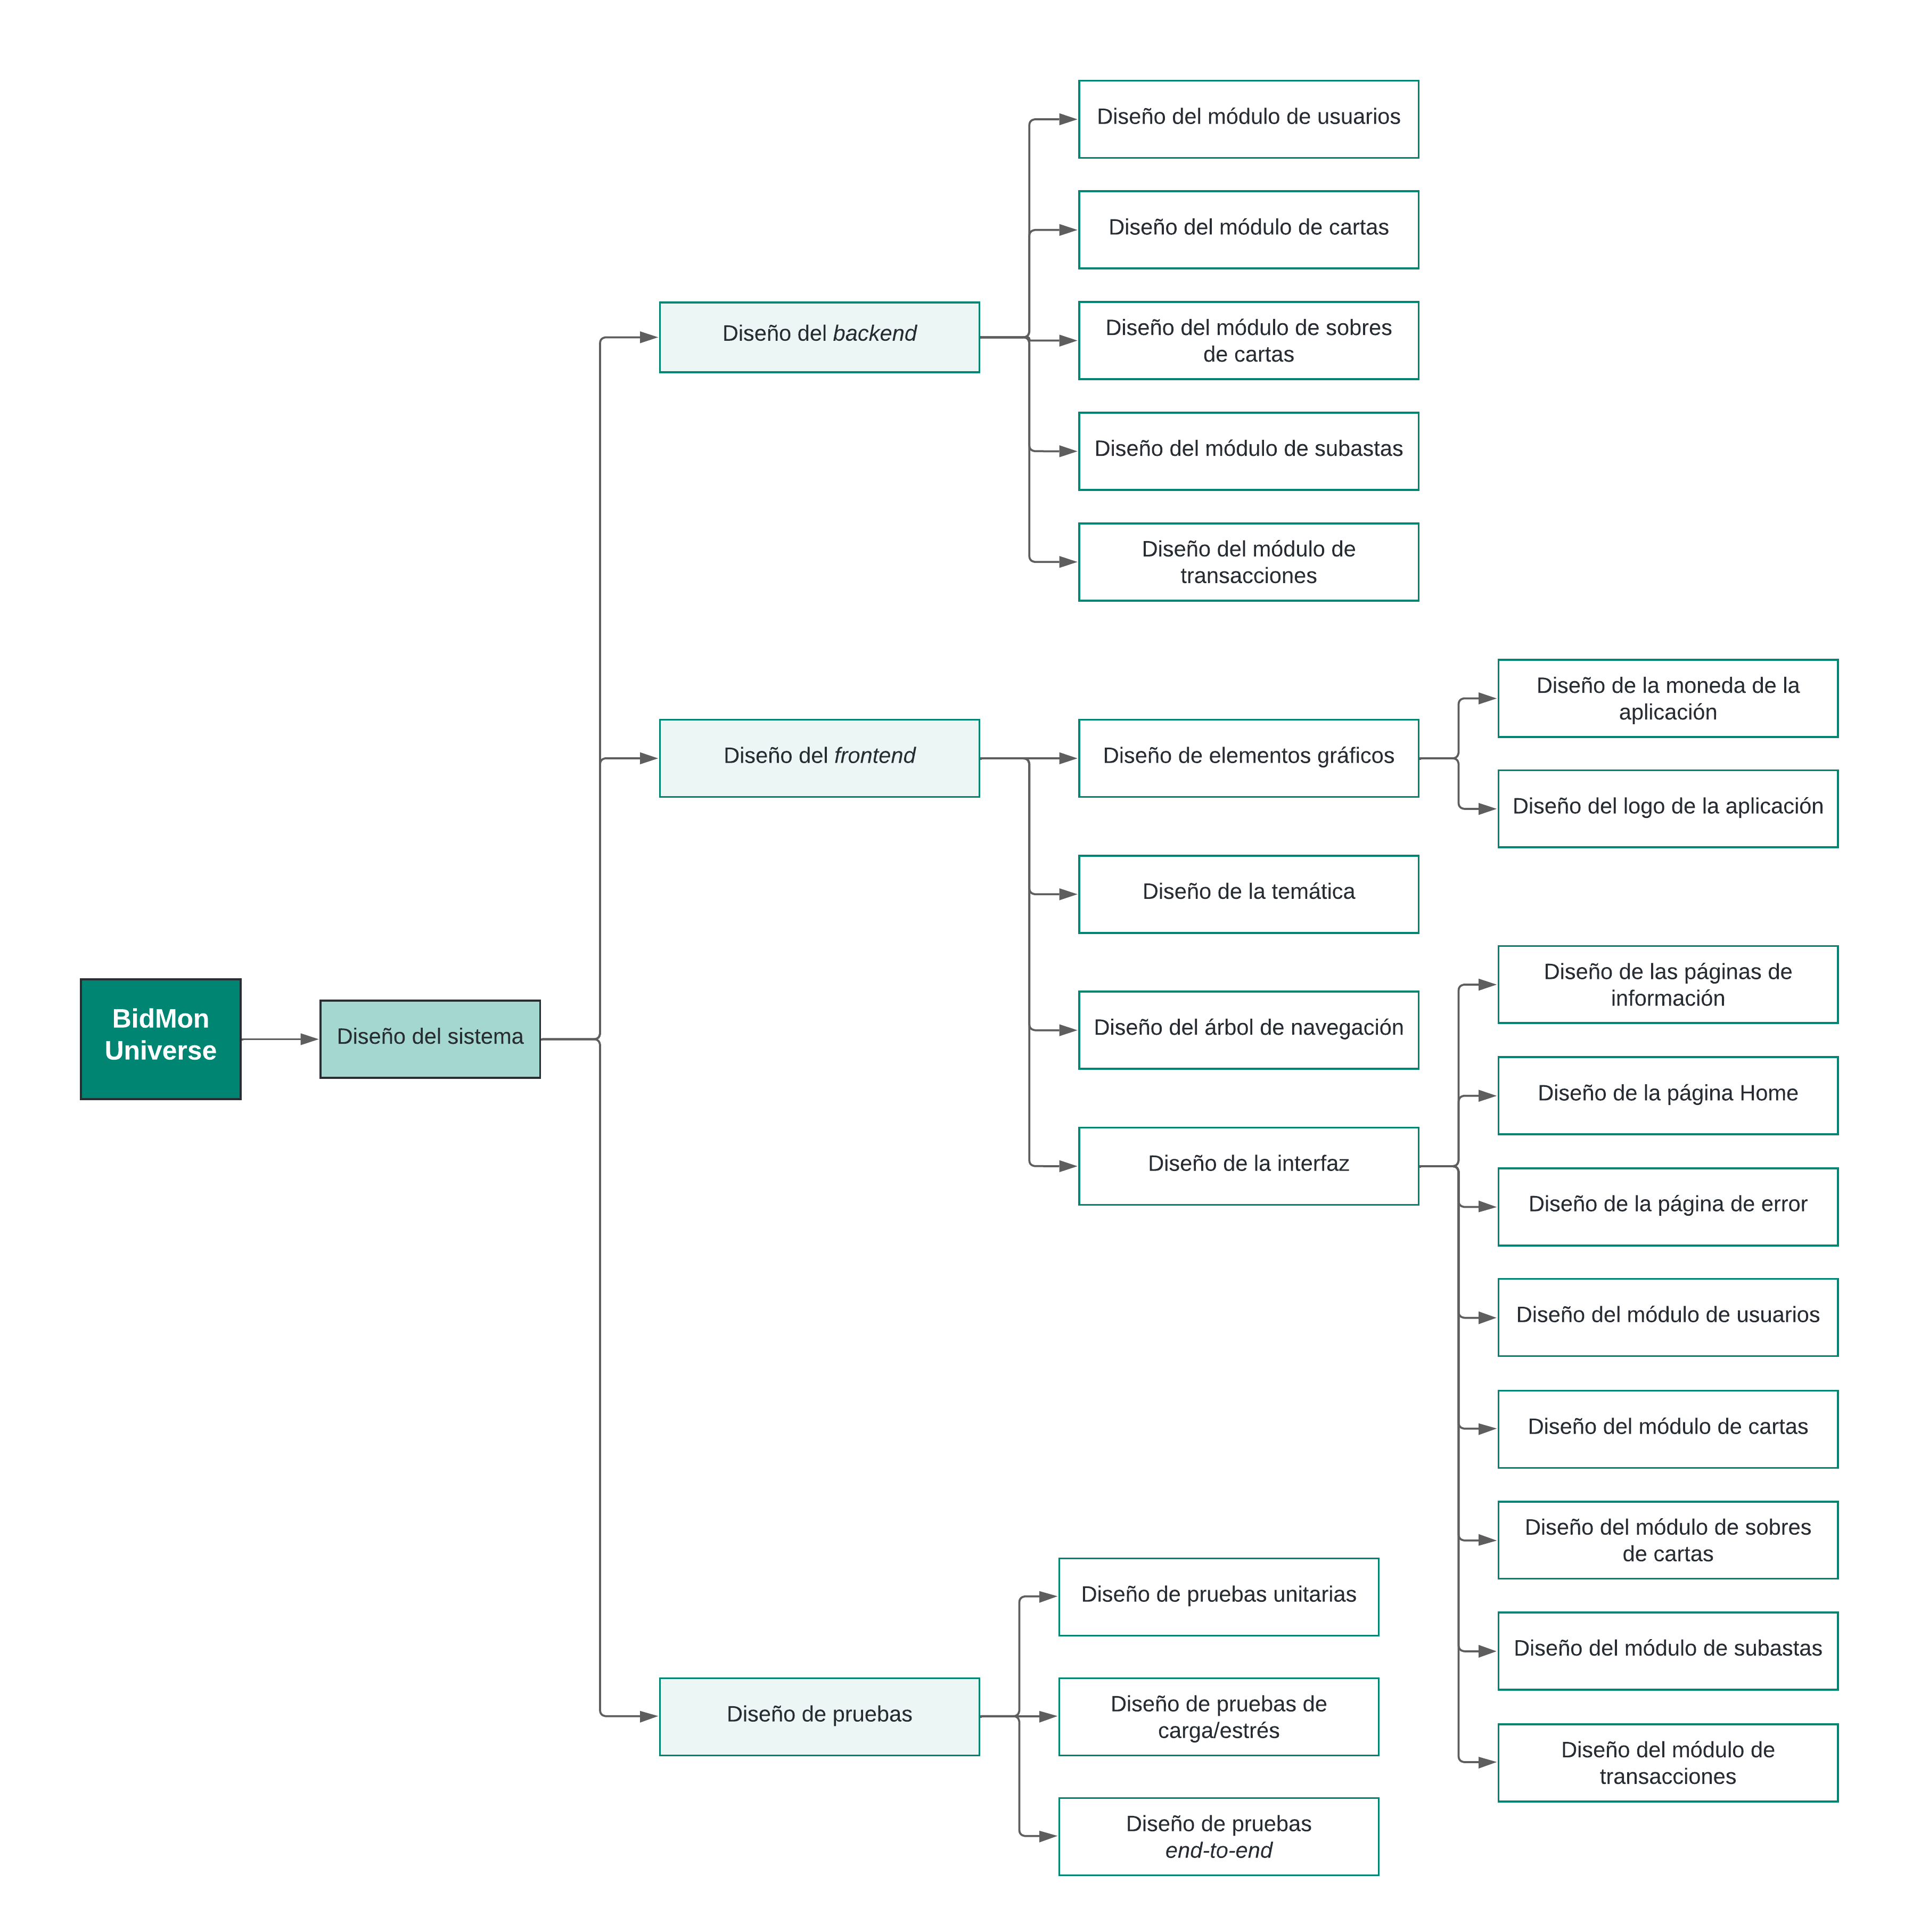
\includegraphics[width=0.9\linewidth]{figures/5-WBS/5_WBS-Diseno.png}
    \caption{WBS. Diseño del sistema}
    \label{fig:5_WBS-Diseno}
\end{figure}

\subsubsubsection{WBS. Implementación del sistema}
En la \coloredUnderline{\hyperlink{fig:5_WBS-Implementacion}{Figura \ref*{fig:5_WBS-Implementacion}: \nameref*{fig:5_WBS-Implementacion}}}, se detallan las tareas que se deben realizar en la fase de implementación del sistema.
\begin{figure}[H]
    \hypertarget{fig:5_WBS-Implementacion}{}
    \centering
    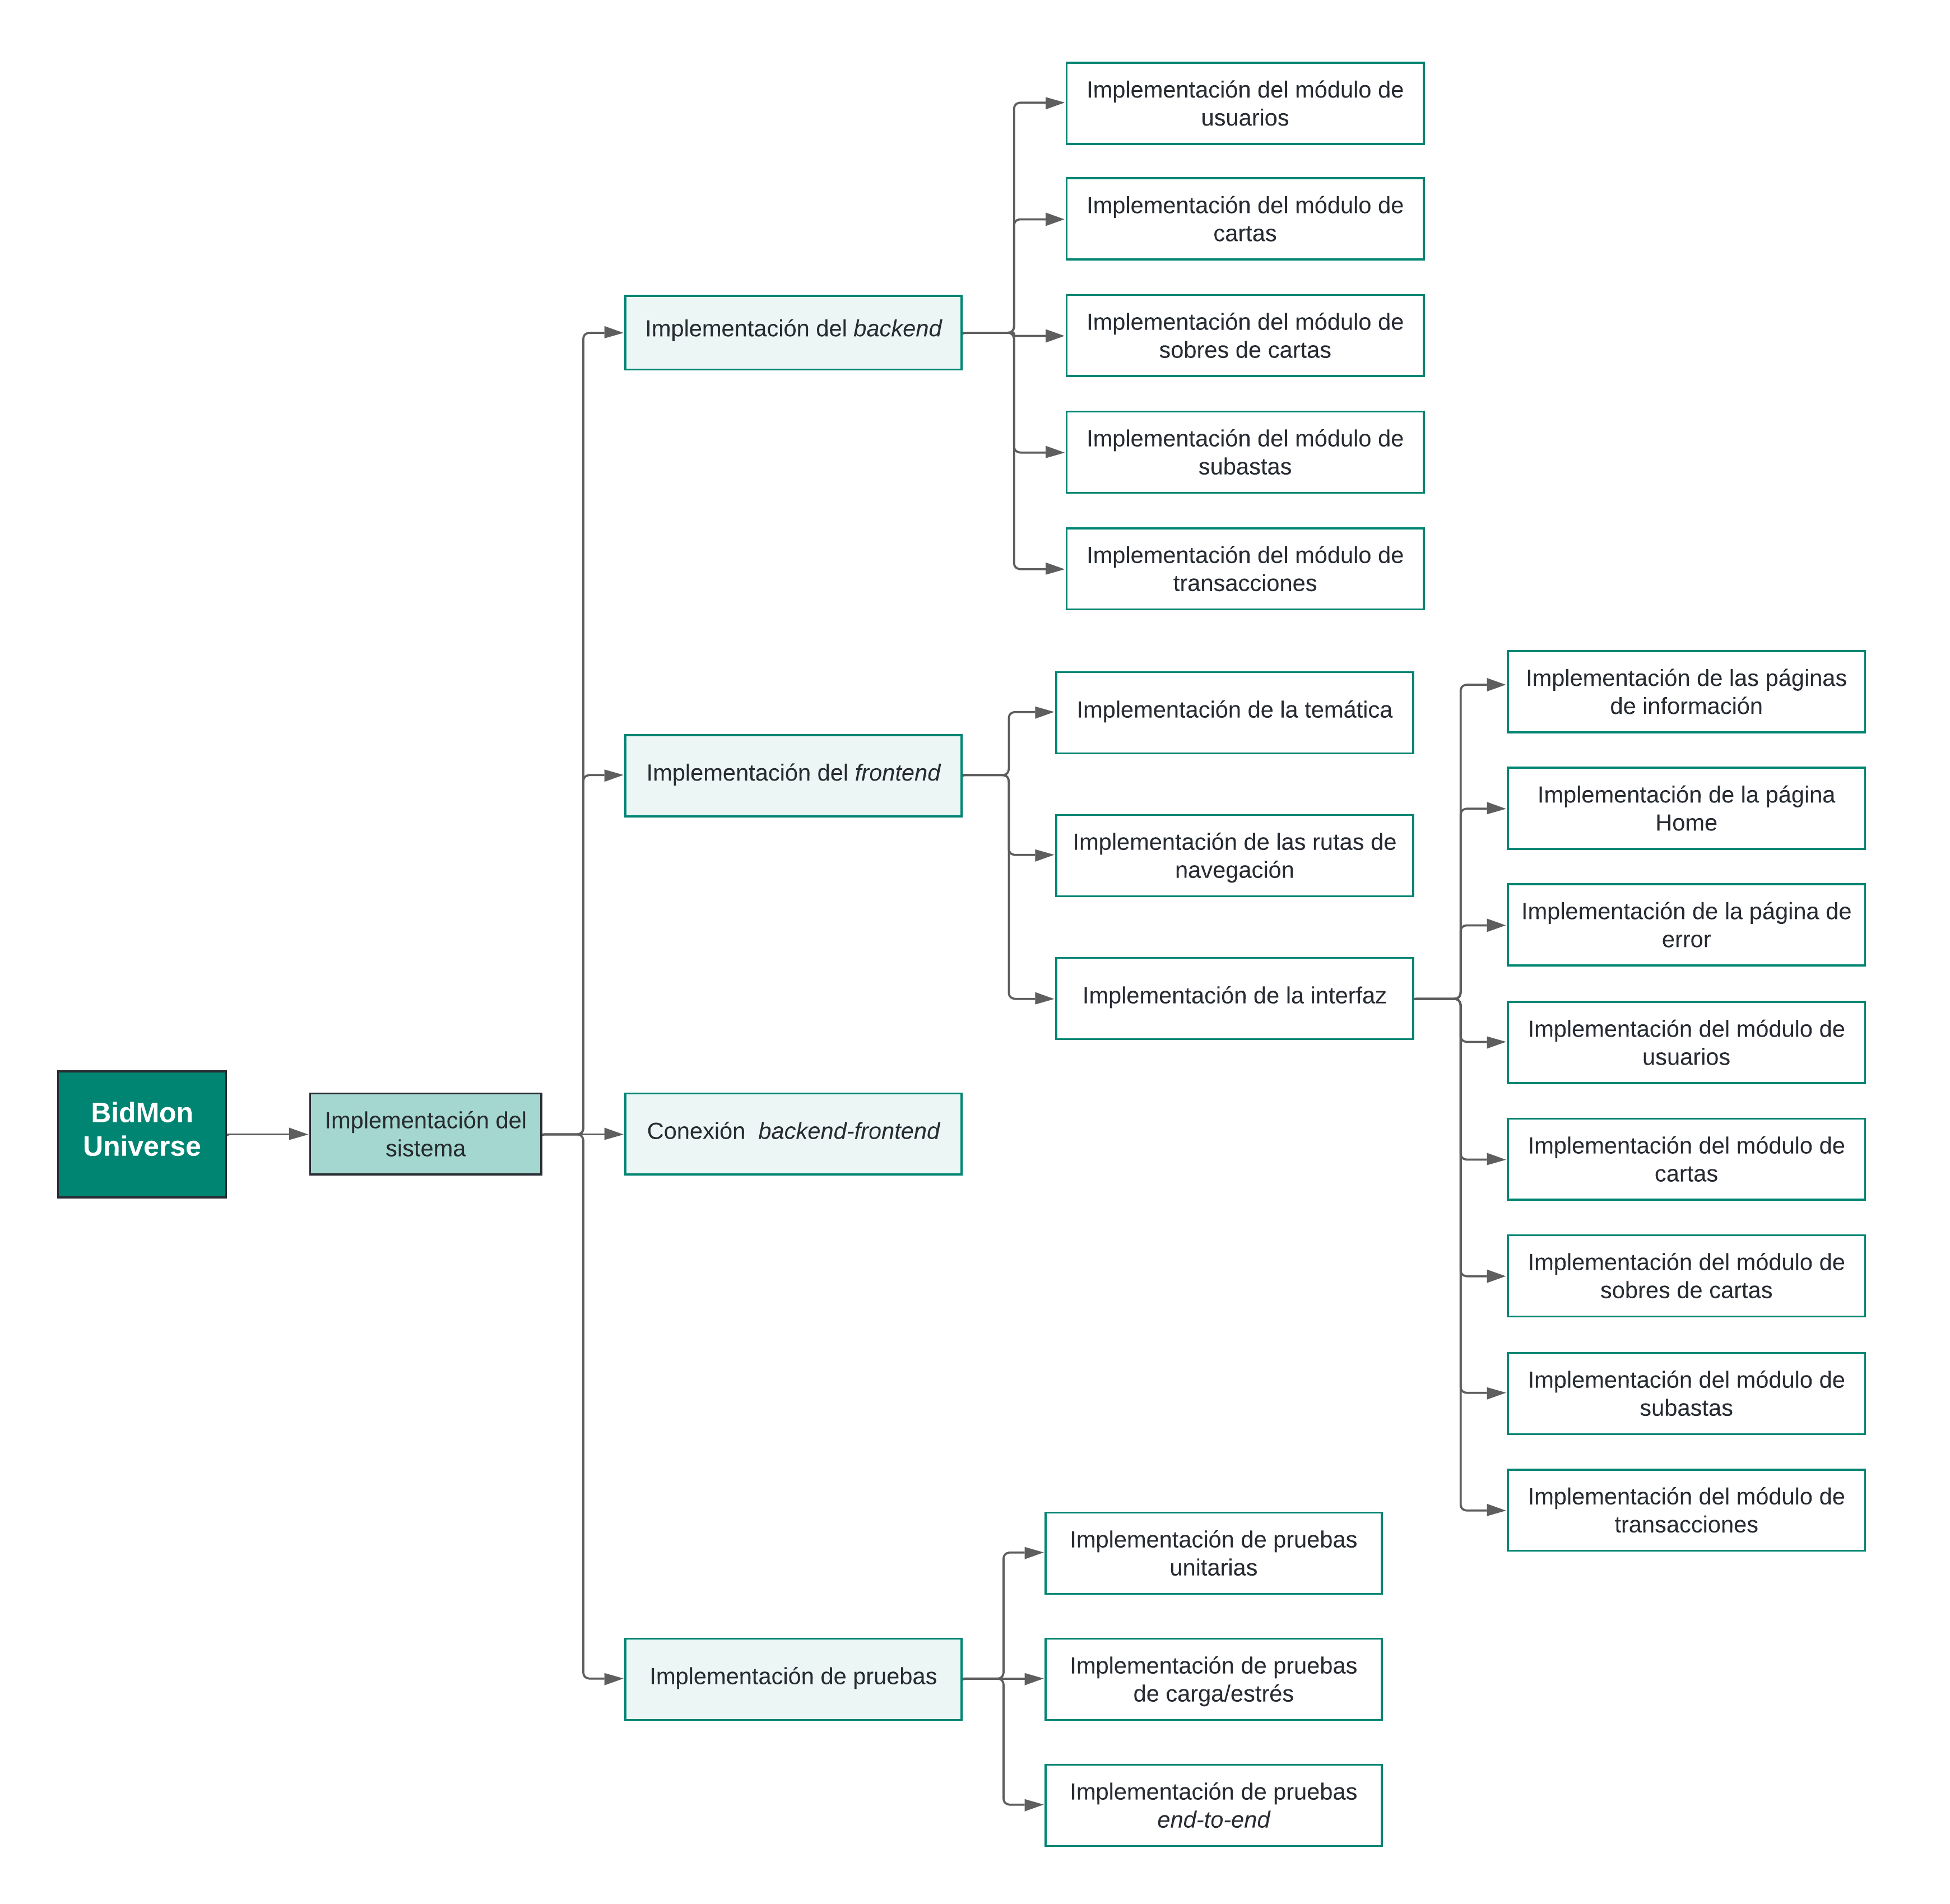
\includegraphics[width=0.9\linewidth]{figures/5-WBS/5_WBS-Implementacion.png}
    \caption{WBS. Implementación del sistema}
    \label{fig:5_WBS-Implementacion}
\end{figure}

\subsubsubsection{WBS. Fase de pruebas}
En la fase de pruebas del sistema se realizan las tareas necesarias para comprobar que el sistema cumple con los requisitos establecidos, recogiendo los informes especificados en \coloredUnderline{\hyperlink{fig:5_PBS-Pruebas}{Figura \ref*{fig:5_PBS-Pruebas}: \nameref*{fig:5_PBS-Pruebas}}}.
\begin{figure}[H]
    \hypertarget{fig:5_WBS-Pruebas}{}
    \centering
    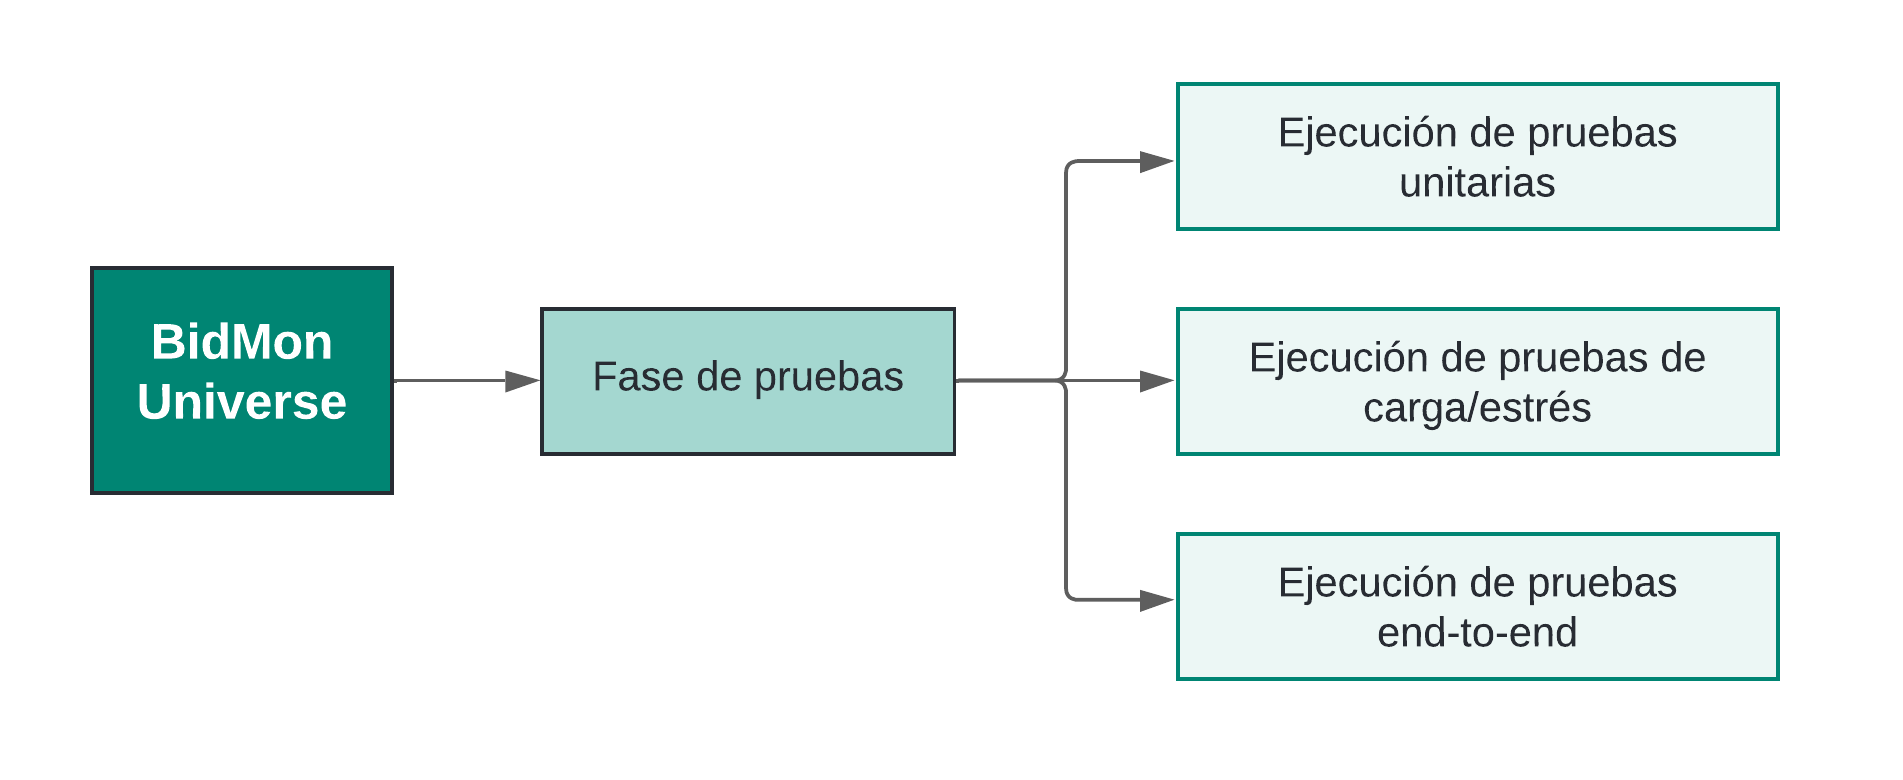
\includegraphics[width=0.9\linewidth]{figures/5-WBS/5_WBS-Pruebas.png}
    \caption{WBS. Fase de pruebas}
    \label{fig:5_WBS-Pruebas}
\end{figure}

\subsubsubsection{WBS. Despliegue del sistema}
En la fase de despliegue del sistema se realizan las tareas necesarias para poner en producción el sistema, como se detalla en la \coloredUnderline{\hyperlink{fig:5_WBS-Despliegue}{Figura \ref*{fig:5_WBS-Despliegue}: \nameref*{fig:5_WBS-Despliegue}}}.
\begin{figure}[H]
    \hypertarget{fig:5_WBS-Despliegue}{}
    \centering
    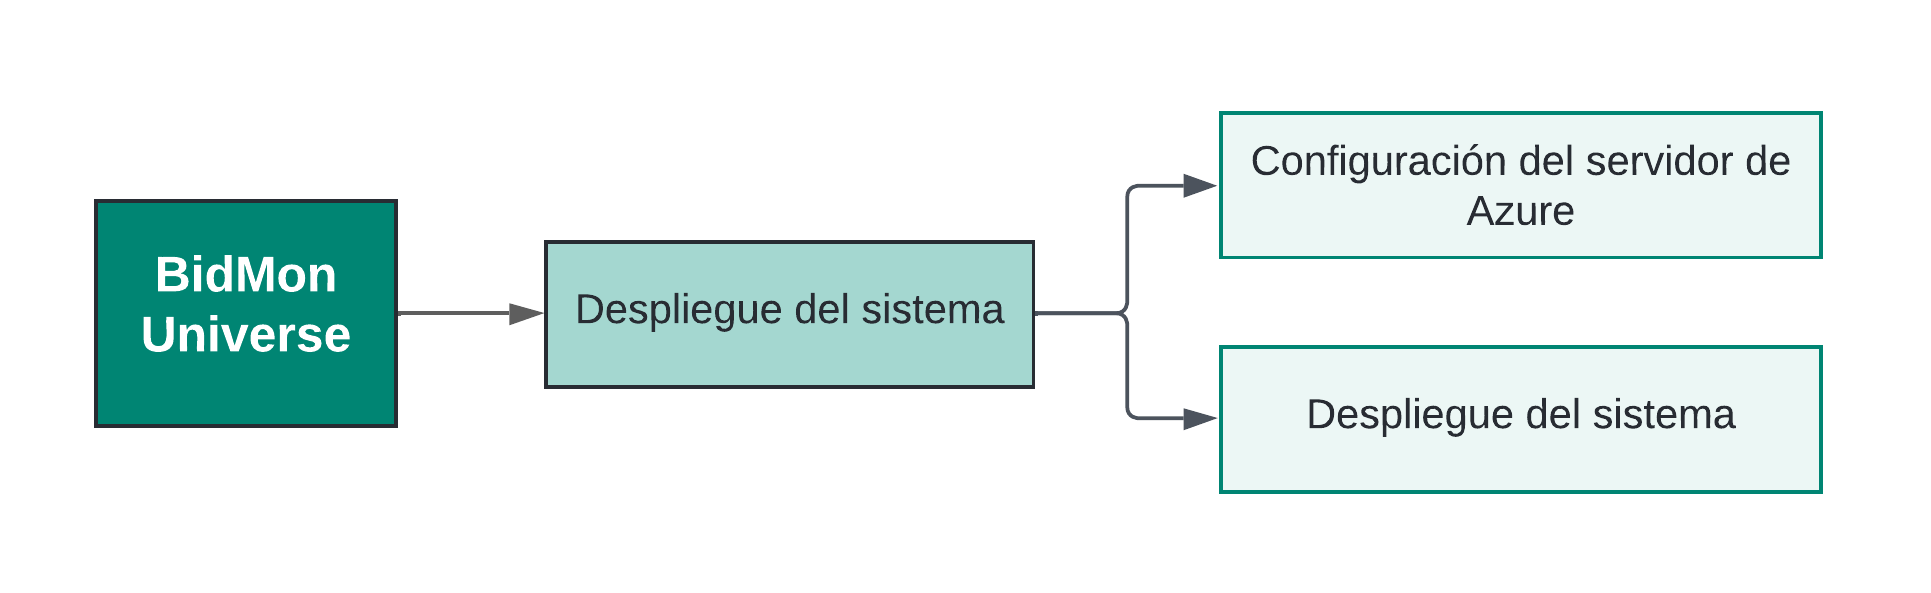
\includegraphics[width=0.9\linewidth]{figures/5-WBS/5_WBS-Despliegue2.png}
    \caption{WBS. Despliegue del sistema}
    \label{fig:5_WBS-Despliegue}
\end{figure}

\subsubsubsection{WBS. Documentación}
En la fase de documentación se realizan las tareas necesarias para la redacción de la memoria del proyecto, así como la preparación de la presentación del mismo.
\begin{figure}[H]
    \hypertarget{fig:5_WBS-Documentacion}{}
    \centering
    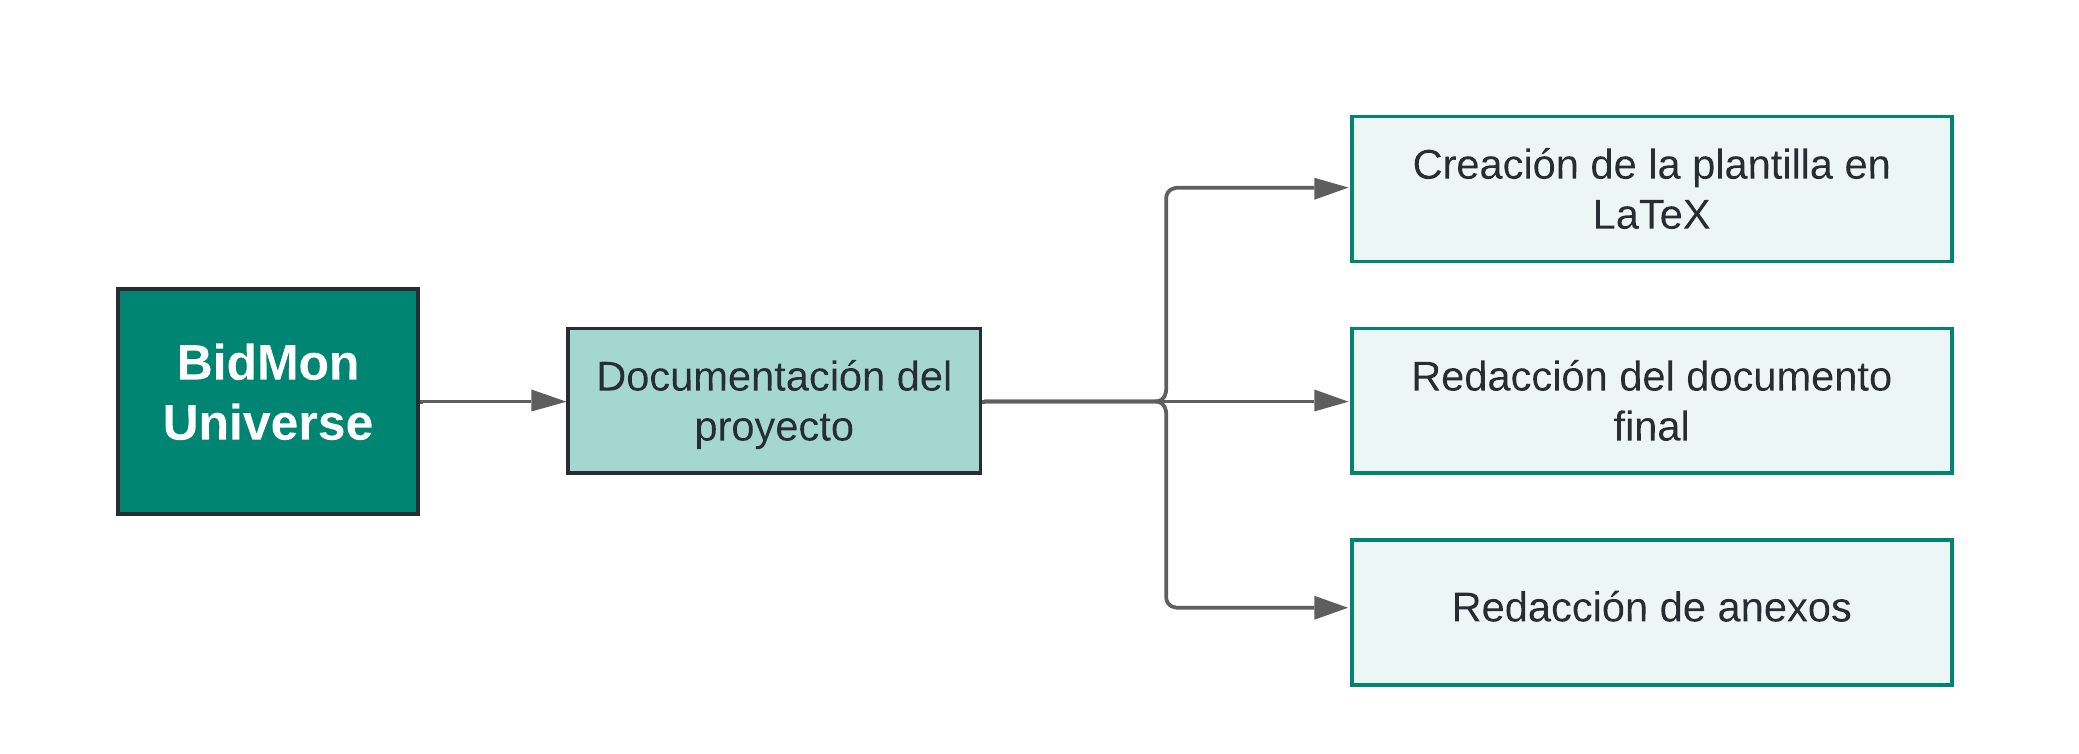
\includegraphics[width=0.9\linewidth]{figures/5-WBS/5_WBS-Documentacion.png}
    \caption{WBS. Documentación}
    \label{fig:5_WBS-Documentacion}
\end{figure}

\input{5-Planificacion-Gestion-TFG/5-Planificacion-inicial}


\subsection{Riesgos}
\subsubsection{Plan de Gestión de Riesgos} 

\subsubsection{Identificación de Riesgos}


\subsubsection{Registro de Riesgos} 

\begin{table}[htb]
    \centering
    \caption{Análisis de riesgo}
    \label{table:risk_analysis}
    \begin{tabular}{>{\columncolor{rowcolor}}l l l}
    \toprule
    \rowcolor{lightgreen}
    \textbf{Identificador} & \multicolumn{2}{l}{1} \\
    \midrule
    \textbf{Nombre} & \multicolumn{2}{l}{Problema de costos} \\
    \midrule
    \textbf{Descripción} & \multicolumn{2}{p{10cm}}{El costo de desarrollar y mantener un sitio web y un sistema de venta y distribución es alto, lo que puede afectar negativamente la rentabilidad de la empresa si no se generan suficientes ingresos para cubrir estos costos.} \\
    \midrule
    \textbf{Categoría} & \multicolumn{2}{l}{Riesgo de gestión} \\
    \midrule
    \textbf{Probabilidad} & \multicolumn{2}{l}{Media} \\
    \midrule
    \textbf{Impacto} & Presupuesto & Crítico \\
    \cmidrule(lr){2-3}
    & Planificación & Medio \\
    \cmidrule(lr){2-3}
    & Alcance & Alto \\
    \cmidrule(lr){2-3}
    & Calidad & Alto \\
    \cmidrule(lr){2-3}
    & Total & 0.45 \\
    \midrule
    \textbf{Respuesta} & \multicolumn{2}{p{10cm}}{Realizar un análisis financiero riguroso para determinar el costo total del proyecto, incluyendo los costos de desarrollo, mantenimiento, actualizaciones y otros gastos asociados. Establecer proyecciones financieras realistas para garantizar que la empresa pueda generar suficientes ingresos para cubrir estos costos y obtener una rentabilidad adecuada.} \\
    \midrule
    \textbf{Estrategia} & \multicolumn{2}{l}{Mitigar el riesgo} \\
    \bottomrule
    \end{tabular}
    \end{table}





\subsection{Presupuesto}
En esta sección se detallan los costes asociados al proyecto, incluyendo los costes de personal, materiales, licencias, infraestructura y otros gastos necesarios para la realización del proyecto.
Además, se incluye un presupuesto de cliente, que detalla los costes que el cliente deberá asumir para la realización del proyecto.


\subsubsection{Definición de la empresa} \label{sec:5-Definicion-empresa}
En esta sección se presenta la definición del modelo empresarial que ejecutará el proyecto. 
Se especificarán los costos asociados al personal que integra la empresa, así como los costos de los materiales, licencias, infraestructura y 
otros gastos necesarios para llevar a cabo las diversas actividades empresariales. 
Adicionalmente, se proporcionará un análisis de la facturación anual y los beneficios obtenidos por la empresa.

\subsubsubsection{Personal de la empresa y sueldos}
La empresa cuenta con un total de 6 personas, en el apartado \coloredUnderline{\hyperlink{sec:5-OBS}{\ref*{sec:5-OBS} \nameref*{sec:5-OBS}}}
se detalla la estructura organizativa de la empresa.
A continuación, se especifica el sueldo bruto anual de cada uno de los perfiles de la empresa, así como el coste total anual que supone el personal de la empresa.


\begin{longtable}{
    >{\raggedright\arraybackslash}p{4cm}
    >{\centering\arraybackslash}p{1.5cm}
    >{\centering\arraybackslash}p{3cm}
    >{\centering\arraybackslash}p{3cm}
    >{\centering\arraybackslash}p{3cm} }
    \caption{Costes salariales del proyecto} \label{table:costes-salariales} 
    \hypertarget{table:costes-salariales}{}
    \\

    \toprule
    \rowcolor{darkgreen!50}
    \textbf{Personal} & \textbf{Número} & \textbf{Sueldo Bruto Anual} & \textbf{Coste Salarial Anual} & \textbf{TOTAL} \\
    \midrule
    \endfirsthead

    \toprule
    \rowcolor{darkgreen!50}
    \textbf{Personal} & \textbf{Número} & \textbf{Sueldo Bruto Anual} & \textbf{Coste Salarial Anual} & \textbf{TOTAL} \\
    \midrule
    \endhead

    \midrule
    \multicolumn{5}{r}{{Continúa en la siguiente página\ldots}} \\
    \endfoot

    \bottomrule
    \endlastfoot

    \rowcolor{lightgreen!20}
    Jefe de proyecto & 1 & 30.000,00€ & 38.400,00€ & 38.400,00€ \\
    \midrule
    Analista junior & 1 & 23.000,00€ & 29.440,00€ & 29.440,00€ \\
    \midrule
    \rowcolor{lightgreen!20}
    Diseñador UX/UI junior & 1 & 21.000,00€ & 26.880,00€ & 26.880,00€ \\
    \midrule
    Desarrollador Software junior & 1 & 22.000,00€ & 28.160,00€ & 28.160,00€ \\
    \midrule
    \rowcolor{lightgreen!20}
    Tester junior & 1 & 21.000,00€ & 26.880,00€ & 26.880,00€ \\
    \midrule
    Documentador técnico & 1 & 24.500,00€ & 31.360,00€ & 31.360,00€ \\
    \midrule
    \rowcolor{lightgreen!30}
    \textbf{TOTAL} & \textbf{6} &  &  & \textbf{181.120,00€} \\
\end{longtable}


\subsubsubsection{Costes debidos a trabajos no productivos}

En la tabla \coloredUnderline{\hyperlink{table:costes-directos-indirectos}{\ref*{table:costes-directos-indirectos} \nameref*{table:costes-directos-indirectos}}} se detalla la asignación de los costes 
salariales a costes directos e indirectos. Esta asignación se debe a que no todo el tiempo de trabajo de los empleados se dedica a tareas productivas, 
también se dedica tiempo a tareas no productivas, como reuniones, formación, etc. 

La productividad se define como el porcentaje de tiempo que se dedica a tareas productivas y se calcula mediante la fórmula:

\[
\text{Productividad (R)} = \frac{\text{Cantidad de producto obtenido}}{\text{Cantidad de recurso utilizado (R)}}
\]

De esta manera, se pueden distinguir claramente los costes directos, asociados al tiempo efectivamente empleado en la producción, y los costes indirectos, correspondientes al tiempo dedicado a actividades no productivas.
En la tabla identificamos coste directo como CD y coste indirecto como CI.


\begin{longtable}{
    >{\raggedright\arraybackslash}p{4cm}
    >{\centering\arraybackslash}p{2.7cm}
    >{\centering\arraybackslash}p{1.5cm}
    >{\centering\arraybackslash}p{2.7cm}
    >{\centering\arraybackslash}p{1.5cm}
    >{\centering\arraybackslash}p{2.7cm} }
    \caption{Asignación de los costes salariales a costes directos e indirectos} \label{table:costes-directos-indirectos} 
    \hypertarget{table:costes-directos-indirectos}{}
    \\

    \toprule
    \rowcolor{darkgreen!50}
    \textbf{Personal} & \textbf{TOTAL} & \textbf{Prod. (\%)} & \textbf{CD} & \textbf{CI (\%)} & \textbf{CI} \\
    \midrule
    \endfirsthead

    \toprule
    \rowcolor{darkgreen!50}
    \textbf{Personal} & \textbf{TOTAL} & \textbf{Prod. (\%)} & \textbf{CD} & \textbf{CI (\%)} & \textbf{CI} \\
    \midrule
    \endhead

    \midrule
    \multicolumn{6}{r}{{Continúa en la siguiente página\ldots}} \\
    \endfoot

    \bottomrule
    \endlastfoot

    \rowcolor{lightgreen!20}
    Jefe de proyecto & 38.400,00€ & 0\% & 0,00€ & 100\% & 38.400,00€ \\
    \midrule
    Analista junior & 29.440,00€ & 85\% & 25.024,00€ & 15\% & 4.416,00€ \\
    \midrule
    \rowcolor{lightgreen!20}
    Diseñador UX/UI junior & 26.880,00€ & 85\% & 22.848,00€ & 15\% & 4.032,00€ \\
    \midrule
    Desarrollador Software junior & 28.160,00€ & 85\% & 23.936,00€ & 15\% & 4.224,00€ \\
    \midrule
    \rowcolor{lightgreen!20}
    Tester junior & 26.880,00€ & 85\% & 22.848,00€ & 15\% & 4.032,00€ \\
    \midrule
    Documentador técnico & 31.360,00€ & 90\% & 28.224,00€ & 10\% & 3.136,00€ \\
    \midrule
    \rowcolor{lightgreen!30}
    \textbf{TOTAL} & \textbf{181.120,00€} &  & \textbf{122.880,00€} &  & \textbf{58.240,00€} \\
\end{longtable}


Calculando las horas productivas por perfil se obtiene la tabla \coloredUnderline{\hyperlink{table:horas-productivas}{\ref*{table:horas-productivas} \nameref*{table:horas-productivas}}},
donde se obtiene el número de horas productivas por perfil y el total de horas productivas de la empresa.


\begin{longtable}{
    >{\raggedright\arraybackslash}p{4cm}
    >{\centering\arraybackslash}p{1cm}
    >{\centering\arraybackslash}p{2cm}
    >{\centering\arraybackslash}p{2cm}
    >{\centering\arraybackslash}p{3cm}
    >{\centering\arraybackslash}p{3cm} }
    \caption{Número de horas productivas por perfil y en total} \label{table:horas-productivas} 
    \hypertarget{table:horas-productivas}{}
    \\

    \toprule
    \rowcolor{darkgreen!50}
    \textbf{Personal} & \textbf{Nº} & \textbf{Prod. (\%)} & \textbf{Horas / año} & \textbf{Horas productivas / año (Por persona)} & \textbf{Horas productivas (Total empresa)} \\
    \midrule
    \endfirsthead

    \toprule
    \rowcolor{darkgreen!50}
    \textbf{Personal} & \textbf{Nº} & \textbf{Prod. (\%)} & \textbf{Horas / año} & \textbf{Horas productivas / año (Por persona)} & \textbf{Horas productivas (Total empresa)} \\
    \midrule
    \endhead

    \midrule
    \multicolumn{6}{r}{{Continúa en la siguiente página\ldots}} \\
    \endfoot

    \bottomrule
    \endlastfoot

    \rowcolor{lightgreen!20}
    Jefe de proyecto & 1 & 0\% & 2032 & 0 & 0 \\
    \midrule
    Analista junior & 1 & 80\% & 2032 & 1625,6 & 1625,6 \\
    \midrule
    \rowcolor{lightgreen!20}
    Diseñador UX/UI junior & 1 & 85\% & 2032 & 1727,2 & 1727,2 \\
    \midrule
    Desarrollador Software junior & 1 & 85\% & 2032 & 1727,2 & 1727,2 \\
    \midrule
    \rowcolor{lightgreen!20}
    Tester junior & 1 & 80\% & 2032 & 1625,6 & 1625,6 \\
    \midrule
    Documentador técnico & 1 & 90\% & 2032 & 1828,8 & 1828,8 \\
    \midrule
    \rowcolor{lightgreen!30}
    \textbf{TOTAL} & \textbf{6} &  &  &  & \textbf{8534,4} \\
\end{longtable}


\subsubsubsection{Costes de servicios}
Es necesario calcular los costes de los servicios inherentes a la empresa, estos costes se detallan en la tabla \coloredUnderline{\hyperlink{table:costes-servicios}{\ref*{table:costes-servicios} \nameref*{table:costes-servicios}}}.
Estos costes son aquellos que no están directamente relacionados con la producción, pero que son necesarios para el funcionamiento de la empresa.

\begin{longtable}{
    >{\raggedright\arraybackslash}p{7cm}
    >{\centering\arraybackslash}p{3cm}
    >{\centering\arraybackslash}p{3cm} }
    \caption{Costes de servicios} \label{table:costes-servicios} 
    \hypertarget{table:costes-servicios}{}
    \\

    \toprule
    \rowcolor{darkgreen!50}
    \textbf{Servicio} & \textbf{Coste mes} & \textbf{Coste anual} \\
    \midrule
    \endfirsthead

    \toprule
    \rowcolor{darkgreen!50}
    \textbf{Servicio} & \textbf{Coste mes} & \textbf{Coste anual} \\
    \midrule
    \endhead

    \midrule
    \multicolumn{3}{r}{{Continúa en la siguiente página\ldots}} \\
    \endfoot

    \bottomrule
    \endlastfoot

    \rowcolor{lightgreen!20}
    Alquiler de inmueble & 800,00€ & 9.600,00€ \\
    \midrule
    Tributos y tasas diversas & 650,00€ & 7.800,00€ \\
    \midrule
    \rowcolor{lightgreen!20}
    Limpieza & 500,00€ & 6.000,00€ \\
    \midrule
    Consumos de agua & 80,00€ & 960,00€ \\
    \midrule
    \rowcolor{lightgreen!20}
    Consumos de electricidad (excepto consumos para producción) & 130,00€ & 1.560,00€ \\
    \midrule
    Honorarios de asesorías, auditorías y otros profesionales & 150,00€ & 1.800,00€ \\
    \midrule
    \rowcolor{lightgreen!20}
    Primas de seguros & 600,00€ & 7.200,00€ \\
    \midrule
    Gastos en material de oficina & 50,00€ & 600,00€ \\
    \midrule
    \rowcolor{lightgreen!20}
    Gastos financieros & 200,00€ & 2.400,00€ \\
    \midrule
    \rowcolor{lightgreen!30}
    \textbf{TOTAL} & \textbf{3.160,00€} & \textbf{37.920,00€} \\
\end{longtable}


\subsubsubsection{Costes de los medios de producción}
Por otro lado, es necesario calcular los costes de los medios de producción, estos costes se detallan en la tabla \coloredUnderline{\hyperlink{table:costes-medios-produccion}{\ref*{table:costes-medios-produccion} \nameref*{table:costes-medios-produccion}}}.
Estos costes son aquellos que están directamente relacionados con la producción, como los costes de los equipos informáticos, licencias de software, etc.

Estos costes se han clasificado en dos tipos: costes de amortización y costes de alquiler. Los costes de amortización son aquellos que se pagan de una sola vez y se amortizan a lo largo de varios años, 
mientras que los costes de alquiler son aquellos que se pagan de forma periódica. Para los costes de amortización se ha calculado el coste anual de amortización y el plazo de amortización en años.

En la tabla identificamos coste anual como CA y coste total como CT

\begin{longtable}{
    >{\raggedright\arraybackslash}p{2cm}
    >{\raggedright\arraybackslash}p{3.7cm}
    >{\centering\arraybackslash}p{0.5cm}
    >{\centering\arraybackslash}p{2cm}
    >{\centering\arraybackslash}p{2cm}
    >{\centering\arraybackslash}p{2cm}
    >{\centering\arraybackslash}p{2cm}
    >{\centering\arraybackslash}p{1.5cm} }
    \caption{Costes de los medios de producción} \label{table:costes-medios-produccion} 
    \hypertarget{table:costes-medios-produccion}{}
    \\

    \toprule
    \rowcolor{darkgreen!50}
    \textbf{Equipo / Licencia} & \textbf{Características} & \textbf{ud.} & \textbf{Precio} & \textbf{CT} & \textbf{CA} & \textbf{Tipo} & \textbf{Plazo} \\
    \midrule
    \endfirsthead

    \toprule
    \rowcolor{darkgreen!50}
    \textbf{Equipo / Licencia} & \textbf{Características} & \textbf{ud.} & \textbf{Precio} & \textbf{CT} & \textbf{CA} & \textbf{Tipo} & \textbf{Plazo} \\
    \midrule
    \endhead

    \midrule
    \multicolumn{8}{r}{{Continúa en la siguiente página\ldots}} \\
    \endfoot

    \bottomrule
    \endlastfoot

    \rowcolor{lightgreen!20}
    Portátiles & MacBook Pro 16 pulgadas Chip M3 Max de Apple con CPU de 14 núcleos, GPU de 30 núcleos y Neural Engine de 16 núcleos, 36GB memoria unificada, 1TB de almacenamiento SSD & 1 & 4.299,00€ & 4.299,00€ & 1.074,75€ & Amortizac. & 4 \\
    \midrule
    Portátiles & Portátil HP Pavilion Plus 16-ab0004ns, Windows 11 Home, Intel\textregistered{} Core\texttrademark{} i7 13700H (13.ª generación), 16 GB RAM, 1 TB SSD, 16 pulgadas, WQXGA (2560 x 1600), 120 Hz, NVIDIA\textregistered{} GeForce RTX\texttrademark{} 3050 (6 GB) & 5 & 1.499,00€ & 7.495,00€ & 1.873,75€ & Amortizac. & 4 \\
    \midrule
    \rowcolor{lightgreen!20}
    Licencia Overleaf & Licencia \textit{Group Standard} para 10 usuarios & 1 & 1.160,00€ & 1.160,00€ & 1.160,00€ & Alquiler & - \\
    \midrule
    Licencia Excalidraw & Licencia Anual & 2 & 72,00€ & 144,00€ & 144,00€ & Alquiler & - \\
    \midrule
    \rowcolor{lightgreen!20}
    Licencia Office 365 & Microsoft 365 Plan Empresa Premium & 6 & 247,20€ & 1.483,20€ & 1.483,20€ & Alquiler & - \\
    \midrule
    Licencia MS Project & Compra de pago único Project Profesional 2021 & 1 & 1.659,00€ & 1.659,00€ & 331,80€ & Amortizac. & 5 \\
    \midrule
    \rowcolor{lightgreen!20}
    Conexión a internet & Fibra 600 MB con centralita virtual & 1 & 1.013,76€ & 1.013,76€ & 1.013,76€ & Alquiler & - \\
    \midrule
    \rowcolor{lightgreen!30}
    \textbf{TOTAL} &  &  &  & \textbf{7.081,26€} &  &  &  \\
\end{longtable}



\subsubsubsection{Precio por hora de trabajo y facturación total de la empresa}
En la tabla \coloredUnderline{\hyperlink{table:precios-facturacion}{\ref*{table:precios-facturacion} \nameref*{table:precios-facturacion}}} se detalla el precio por hora de trabajo de cada uno de los perfiles de la empresa,
así como el total de horas productivas de la empresa y la facturación total de la empresa.

Este precio por hora permite cubrir los costes salariales, los costes de servicios y los costes de los medios de producción, así como obtener un beneficio para la empresa.

La facturación total de la empresa se calcula multiplicando el precio por hora de trabajo de cada perfil por el número de horas productivas de cada perfil y sumando el total de horas productivas de la empresa,
con lo que se obtiene que la empresa facturará un total de 230.530,40€ al año.

\begin{longtable}{
    >{\raggedright\arraybackslash}p{5cm}
    >{\centering\arraybackslash}p{3cm}
    >{\centering\arraybackslash}p{4cm}
    >{\centering\arraybackslash}p{4cm} }
    \caption{Precios por hora de trabajo y facturación total de la empresa} \label{table:precios-facturacion} 
    \hypertarget{table:precios-facturacion}{}
    \\

    \toprule
    \rowcolor{darkgreen!50}
    \textbf{Personal} & \textbf{Precio/hora} & \textbf{Horas productivas (Total empresa)} & \textbf{Facturación} \\
    \midrule
    \endfirsthead

    \toprule
    \rowcolor{darkgreen!50}
    \textbf{Personal} & \textbf{Precio/hora} & \textbf{Horas productivas (Total empresa)} & \textbf{Facturación} \\
    \midrule
    \endhead

    \midrule
    \multicolumn{4}{r}{{Continúa en la siguiente página\ldots}} \\
    \endfoot

    \bottomrule
    \endlastfoot

    \rowcolor{lightgreen!20}
    Jefe de proyecto & 40,00€ & 0,00 & 0,00€ \\
    \midrule
    Analista junior & 30,00€ & 1625,60 & 48.768,00€ \\
    \midrule
    \rowcolor{lightgreen!20}
    Diseñador UX/UI junior & 26,00€ & 1727,20 & 44.907,20€ \\
    \midrule
    Desarrollador Software junior & 25,00€ & 1727,20 & 43.180,00€ \\
    \midrule
    \rowcolor{lightgreen!20}
    Tester junior & 25,00€ & 1625,60 & 40.640,00€ \\
    \midrule
    Documentador técnico & 29,00€ & 1828,80 & 53.035,20€ \\
    \midrule
    \rowcolor{lightgreen!30}
    \textbf{TOTAL} &  & \textbf{8534,40} & \textbf{230.530,40€} \\
\end{longtable}



\subsubsubsection{Precio por hora a usar para el cálculo de los proyectos de costes}
En la tabla \coloredUnderline{\hyperlink{table:precio-hora}{\ref*{table:precio-hora} \nameref*{table:precio-hora}}} se detalla el precio por hora a usar para el cálculo de los proyectos de costes.
Este es el precio real que la empresa tiene que pagar por hora de trabajo de cada uno de los perfiles de la empresa.


\begin{longtable}{
    >{\raggedright\arraybackslash}p{5cm}
    >{\centering\arraybackslash}p{3cm} }
    \caption{Precio por hora a usar para el cálculo de los proyectos de costes} \label{table:precio-hora} 
    \hypertarget{table:precio-hora}{}
    \\

    \toprule
    \rowcolor{darkgreen!50}
    \textbf{Personal} & \textbf{Precio/hora} \\
    \midrule
    \endfirsthead

    \toprule
    \rowcolor{darkgreen!50}
    \textbf{Personal} & \textbf{Precio/hora} \\
    \midrule
    \endhead

    \midrule
    \multicolumn{2}{r}{{Continúa en la siguiente página\ldots}} \\
    \endfoot

    \bottomrule
    \endlastfoot

    \rowcolor{lightgreen!20}
    Jefe de proyecto & 18,90€ \\
    \midrule
    Analista junior & 14,49€ \\
    \midrule
    \rowcolor{lightgreen!20}
    Diseñador UX/UI junior & 13,23€ \\
    \midrule
    Desarrollador Software junior & 13,86€ \\
    \midrule
    \rowcolor{lightgreen!20}
    Tester junior & 13,23€ \\
    \midrule
    Documentador técnico & 15,43€ \\
\end{longtable}



\subsubsubsection{Resumen del modelo de empresa}
Tras los cálculos realizados, se obtiene el resumen del modelo de empresa, que se detalla en la tabla \coloredUnderline{\hyperlink{table:resumen-modelo-empresa}{\ref*{table:resumen-modelo-empresa} \nameref*{table:resumen-modelo-empresa}}}.
En esta tabla se detalla el total de los costes directos, el total de los costes indirectos, la suma de los costes directos e indirectos, el beneficio deseado, el coste total, 
la facturación posible en función de las horas de producción y de los precios por hora calculados, y el margen entre el coste total y la facturación.

La empresa obtiene un margen del 2,034\% entre el coste total y la facturación, lo que indica que la empresa obtiene un beneficio del 2,034\% sobre el coste total.

\begin{longtable}{
    >{\centering\arraybackslash}p{1cm}
    >{\raggedright\arraybackslash}p{8cm}
    >{\centering\arraybackslash}p{4cm} }
    \caption{Resumen del modelo de empresa} \label{table:resumen-modelo-empresa} 
    \hypertarget{table:resumen-modelo-empresa}{}
    \\

    \toprule
    \rowcolor{darkgreen!50}
    \textbf{Nº} & \textbf{Concepto} & \textbf{Importe} \\
    \midrule
    \endfirsthead

    \toprule
    \rowcolor{darkgreen!50}
    \textbf{Nº} & \textbf{Concepto} & \textbf{Importe} \\
    \midrule
    \endhead

    \midrule
    \multicolumn{3}{r}{{Continúa en la siguiente página\ldots}} \\
    \endfoot

    \bottomrule
    \endlastfoot

    \rowcolor{lightgreen!20}
    1 & Total de los costes directos & 122.880,00€ \\
    \midrule
    2 & Total de los costes indirectos & 65.321,26€ \\
    \midrule
    \rowcolor{lightgreen!20}
    3 & Suma de los costes directos e indirectos & 188.201,26€ \\
    \midrule
    4 & Beneficio deseado (20\%) & 37.640,25€ \\
    \midrule
    \rowcolor{lightgreen!20}
    5 & Coste total (suma de los costes directos, indirectos y beneficios) & 225.841,51€ \\
    \midrule
    6 & Facturación posible en función de las horas de producción y de los precios por hora calculados & 230.530,40€ \\
    \midrule
    \rowcolor{lightgreen!20}
    7 & Margen entre el coste total y la facturación (relación entre 5 y 6) & 2,034\% \\
\end{longtable}




\subsubsection{Presupuesto de Costes}
En esta sección se presentará el presupuesto de costes.

En primer lugar, se presentará un resumen de la cuantía total necesaria para llevar a cabo el proyecto, ver \coloredUnderline{\hyperlink{table:partidas-proyecto}{Tabla \ref*{table:partidas-proyecto}: \nameref*{table:partidas-proyecto}}}
, y a continuación se detallarán los presupuestos de cada una de las partidas que lo componen.

La cuantía total necesaria para llevar a cabo el proyecto asciende a \textbf{6.738,36€}. 



\begin{longtable}{
    >{\centering\arraybackslash}p{0.5cm}
    >{\raggedright\arraybackslash}p{5cm}
    >{\centering\arraybackslash}p{3cm} }
    \caption{Resumen presupuesto de costes del proyecto} \label{table:partidas-proyecto} \\
    \hypertarget{table:partidas-proyecto}{}
    \\

    \toprule
    \rowcolor{darkgreen!50}
    \textbf{Nº} & \textbf{Nombre de la partida} & \textbf{Total} \\
    \midrule
    \endfirsthead

    \toprule
    \rowcolor{darkgreen!50}
    \textbf{Nº} & \textbf{Nombre de la partida} & \textbf{Total} \\
    \midrule
    \endhead

    \midrule
    \multicolumn{3}{r}{{Continúa en la siguiente página\ldots}} \\
    \endfoot

    \bottomrule
    \endlastfoot

    \rowcolor{lightgreen!20}
    1 & Análisis del sistema & 173,54€ \\
    \midrule
    \rowcolor{lightgreen!10}
    2 & Seguimiento del proyecto & 478,27€ \\
    \midrule
    \rowcolor{lightgreen!20}
    3 & Diseño del sistema & 1.023,75€ \\
    \midrule
    \rowcolor{lightgreen!10}
    4 & Implementación del sistema & 2.158,17€ \\
    \midrule
    \rowcolor{lightgreen!20}
    5 & Fase de pruebas & 136,85€ \\
    \midrule
    \rowcolor{lightgreen!10}
    6 & Despliegue del sistema & 144,16€ \\
    \midrule
    \rowcolor{lightgreen!20}
    7 & Documentación del proyecto & 2.623,62€ \\
    \midrule
    \rowcolor{lightgreen!30}
    & \textbf{TOTAL} & \textbf{6.738,36€} \\
\end{longtable}


%--- PARTIDA 1: ANÁLISIS DEL PROYECTO ---
\begin{longtable}{
    >{\centering\arraybackslash}p{0.5cm}
    >{\centering\arraybackslash}p{0.5cm}
    >{\raggedright\arraybackslash}p{5cm}
    >{\centering\arraybackslash}p{1.5cm}
    >{\centering\arraybackslash}p{1.5cm}
    >{\centering\arraybackslash}p{1.5cm}
    >{\centering\arraybackslash}p{2.5cm}
    >{\centering\arraybackslash}p{2cm} }
    \caption{Presupuesto Inicial. Partida 1: Análisis del proyecto} \label{table:5_Presupuesto-P1-Analisis} \\
    \hypertarget{table:5_Presupuesto-P1-Analisis}{}
    \\

    \toprule
    \rowcolor{darkgreen!50}
    \textbf{I1} & \textbf{I2} & \textbf{Descripción} & \textbf{Cant.} & \textbf{ud.} & \textbf{Precio} & \textbf{Subtotal (2)} & \textbf{Total} \\
    \midrule
    \endfirsthead

    \toprule
    \rowcolor{darkgreen!50}
    \textbf{I1} & \textbf{I2} & \textbf{Descripción} & \textbf{Cant.} & \textbf{ud.} & \textbf{Precio} & \textbf{Subtotal} & \textbf{Total} \\
    \midrule
    \endhead

    \midrule
    \multicolumn{8}{r}{{Presupuesto Inicial. Partida 1: Análisis del proyecto -- Continúa en la siguiente página\ldots}} \\
    \endfoot

    \bottomrule
    \endlastfoot
    \rowcolor{lightgreen!30}
    1 &  & Análisis del sistema &  &  &  &  & 72,44€ \\
    \midrule
    & 1 & Analista junior & 5 & horas & 14,49€ & 72,44€ &  \\
    \midrule
    \rowcolor{lightgreen!30}
    2 &  & Análisis de la Arquitectura &  &  &  &  & 43,46€ \\
    \midrule
    & 1 & Analista junior & 3 & horas & 14,49€ & 43,46€ &  \\
    \midrule
    \rowcolor{lightgreen!30}
    3 &  & Análisis de la Infraestructura &  &  &  &  & 28,98€ \\
    \midrule
    & 1 & Analista junior & 2 & horas & 14,49€ & 28,98€ &  \\
    \midrule
    \rowcolor{lightgreen!30}
    4 &  & Determinación del alcance de desarrollo &  &  &  &  & 28,66€ \\
    \midrule
    & 1 & Desarrollador Software junior & 0,5 & horas & 13,86€ & 6,93€ &  \\
    \midrule
    & 2 & Analista junior & 1,5 & horas & 14,49€ & 21,73€ &  \\
    \midrule
    &  &  &  &  &  & \textbf{TOTAL:} & \textbf{173,54€} \\
\end{longtable}




%----- PARTIDA 2: SEGUIMIENTO DEL SISTEMA -----

\begin{longtable}{
    >{\centering\arraybackslash}p{0.5cm}
    >{\centering\arraybackslash}p{0.5cm}
    >{\raggedright\arraybackslash}p{5cm}
    >{\centering\arraybackslash}p{1.5cm}
    >{\centering\arraybackslash}p{1.5cm}
    >{\centering\arraybackslash}p{1.5cm}
    >{\centering\arraybackslash}p{2.5cm}
    >{\centering\arraybackslash}p{2cm} }
    \caption{Presupuesto Inicial. Partida 2: Seguimiento del sistema} \label{table:5_Presupuesto-P2-Seguimiento} \\
    \hypertarget{table:5_Presupuesto-P1-Analisis}{}
    \\

    \toprule
    \rowcolor{darkgreen!50}
    \textbf{I1} & \textbf{I2} & \textbf{Descripción} & \textbf{Cant.} & \textbf{ud.} & \textbf{Precio} & \textbf{Subtotal (2)} & \textbf{Total} \\
    \midrule
    \endfirsthead

    \toprule
    \rowcolor{darkgreen!50}
    \textbf{I1} & \textbf{I2} & \textbf{Descripción} & \textbf{Cant.} & \textbf{ud.} & \textbf{Precio} & \textbf{Subtotal} & \textbf{Total} \\
    \midrule
    \endhead

    \midrule
    \multicolumn{8}{r}{{Presupuesto Inicial. Partida 2: Seguimiento del sistema -- Continúa en la siguiente página\ldots}} \\
    \endfoot

    \bottomrule
    \endlastfoot
    \rowcolor{lightgreen!30}
    1 &  & Reunión de arranque &  &  &  &  & 30,39€ \\
    \midrule
    & 1 & Documentador técnico & 1,5 & horas & 15,43€ & 23,15€ &  \\
    \midrule
    & 2 & Analista junior & 0,5 & horas & 14,49€ & 7,24€ &  \\
    \midrule
    \rowcolor{lightgreen!30}
    2 &  & Reuniones periódicas &  &  &  &  & 299,84€ \\
    \midrule
    & 1 & Documentador técnico & 10 & horas & 15,43€ & 154,33€ &  \\
    \midrule
    & 2 & Desarrollador Software junior & 10,5 & horas & 13,86€ & 145,51€ &  \\
    \midrule
    \rowcolor{lightgreen!30}
    4 &  & Reunión de revisión &  &  &  &  & 89,45€ \\
    \midrule
    & 1 & Documentador técnico & 2 & horas & 15,43€ & 30,87€ &  \\
    \midrule
    & 2 & Desarrollador Software junior & 2 & horas & 13,86€ & 27,72€ &  \\
    \midrule
    \rowcolor{lightgreen!30}
    4 &  & Reunión final &  &  &  &  & 58,58€ \\
    \midrule
    & 1 & Documentador técnico & 2 & horas & 15,43€ & 30,87€ &  \\
    \midrule
    & 2 & Desarrollador Software junior & 2 & horas & 13,86€ & 27,72€ &  \\
    \midrule
    &  &  &  &  &  & \textbf{TOTAL:} & \textbf{478,27€} \\
\end{longtable}

%----- PARTIDA 3: DISEÑO DEL SISTEMA -----
\begin{landscape}
  
    \begin{longtable}{
    >{\centering\arraybackslash}p{0.3cm}
    >{\centering\arraybackslash}p{0.3cm}
    >{\centering\arraybackslash}p{0.3cm}
    >{\centering\arraybackslash}p{0.3cm}
    >{\raggedright\arraybackslash}p{5cm}
    >{\centering\arraybackslash}p{1.2cm}
    >{\centering\arraybackslash}p{1.2cm}
    >{\centering\arraybackslash}p{1.5cm}
    >{\centering\arraybackslash}p{1.5cm}
    >{\centering\arraybackslash}p{1.5cm}
    >{\centering\arraybackslash}p{1.5cm}
    >{\centering\arraybackslash}p{2cm} }
    \caption{Planificación final. Diseño del sistema} \label{table:5_Presupuesto-P3-Diseno} \\
    \hypertarget{table:5_Presupuesto-P3-Diseno}{}
    \\

    \toprule
    \rowcolor{darkgreen!50}
    \textbf{I1} & \textbf{I2} & \textbf{I3} & \textbf{I4} & \textbf{Descripción} & \textbf{Cant.} & \textbf{ud.} & \textbf{Precio} & \textbf{Subt. 4} & \textbf{Subt. 3} & \textbf{Subt. 2} & \textbf{Total} \\
    \midrule
    \endfirsthead

    \toprule
    \rowcolor{darkgreen!50}
    \textbf{I1} & \textbf{I2} & \textbf{I3} & \textbf{I4} & \textbf{Descripción} & \textbf{Cant.} & \textbf{ud.} & \textbf{Precio} & \textbf{Subt. 4} & \textbf{Subt. 3} & \textbf{Subt. 2} & \textbf{Total} \\
    \midrule
    \endhead

    \midrule
    \multicolumn{12}{r}{{Planificación final. Diseño del sistema -- Continúa en la siguiente página\ldots}} \\
    \endfoot

    \bottomrule
    \endlastfoot

    \rowcolor{lightgreen!30}
    1 &  &  &  & Diseño del backend &  &  &  &  &  &  & 304,88€ \\
    \midrule
    \rowcolor{lightgreen!15}
    & 1 &  &  & Diseño del módulo de usuarios &  &  &  &  &  & 304,88€ &  \\
    \midrule
    &  & 1 &  & Desarrollador Software junior & 2 & horas & 13,86€ &  &  & 27,72€ &  \\
    \midrule
    \rowcolor{lightgreen!15}
    & 2 &  &  & Diseño del módulo de cartas &  &  &  &  &  &  &  \\
    \midrule
    &  & 1 &  & Desarrollador Software junior & 6 & horas & 13,86€ &  &  & 83,15€ &  \\
    \midrule
    \rowcolor{lightgreen!15}
    & 3 &  &  & Diseño del módulo de sobres de cartas &  &  &  &  &  &  &  \\
    \midrule
    &  & 1 &  & Desarrollador Software junior & 3 & horas & 13,86€ &  &  & 41,57€ &  \\
    \midrule
    \rowcolor{lightgreen!15}
    & 4 &  &  & Diseño del módulo de subastas &  &  &  &  &  &  &  \\
    \midrule
    &  & 1 &  & Desarrollador Software junior & 6.5 & horas & 13,86€ &  &  & 90,08€ &  \\
    \midrule
    \rowcolor{lightgreen!15}
    & 5 &  &  & Diseño del módulo de transacciones &  &  &  &  &  &  &  \\
    \midrule
    &  & 1 &  & Desarrollador Software junior & 4.5 & horas & 13,86€ &  &  & 62,36€ &  \\
    \midrule

    \rowcolor{lightgreen!30}
    2 &  &  &  & Diseño del frontend &  &  &  &  &  &  & 479,81€ \\
    \midrule
    \rowcolor{lightgreen!15}
    & 1 &  &  & Diseño de elementos gráficos &  &  &  &  &  &  & 39,69€ \\
    \midrule
    &  & 1 &  & Diseño de la moneda de la aplicación & 1 & horas & 13,23€ & 13,23€ &  &  &  \\
    \midrule
    &  & 2 &  & Diseño del logo de la aplicación & 2 & horas & 13,23€ & 26,46€ &  &  &  \\
    \midrule
    \rowcolor{lightgreen!15}
    & 2 &  &  & Diseño de la temática &  &  &  &  & 26,46€ &  &  \\
    \midrule
    &  & 1 &  & Diseñador UX/UI junior & 2 & horas & 13,23€ &  &  & 26,46€ &  \\
    \midrule
    \rowcolor{lightgreen!15}
    & 3 &  &  & Diseño del árbol de navegación &  &  &  &  & 26,46€ &  &  \\
    \midrule
    &  & 1 &  & Diseñador UX/UI junior & 2 & horas & 13,23€ &  &  & 26,46€ &  \\
    \midrule
    \rowcolor{lightgreen!15}
    & 4 &  &  & Diseño de la interfaz de usuario &  &  &  &  &  & 387,21€ &  \\
    \midrule
    &  & 1 &  & Diseño de las páginas de información &  &  &  &  & 40,00€ &  &  \\
    \midrule
    &  &  & 1 & Diseñador UX/UI junior & 2.5 & horas & 13,23€ & 33,07€ &  &  &  \\
    \midrule
    &  &  & 2 & Desarrollador Software junior & 0.5 & horas & 13,86€ & 6,93€ &  &  &  \\
    \midrule
    &  & 2 &  & Diseño de la página Home &  &  &  &  & 53,23€ &  &  \\
    \midrule
    &  &  & 1 & Diseñador UX/UI junior & 3.5 & horas & 13,23€ & 46,30€ &  &  &  \\
    \midrule
    &  &  & 2 & Desarrollador Software junior & 0.5 & horas & 13,86€ & 6,93€ &  &  &  \\
    \midrule
    &  & 3 &  & Diseño de la página de error &  &  &  &  & 13,35€ &  &  \\
    \midrule
    &  &  & 1 & Diseñador UX/UI junior & 0.8 & horas & 13,23€ & 10,58€ &  &  &  \\
    \midrule
    &  &  & 2 & Desarrollador Software junior & 0.2 & horas & 13,86€ & 2,77€ &  &  &  \\
    \midrule
    &  & 4 &  & Diseño del módulo de usuarios &  &  &  &  & 73,39€ &  &  \\
    \midrule
    &  &  & 1 & Diseñador UX/UI junior & 4.5 & horas & 13,23€ & 59,53€ &  &  &  \\
    \midrule
    &  &  & 2 & Desarrollador Software junior & 1 & horas & 13,86€ & 13,86€ &  &  &  \\
    \midrule
    &  & 5 &  & Diseño del módulo de cartas &  &  &  &  & 53,54€ &  &  \\
    \midrule
    &  &  & 1 & Diseñador UX/UI junior & 3 & horas & 13,23€ & 39,69€ &  &  &  \\
    \midrule
    &  &  & 2 & Desarrollador Software junior & 1 & horas & 13,86€ & 13,86€ &  &  &  \\
    \midrule
    &  & 6 &  & Diseño del módulo de sobres de cartas &  &  &  &  & 26,77€ &  &  \\
    \midrule
    &  &  & 1 & Diseñador UX/UI junior & 1.5 & horas & 13,23€ & 19,84€ &  &  &  \\
    \midrule
    &  &  & 2 & Desarrollador Software junior & 0.5 & horas & 13,86€ & 6,93€ &  &  &  \\
    \midrule
    &  & 7 &  & Diseño del módulo de subastas &  &  &  &  & 73,39€ &  &  \\
    \midrule
    &  &  & 1 & Diseñador UX/UI junior & 4.5 & horas & 13,23€ & 59,53€ &  &  &  \\
    \midrule
    &  &  & 2 & Desarrollador Software junior & 1 & horas & 13,86€ & 13,86€ &  &  &  \\
    \midrule
    &  & 8 &  & Diseño del módulo de transacciones &  &  &  &  & 53,54€ &  &  \\
    \midrule
    &  &  & 1 & Diseñador UX/UI junior & 3 & horas & 13,23€ & 39,69€ &  &  &  \\
    \midrule
    &  &  & 2 & Desarrollador Software junior & 1 & horas & 13,86€ & 13,86€ &  &  &  \\
    \midrule

    \rowcolor{lightgreen!30}
    3 &  &  &  & Diseño de pruebas &  &  &  &  &  &  & 239,06€ \\
    \midrule
    \rowcolor{lightgreen!15}
    & 1 &  &  & Diseño de pruebas unitarias &  &  &  &  &  & 86,30€ &  \\
    \midrule
    &  & 1 &  & Tester junior & 6 & horas & 13,23€ & 79,37€ &  &  &  \\
    \midrule
    &  & 2 &  & Desarrollador Software junior & 0.5 & horas & 13,86€ & 6,93€ &  &  &  \\
    \midrule
    \rowcolor{lightgreen!15}
    & 2 &  &  & Diseño de las pruebas de carga/estrés &  &  &  &  &  & 66,46€ &  \\
    \midrule
    &  & 1 &  & Tester junior & 4.5 & horas & 13,23€ & 59,53€ &  &  &  \\
    \midrule
    &  & 2 &  & Desarrollador Software junior & 0.5 & horas & 13,86€ & 6,93€ &  &  &  \\
    \midrule
    \rowcolor{lightgreen!15}
    & 3 &  &  & Diseño de las pruebas end-to-end &  &  &  &  &  & 86,30€ &  \\
    \midrule
    &  & 1 &  & Tester junior & 6 & horas & 13,23€ & 79,37€ &  &  &  \\
    \midrule
    &  & 2 &  & Desarrollador Software junior & 0.5 & horas & 13,86€ & 6,93€ &  &  &  \\
    \midrule

    &  &  &  &  &  &  &  &  &  & \textbf{TOTAL:} & \textbf{1.023,75€} \\
\end{longtable}
\end{landscape}

\newpage


%----- PARTIDA 4: IMPLEMENTACIÓN DEL SISTEMA -----
\begin{landscape}
\begin{longtable}{
    >{\centering\arraybackslash}p{0.3cm}
    >{\centering\arraybackslash}p{0.3cm}
    >{\centering\arraybackslash}p{0.3cm}
    >{\centering\arraybackslash}p{0.3cm}
    >{\raggedright\arraybackslash}p{5cm}
    >{\centering\arraybackslash}p{1.2cm}
    >{\centering\arraybackslash}p{1.2cm}
    >{\centering\arraybackslash}p{1.5cm}
    >{\centering\arraybackslash}p{1.5cm}
    >{\centering\arraybackslash}p{1.5cm}
    >{\centering\arraybackslash}p{1.5cm}
    >{\centering\arraybackslash}p{2cm} }
    \caption{Planificación final. Diseño del sistema} \label{table:5_Presupuesto-P4-Implementacion} \\
    \hypertarget{table:5_Presupuesto-P4-Implementacion}{}
    \\

    \toprule
    \rowcolor{darkgreen!50}
    \textbf{I1} & \textbf{I2} & \textbf{I3} & \textbf{I4} & \textbf{Descripción} & \textbf{Cant.} & \textbf{ud.} & \textbf{Precio} & \textbf{Subt. 4} & \textbf{Subt. 3} & \textbf{Subt. 2} & \textbf{Total} \\
    \midrule
    \endfirsthead

    \toprule
    \rowcolor{darkgreen!50}
    \textbf{I1} & \textbf{I2} & \textbf{I3} & \textbf{I4} & \textbf{Descripción} & \textbf{Cant.} & \textbf{ud.} & \textbf{Precio} & \textbf{Subt. 4} & \textbf{Subt. 3} & \textbf{Subt. 2} & \textbf{Total} \\
    \midrule
    \endhead

    \midrule
    \multicolumn{12}{r}{{Planificación final. Diseño del sistema -- Continúa en la siguiente página\ldots}} \\
    \endfoot

    \bottomrule
    \endlastfoot

    \rowcolor{lightgreen!30}
    1 &  &  &  & Implementación del backend &  &  &  &  &  &  & 921,57€ \\
    \midrule
    \rowcolor{lightgreen!15}
    & 1 &  &  & Implementación del módulo de usuarios &  &  &  &  &  & 921,57€ &  \\
    \midrule
    &  & 1 &  & Desarrollador Software junior & 5.5 & horas & 13,86€ &  &  & 76,22€ &  \\
    \midrule
    \rowcolor{lightgreen!15}
    & 2 &  &  & Implementación del módulo de cartas &  &  &  &  &  &  &  \\
    \midrule
    &  & 1 &  & Desarrollador Software junior & 20.5 & horas & 13,86€ &  &  & 284,09€ &  \\
    \midrule
    \rowcolor{lightgreen!15}
    & 3 &  &  & Implementación del módulo de sobres de cartas &  &  &  &  &  &  &  \\
    \midrule
    &  & 1 &  & Desarrollador Software junior & 7.5 & horas & 13,86€ &  &  & 103,94€ &  \\
    \midrule
    \rowcolor{lightgreen!15}
    & 4 &  &  & Implementación del módulo de subastas &  &  &  &  &  &  &  \\
    \midrule
    &  & 1 &  & Desarrollador Software junior & 17 & horas & 13,86€ &  &  & 235,59€ &  \\
    \midrule
    \rowcolor{lightgreen!15}
    & 5 &  &  & Implementación del módulo de transacciones &  &  &  &  &  &  &  \\
    \midrule
    &  & 1 &  & Desarrollador Software junior & 16 & horas & 13,86€ &  &  & 221,73€ &  \\
    \midrule

    \rowcolor{lightgreen!30}
    2 &  &  &  & Implementación del frontend &  &  &  &  &  &  & 898,33€ \\
    \midrule
    \rowcolor{lightgreen!15}
    & 1 &  &  & Implementación de la temática &  &  &  &  &  &  & 13,80€ \\
    \midrule
    &  & 1 &  & Diseñador UX/UI junior & 0.1 & horas & 13,23€ & 1,32€ &  &  &  \\
    \midrule
    &  &  &  & Desarrollador Software junior & 0.9 & horas & 13,86€ & 12,47€ &  &  &  \\
    \midrule
    \rowcolor{lightgreen!15}
    & 2 &  &  & Implementación de las rutas de navegación &  &  &  &  &  &  & 13,80€ \\
    \midrule
    &  & 1 &  & Diseñador UX/UI junior & 0.1 & horas & 13,23€ & 1,32€ &  &  &  \\
    \midrule
    &  &  &  & Desarrollador Software junior & 0.9 & horas & 13,86€ & 12,47€ &  &  &  \\
    \midrule
    \rowcolor{lightgreen!15}
    & 3 &  &  & Implementación de la interfaz de usuario &  &  &  &  &  & 870,74€ \\
    \midrule
    &  & 1 &  & Implementación de las páginas de información &  &  &  &  & 41,26€ &  &  \\
    \midrule
    &  &  & 1 & Diseñador UX/UI junior & 0.5 & horas & 13,23€ & 6,61€ &  &  &  \\
    \midrule
    &  &  & 2 & Desarrollador Software junior & 2.5 & horas & 13,86€ & 34,65€ &  &  &  \\
    \midrule
    &  & 2 &  & Implementación de la página Home &  &  &  &  & 124,41€ &  &  \\
    \midrule
    &  &  & 1 & Diseñador UX/UI junior & 0.5 & horas & 13,23€ & 6,61€ &  &  &  \\
    \midrule
    &  &  & 2 & Desarrollador Software junior & 8.5 & horas & 13,86€ & 117,80€ &  &  &  \\
    \midrule
    &  & 3 &  & Implementación de la página de error &  &  &  &  & 13,73€ &  &  \\
    \midrule
    &  &  & 1 & Diseñador UX/UI junior & 0.2 & horas & 13,23€ & 2,65€ &  &  &  \\
    \midrule
    &  &  & 2 & Desarrollador Software junior & 0.8 & horas & 13,86€ & 11,09€ &  &  &  \\
    \midrule
    &  & 4 &  & Implementación del módulo de usuarios &  &  &  &  & 117,48€ &  &  \\
    \midrule
    &  &  & 1 & Diseñador UX/UI junior & 0.5 & horas & 13,23€ & 6,61€ &  &  &  \\
    \midrule
    &  &  & 2 & Desarrollador Software junior & 8 & horas & 13,86€ & 110,87€ &  &  &  \\
    \midrule
    &  & 5 &  & Implementación del módulo de cartas &  &  &  &  & 145,20€ &  &  \\
    \midrule
    &  &  & 1 & Diseñador UX/UI junior & 0.5 & horas & 13,23€ & 6,61€ &  &  &  \\
    \midrule
    &  &  & 2 & Desarrollador Software junior & 10 & horas & 13,86€ & 138,58€ &  &  &  \\
    \midrule
    &  & 7 &  & Implementación del módulo de sobres de cartas &  &  &  &  & 103,62€ &  &  \\
    \midrule
    &  &  & 1 & Diseñador UX/UI junior & 0.5 & horas & 13,23€ & 6,61€ &  &  &  \\
    \midrule
    &  &  & 2 & Desarrollador Software junior & 7 & horas & 13,86€ & 97,01€ &  &  &  \\
    \midrule
    &  & 8 &  & Implementación del módulo de subastas &  &  &  &  & 235,28€ &  &  \\
    \midrule
    &  &  & 1 & Diseñador UX/UI junior & 0.5 & horas & 13,23€ & 6,61€ &  &  &  \\
    \midrule
    &  &  & 2 & Desarrollador Software junior & 16.5 & horas & 13,86€ & 228,66€ &  &  &  \\
    \midrule
    &  & 9 &  & Implementación del módulo de transacciones &  &  &  &  & 89,76€ &  &  \\
    \midrule
    &  &  & 1 & Diseñador UX/UI junior & 0.5 & horas & 13,23€ & 6,61€ &  &  &  \\
    \midrule
    &  &  & 2 & Desarrollador Software junior & 6 & horas & 13,86€ & 83,15€ &  &  &  \\
    \midrule

    \rowcolor{lightgreen!30}
    3 &  &  &  & Implementación de pruebas &  &  &  &  &  &  & 338,27€ \\
    \midrule
    \rowcolor{lightgreen!15}
    & 1 &  &  & Implementación de las pruebas unitarias &  &  &  &  &  & 178,90€ &  \\
    \midrule
    &  & 1 &  & Tester junior & 13 & horas & 13,23€ & 171,97€ &  &  &  \\
    \midrule
    &  & 2 &  & Desarrollador Software junior & 0.5 & horas & 13,86€ & 6,93€ &  &  &  \\
    \midrule
    \rowcolor{lightgreen!15}
    & 2 &  &  & Implementación de las pruebas de carga/estrés &  &  &  &  &  & 73,07€ &  \\
    \midrule
    &  & 1 &  & Tester junior & 5 & horas & 13,23€ & 66,14€ &  &  &  \\
    \midrule
    &  & 2 &  & Desarrollador Software junior & 0.5 & horas & 13,86€ & 6,93€ &  &  &  \\
    \midrule
    \rowcolor{lightgreen!15}
    & 3 &  &  & Implementación de las pruebas end-to-end &  &  &  &  &  & 86,30€ &  \\
    \midrule
    &  & 1 &  & Tester junior & 6 & horas & 13,23€ & 79,37€ &  &  &  \\
    \midrule
    &  & 2 &  & Desarrollador Software junior & 0.5 & horas & 13,86€ & 6,93€ &  &  &  \\
    \midrule

    &  &  &  &  &  &  &  &  &  & \textbf{TOTAL:} & \textbf{2.158,17€} \\
\end{longtable}
\end{landscape}

\newpage


%----- PARTIDA 5: FASE DE PRUEBAS -----

\begin{longtable}{
    >{\centering\arraybackslash}p{0.5cm}
    >{\centering\arraybackslash}p{0.5cm}
    >{\raggedright\arraybackslash}p{5cm}
    >{\centering\arraybackslash}p{1.5cm}
    >{\centering\arraybackslash}p{1.5cm}
    >{\centering\arraybackslash}p{1.5cm}
    >{\centering\arraybackslash}p{2.5cm}
    >{\centering\arraybackslash}p{2cm} }
    \caption{Presupuesto Inicial. Partida 5: Fase de pruebas} \label{table:5_Presupuesto-P5-Pruebas} \\
    \hypertarget{table:5_Presupuesto-P1-Analisis}{}
    \\

    \toprule
    \rowcolor{darkgreen!50}
    \textbf{I1} & \textbf{I2} & \textbf{Descripción} & \textbf{Cant.} & \textbf{ud.} & \textbf{Precio} & \textbf{Subtotal (2)} & \textbf{Total} \\
    \midrule
    \endfirsthead

    \toprule
    \rowcolor{darkgreen!50}
    \textbf{I1} & \textbf{I2} & \textbf{Descripción} & \textbf{Cant.} & \textbf{ud.} & \textbf{Precio} & \textbf{Subtotal} & \textbf{Total} \\
    \midrule
    \endhead

    \midrule
    \multicolumn{8}{r}{{Presupuesto Inicial. Partida 5: Fase de pruebas -- Continúa en la siguiente página\ldots}} \\
    \endfoot

    \bottomrule
    \endlastfoot
    \rowcolor{lightgreen!30}
    1 &  & Ejecución de pruebas unitarias &  &  &  &  & 45,83€ \\
    \midrule
    & 1 & Tester junior & 2,5 & horas & 15,43€ & 38,58€ &  \\
    \midrule
    & 2 & Desarrollador Software junior & 0,5 & horas & 14,49€ & 7,24€ &  \\
    \midrule
    \rowcolor{lightgreen!30}
    2 &  & Ejecución de pruebas carga/estrés &  &  &  &  & 45,51€ \\
    \midrule
    & 1 & Tester junior & 2,5 & horas & 15,43€ & 38,58€ &  \\
    \midrule
    & 2 & Desarrollador Software junior & 0,5 & horas & 13,86€ & 6,93€ &  \\
    \midrule
    \rowcolor{lightgreen!30}
    3 &  & Ejecución de pruebas end-to-end &  &  &  &  & 45,51€ \\
    \midrule
    & 1 & Tester junior & 2,5 & horas & 15,43€ & 38,58€ &  \\
    \midrule
    & 2 & Desarrollador Software junior & 0,5 & horas & 13,86€ & 6,93€ &  \\
    \midrule
    &  &  &  &  &  & \textbf{TOTAL:} & \textbf{136,85€} \\
\end{longtable}

%----- PARTIDA 6: FASE DE DESPLIEGUE -----

\begin{longtable}{
    >{\centering\arraybackslash}p{0.5cm}
    >{\centering\arraybackslash}p{0.5cm}
    >{\raggedright\arraybackslash}p{5cm}
    >{\centering\arraybackslash}p{1.5cm}
    >{\centering\arraybackslash}p{1.5cm}
    >{\centering\arraybackslash}p{1.5cm}
    >{\centering\arraybackslash}p{2.5cm}
    >{\centering\arraybackslash}p{2cm} }
    \caption{Presupuesto Inicial. Partida 6: Fase de despliegue} \label{table:5_Presupuesto-P6-Despliegue} \\
    \hypertarget{table:5_Presupuesto-P1-Analisis}{}
    \\

    \toprule
    \rowcolor{darkgreen!50}
    \textbf{I1} & \textbf{I2} & \textbf{Descripción} & \textbf{Cant.} & \textbf{ud.} & \textbf{Precio} & \textbf{Subtotal (2)} & \textbf{Total} \\
    \midrule
    \endfirsthead

    \toprule
    \rowcolor{darkgreen!50}
    \textbf{I1} & \textbf{I2} & \textbf{Descripción} & \textbf{Cant.} & \textbf{ud.} & \textbf{Precio} & \textbf{Subtotal} & \textbf{Total} \\
    \midrule
    \endhead

    \midrule
    \multicolumn{8}{r}{{Presupuesto Inicial. Partida 6: Fase de despliegue -- Continúa en la siguiente página\ldots}} \\
    \endfoot

    \bottomrule
    \endlastfoot
    \rowcolor{lightgreen!30}
    1 &  & Configuración del servidor de Azure &  &  &  &  & 88,73€ \\
    \midrule
    & 1 & Analista junior & 0,5 & horas & 15,43€ & 7,72€ &  \\
    \midrule
    & 2 & Desarrollador Software junior & 3,5 & horas & 14,49€ & 50,71€ &  \\
    \midrule
    & 3 & Máquina virtual de Azure. 1 B2s (2 Cores, 4 GB RAM) x 1 Month (Pay as you go), Linux, (Pay as you go); 1 managed disk – E3, LRS - 6 GB; Inter Region transfer type, 5 GB outbound data transfer from Este de EE. UU. to Este de Asia & 1 & mes & 30,30€ & 30,30€ &  \\
    \midrule
    \rowcolor{lightgreen!30}
    2 &  & Despliegue del sistema &  &  &  &  & 55,43€ \\
    \midrule
    & 1 & Desarrollador Software junior & 4 & horas & 13,86€ & 55,43€ &  \\
    \midrule
    &  &  &  &  &  & \textbf{TOTAL:} & \textbf{144,16€} \\
\end{longtable}



%----- PARTIDA 7: DOCUMENTACIÓN DEL SISTEMA -----
\begin{landscape}
\begin{longtable}{
    >{\centering\arraybackslash}p{0.3cm}
    >{\centering\arraybackslash}p{0.3cm}
    >{\centering\arraybackslash}p{0.3cm}
    >{\centering\arraybackslash}p{0.3cm}
    >{\raggedright\arraybackslash}p{5cm}
    >{\centering\arraybackslash}p{1.3cm}
    >{\centering\arraybackslash}p{1.3cm}
    >{\centering\arraybackslash}p{1.5cm}
    >{\centering\arraybackslash}p{1.5cm}
    >{\centering\arraybackslash}p{1.5cm}
    >{\centering\arraybackslash}p{1.5cm}
    >{\centering\arraybackslash}p{2cm} }
    \caption{Planificación final. Documentación del sistema} \label{table:5_Presupuesto-P7-Documentacion} \\
    \hypertarget{table:5_Presupuesto-P7-Documentacion}{}
    \\

    \toprule
    \rowcolor{darkgreen!50}
    \textbf{I1} & \textbf{I2} & \textbf{I3} & \textbf{I4} & \textbf{Descripción} & \textbf{Cant.} & \textbf{ud.} & \textbf{Precio} & \textbf{Subt. 4} & \textbf{Subt. 3} & \textbf{Subt. 2} & \textbf{Total} \\
    \midrule
    \endfirsthead

    \toprule
    \rowcolor{darkgreen!50}
    \textbf{I1} & \textbf{I2} & \textbf{I3} & \textbf{I4} & \textbf{Descripción} & \textbf{Cant.} & \textbf{ud.} & \textbf{Precio} & \textbf{Subt. 4} & \textbf{Subt. 3} & \textbf{Subt. 2} & \textbf{Total} \\
    \midrule
    \endhead

    \midrule
    \multicolumn{12}{r}{{Planificación final. Documentación del sistema -- Continúa en la siguiente página\ldots}} \\
    \endfoot

    \bottomrule
    \endlastfoot

    \rowcolor{lightgreen!30}
    1 &  &  &  & Creación de la plantilla en LaTeX &  &  &  &  &  &  & 61,73€ \\
    \midrule
    \rowcolor{lightgreen!15}
    & 1 &  &  & Documentador técnico & 4 & horas & 15,43€ &  &  &  & 61,73€ \\
    \midrule

    \rowcolor{lightgreen!30}
    2 &  &  &  & Redacción del documento final &  &  &  &  &  &  & 2.376,69€ \\
    \midrule
    \rowcolor{lightgreen!15}
    & 1 &  &  & Introducción &  &  &  &  &  & 15,43€ &  \\
    \midrule
    &  & 1 &  & Documentador técnico & 1 & horas & 15,43€ &  &  &  & 15,43€ \\
    \midrule
    \rowcolor{lightgreen!15}
    & 2 &  &  & Planificación del sistema de información &  &  &  &  &  & 277,80€ &  \\
    \midrule
    &  & 1 &  & Inicio del plan del sistema de información &  &  &  &  & 30,87€ &  \\
    \midrule
    &  &  & 1 & Documentador técnico & 2 & horas & 15,43€ &  &  &  & 30,87€ \\
    \midrule
    &  & 2 &  & Definición y organización &  &  &  &  & 30,87€ &  \\
    \midrule
    &  &  & 1 & Documentador técnico & 2 & horas & 15,43€ &  &  &  & 30,87€ \\
    \midrule
    &  & 3 &  & Estudio de información relevante &  &  &  &  & 216,06€ &  \\
    \midrule
    &  &  & 1 & Documentador técnico & 14 & horas & 15,43€ &  &  &  & 216,06€ \\
    \midrule

    \rowcolor{lightgreen!30}
    3 &  &  &  & Definición de la arquitectura tecnológica &  &  &  &  &  &  & 77,17€ \\
    \midrule
    \rowcolor{lightgreen!15}
    & 1 &  &  & Identificación de necesidades &  &  &  &  & 46,30€ &  \\
    \midrule
    &  &  & 1 & Documentador técnico & 3 & horas & 15,43€ &  &  &  & 46,30€ \\
    \midrule
    \rowcolor{lightgreen!15}
    & 2 &  &  & Selección de la arquitectura &  &  &  &  & 30,87€ &  \\
    \midrule
    &  &  & 1 & Documentador técnico & 2 & horas & 15,43€ &  &  &  & 30,87€ \\
    \midrule

    \rowcolor{lightgreen!30}
    4 &  &  &  & Estudio de viabilidad del sistema &  &  &  &  &  &  & 123,46€ \\
    \midrule
    \rowcolor{lightgreen!15}
    & 1 &  &  & Análisis de sistemas similares &  &  &  &  & 61,73€ &  \\
    \midrule
    &  &  & 1 & Documentador técnico & 4 & horas & 15,43€ &  &  &  & 61,73€ \\
    \midrule
    \rowcolor{lightgreen!15}
    & 2 &  &  & Análisis de tecnologías &  &  &  &  & 61,73€ &  \\
    \midrule
    &  &  & 1 & Documentador técnico & 4 & horas & 15,43€ &  &  &  & 61,73€ \\
    \midrule

    \rowcolor{lightgreen!30}
    5 &  &  &  & Planificación y gestión del TFG &  &  &  &  &  &  & 802,52€ \\
    \midrule
    \rowcolor{lightgreen!15}
    & 1 &  &  & Planificación del proyecto &  &  &  &  & 524,72€ &  \\
    \midrule
    &  &  & 1 & Documentador técnico & 34 & horas & 15,43€ &  &  &  & 524,72€ \\
    \midrule
    \rowcolor{lightgreen!15}
    & 2 &  &  & Ejecución del proyecto &  &  &  &  & 92,60€ &  \\
    \midrule
    &  &  & 1 & Documentador técnico & 6 & horas & 15,43€ &  &  &  & 92,60€ \\
    \midrule
    \rowcolor{lightgreen!15}
    & 3 &  &  & Cierre del proyecto &  &  &  &  & 185,20€ &  \\
    \midrule
    &  &  & 1 & Documentador técnico & 12 & horas & 15,43€ &  &  &  & 185,20€ \\
    \midrule

    \rowcolor{lightgreen!30}
    6 &  &  &  & Análisis del sistema de información &  &  &  &  &  &  & 447,56€ \\
    \midrule
    \rowcolor{lightgreen!15}
    & 1 &  &  & Definición del sistema &  &  &  &  & 30,87€ &  \\
    \midrule
    &  &  & 1 & Documentador técnico & 2 & horas & 15,43€ &  &  &  & 30,87€ \\
    \midrule
    \rowcolor{lightgreen!15}
    & 2 &  &  & Establecimiento de requisitos &  &  &  &  & 61,73€ &  \\
    \midrule
    &  &  & 1 & Documentador técnico & 4 & horas & 15,43€ &  &  &  & 61,73€ \\
    \midrule
    \rowcolor{lightgreen!15}
    & 3 &  &  & Identificación de subsistemas de análisis &  &  &  &  & 61,73€ &  \\
    \midrule
    &  &  & 1 & Documentador técnico & 4 & horas & 15,43€ &  &  &  & 61,73€ \\
    \midrule
    \rowcolor{lightgreen!15}
    & 4 &  &  & Análisis de casos de uso &  &  &  &  & 100,31€ &  \\
    \midrule
    &  &  & 1 & Documentador técnico & 6.5 & horas & 15,43€ &  &  &  & 100,31€ \\
    \midrule
    \rowcolor{lightgreen!15}
    & 5 &  &  & Análisis de clases &  &  &  &  & 61,73€ &  \\
    \midrule
    &  &  & 1 & Documentador técnico & 4 & horas & 15,43€ &  &  &  & 61,73€ \\
    \midrule
    \rowcolor{lightgreen!15}
    & 6 &  &  & Definición de interfaces de usuario &  &  &  &  & 100,31€ &  \\
    \midrule
    &  &  & 1 & Documentador técnico & 6.5 & horas & 15,43€ &  &  &  & 100,31€ \\
    \midrule
    \rowcolor{lightgreen!15}
    & 7 &  &  & Especificación de pruebas &  &  &  &  & 30,87€ &  \\
    \midrule
    &  &  & 1 & Documentador técnico & 2 & horas & 15,43€ &  &  &  & 30,87€ \\
    \midrule

    \rowcolor{lightgreen!30}
    7 &  &  &  & Diseño del sistema de información &  &  &  &  &  &  & 378,11€ \\
    \midrule
    \rowcolor{lightgreen!15}
    & 1 &  &  & Diseño de casos de uso reales &  &  &  &  & 100,31€ &  \\
    \midrule
    &  &  & 1 & Documentador técnico & 6.5 & horas & 15,43€ &  &  &  & 100,31€ \\
    \midrule
    \rowcolor{lightgreen!15}
    & 2 &  &  & Diseño de clases &  &  &  &  & 84,88€ &  \\
    \midrule
    &  &  & 1 & Documentador técnico & 5.5 & horas & 15,43€ &  &  &  & 84,88€ \\
    \midrule
    \rowcolor{lightgreen!15}
    & 3 &  &  & Diseño de la arquitectura de módulos del sistema &  &  &  &  & 84,88€ &  \\
    \midrule
    &  &  & 1 & Documentador técnico & 5.5 & horas & 15,43€ &  &  &  & 84,88€ \\
    \midrule
    \rowcolor{lightgreen!15}
    & 4 &  &  & Diseño físico de datos &  &  &  &  & 46,30€ &  \\
    \midrule
    &  &  &  & Documentador técnico & 3 & horas & 15,43€ &  &  &  & 46,30€ \\
    \midrule
    \rowcolor{lightgreen!15}
    & 5 &  &  & Diseño de la migración y carga inicial de datos &  &  &  &  & 30,87€ &  \\
    \midrule
    &  &  & 1 & Documentador técnico & 2 & horas & 15,43€ &  &  &  & 30,87€ \\
    \midrule
    \rowcolor{lightgreen!15}
    & 6 &  &  & Especificación técnica del plan de pruebas &  &  &  &  & 30,87€ &  \\
    \midrule
    &  &  & 1 & Documentador técnico & 2 & horas & 15,43€ &  &  &  & 30,87€ \\
    \midrule

    \rowcolor{lightgreen!30}
    8 &  &  &  & Construcción del sistema de información &  &  &  &  &  &  & 223,78€ \\
    \midrule
    \rowcolor{lightgreen!15}
    & 1 &  &  & Preparación del entorno de generación y construcción &  &  &  &  & 61,73€ &  \\
    \midrule
    &  &  & 1 & Documentador técnico & 4 & horas & 15,43€ &  &  &  & 61,73€ \\
    \midrule
    \rowcolor{lightgreen!15}
    & 2 &  &  & Generación del código de los componentes &  &  &  &  & 30,87€ &  \\
    \midrule
    &  &  & 1 & Documentador técnico & 2 & horas & 15,43€ &  &  &  & 30,87€ \\
    \midrule
    \rowcolor{lightgreen!15}
    & 3 &  &  & Ejecución de las pruebas unitarias &  &  &  &  & 30,87€ &  \\
    \midrule
    &  &  & 1 & Documentador técnico & 2 & horas & 15,43€ &  &  &  & 30,87€ \\
    \midrule
    \rowcolor{lightgreen!15}
    & 4 &  &  & Ejecución de las pruebas de integración &  &  &  &  & 38,58€ &  \\
    \midrule
    &  &  & 1 & Documentador técnico & 2.5 & horas & 15,43€ &  &  &  & 38,58€ \\
    \midrule
    \rowcolor{lightgreen!15}
    & 5 &  &  & Ejecución de las pruebas del sistema &  &  &  &  & 30,87€ &  \\
    \midrule
    &  &  & 1 & Documentador técnico & 2 & horas & 15,43€ &  &  &  & 30,87€ \\
    \midrule
    \rowcolor{lightgreen!15}
    & 6 &  &  & Elaboración de manuales de usuario &  &  &  &  & 30,87€ &  \\
    \midrule
    &  &  & 1 & Documentador técnico & 2 & horas & 15,43€ &  &  &  & 30,87€ \\
    \midrule

    \rowcolor{lightgreen!30}
    9 &  &  &  & Conclusiones y ampliaciones &  &  &  &  &  &  & 30,87€ \\
    \midrule
    \rowcolor{lightgreen!15}
    & 1 &  &  & Documentador técnico & 2 & horas & 15,43€ &  &  &  & 30,87€ \\
    \midrule

    \rowcolor{lightgreen!30}
    3 &  &  &  & Anexos &  &  &  &  &  &  & 123,46€ \\
    \midrule
    \rowcolor{lightgreen!15}
    & 1 &  &  & Documentador técnico & 8 & horas & 15,43€ &  &  &  & 123,46€ \\
    \midrule

    \rowcolor{lightgreen!30}
    4 &  &  &  & Presentación &  &  &  &  &  &  & 61,73€ \\
    \midrule
    \rowcolor{lightgreen!15}
    & 1 &  &  & Documentador técnico & 4 & horas & 15,43€ &  &  &  & 61,73€ \\
    \midrule

    &  &  &  &  &  &  &  &  &  & \textbf{TOTAL:} & \textbf{2.623,62€} \\
\end{longtable}
\end{landscape}
\newpage


\subsubsection{Presupuesto de Cliente} 
El presupuesto a presentar al cliente se detalla en la tabla \coloredUnderline{\hyperlink{table:presupuesto-inicial-cliente}{Tabla \ref*{table:presupuesto-inicial-cliente}: \nameref*{table:presupuesto-inicial-cliente}}}
, donde se desglosan los costes asociados a cada una de las tareas
de primer nivel del proyecto. El total del presupuesto asciende a \textbf{11.937,30€}, incluyendo un IVA del 21\%.


\begin{longtable}{
    >{\centering\arraybackslash}p{0.5cm}
    >{\centering\arraybackslash}p{0.5cm}
    >{\raggedright\arraybackslash}p{5cm}
    >{\centering\arraybackslash}p{2.5cm}
    >{\centering\arraybackslash}p{3cm} }
    \caption{Presupuesto inicial del cliente} \label{table:presupuesto-inicial-cliente} \\
    \hypertarget{table:presupuesto-inicial-cliente}{}
    \\

    \toprule
    \rowcolor{darkgreen!50}
    \textbf{I1} & \textbf{I2} & \textbf{Descripción} & \textbf{Subtotal} & \textbf{Total} \\
    \midrule
    \endfirsthead

    \toprule
    \rowcolor{darkgreen!50}
    \textbf{I1} & \textbf{I2} & \textbf{Descripción} & \textbf{Subtotal} & \textbf{Total} \\
    \midrule
    \endhead

    \midrule
    \multicolumn{5}{r}{{Continúa en la siguiente página\ldots}} \\
    \endfoot

    \bottomrule
    \endlastfoot

    \rowcolor{lightgreen!30}
    1 & & Análisis del sistema & \textbf{Total} & 255,54€ \\
    \midrule
    \rowcolor{lightgreen!15}
    & 1 & Análisis del sistema & 106,67€ & \\
    \midrule
    & 2 & Análisis de la Arquitectura & 64,00€ & \\
    \midrule
    \rowcolor{lightgreen!15}
    & 3 & Análisis de la infraestructura & 42,67€ & \\
    \midrule
    & 4 & Determinación del alcance de desarrollo & 42,20€ & \\
    \midrule
    \rowcolor{lightgreen!30}
    2 & & Seguimiento del proyecto & & 704,25€ \\
    \midrule
    \rowcolor{lightgreen!15}
    & 1 & Reunión de arranque & 44,75€ & \\
    \midrule
    & 2 & Reuniones periódicas & 441,52€ & \\
    \midrule
    \rowcolor{lightgreen!15}
    & 3 & Reunión de revisión & 131,71€ & \\
    \midrule
    & 4 & Reunión final & 86,26€ & \\
    \midrule
    \rowcolor{lightgreen!30}
    3 & & Diseño del sistema & & 1.507,47€ \\
    \midrule
    \rowcolor{lightgreen!15}
    & 1 & Diseño del backend & 448,94€ & \\
    \midrule
    & 2 & Diseño del frontend & 706,52€ & \\
    \midrule
    \rowcolor{lightgreen!15}
    & 3 & Diseño de pruebas & 352,01€ & \\
    \midrule
    \rowcolor{lightgreen!30}
    4 & & Implementación del sistema & & 3.177,92€ \\
    \midrule
    \rowcolor{lightgreen!15}
    & 1 & Implementación del backend & 1.357,02€ & \\
    \midrule
    & 2 & Implementación del frontend & 1.322,80€ & \\
    \midrule
    \rowcolor{lightgreen!15}
    & 3 & Implementación de pruebas & 498,10€ & \\
    \midrule
    \rowcolor{lightgreen!30}
    5 & & Fase de pruebas & & 201,51€ \\
    \midrule
    \rowcolor{lightgreen!15}
    & 1 & Ejecución de pruebas unitarias & 67,48€ & \\
    \midrule
    & 2 & Ejecución de pruebas carga/estrés & 67,02€ & \\
    \midrule
    \rowcolor{lightgreen!15}
    & 3 & Ejecución de pruebas end-to-end & 67,02€ & \\
    \midrule
    \rowcolor{lightgreen!30}
    6 & & Despliegue del sistema & & 156,03€ \\
    \midrule
    \rowcolor{lightgreen!15}
    & 1 & Configuración del servidor Azure & 44,11€ & \\
    \midrule
    & 2 & Despliegue del sistema & 81,63€ & \\
    \midrule
    \rowcolor{lightgreen!15}
    & 3 & Máquina virtual de Azure. 1 B2s (2 Cores, 4 GB RAM) x 1 Month (Pay as you go), Linux, (Pay as you go); 1 managed disk – E3, LRS - 6 GB; Inter Region transfer type, 5 GB outbound data transfer from Este de EE. UU. to Este de Asia & 30,30€ & \\
    \midrule
    \rowcolor{lightgreen!30}
    7 & & Documentación del proyecto & & 3.863,30€ \\
    \midrule
    \rowcolor{lightgreen!15}
    & 1 & Creación de la plantilla en LaTeX & 90,90€ & \\
    \midrule
    & 2 & Redacción del documento final & 3.499,69€ & \\
    \midrule
    \rowcolor{lightgreen!15}
    & 3 & Anexos & 181,80€ & \\
    \midrule
    & 4 & Presentación del proyecto & 90,90€ & \\
    \bottomrule
       \rowcolor{darkgreen!40}
    & & & Total sin IVA & 9.866,03€ \\
    \midrule
       \rowcolor{darkgreen!40}
     & & &  IVA (21\%) & 2.071,27€ \\
    \midrule
       \rowcolor{darkgreen!40}
     & & & \textbf{TOTAL CON IVA} & \textbf{11.937,30€} \\
\end{longtable}


\newpage
\section{EJECUCIÓN DEL PROYECTO}
\subsection{Plan Seguimiento de Planificación}
El criterio de seguimiento de la planificación se basará en la comparación de las tareas planificadas con las tareas realizadas, 
para ello se usará la planificación inicial como referencia. 
Se llevará a cabo un seguimiento semanal de las tareas realizadas, ayudándose de herramientas como Trello
\coloredUnderline{\href{https://trello.com/}{Trello}} y GitHub.

Si se detecta que una tarea no se ha completado en el tiempo estimado, se analizarán las causas y se reevaluará la planificación para ajustar los plazos 
y recursos necesarios. Estas desviaciones se registrarán en la bitácora de incidencias del proyecto.

En el caso de que se detecten desviaciones significativas en la planificación, se informará al jefe del proyecto y se tomarán las medidas necesarias 
para corregir la situación.

\subsection{Bitácora de Incidencias del Proyecto}

A lo largo del proyecto se han registrado las siguientes incidencias:
\begin{longtable}{
    >{\columncolor{lightgreen!20}}p{8cm}
    p{4cm}
    p{4cm}
    }
    \caption{Bitácora de incidencias del proyecto} \label{table:registro-incidencias} \\
    \toprule
    \rowcolor{darkgreen!50}
    \textbf{Descripción} & \multicolumn{1}{>{\columncolor{darkgreen!50}\centering\arraybackslash}p{4cm}}{\textbf{Solución}} & \multicolumn{1}{>{\columncolor{darkgreen!50}\centering\arraybackslash}p{4cm}}{\textbf{Efecto en la planificación}} \\
    \endfirsthead
    
    \multicolumn{3}{c}%
    {{ \tablename\ \thetable{} Bitácora de incidencias del proyecto -- continuación de la página anterior}} \\
    \toprule
    \rowcolor{darkgreen!50}
    \textbf{Descripción} & \multicolumn{1}{>{\columncolor{darkgreen!50}\centering\arraybackslash}p{4cm}}{\textbf{Solución}} & \multicolumn{1}{>{\columncolor{darkgreen!50}\centering\arraybackslash}p{4cm}}{\textbf{Efecto en la planificación}} \\
    \midrule
    \endhead
    
    \midrule
    \multicolumn{3}{r}{{Continúa en la siguiente página...}} \\ 
    \endfoot
    
    \bottomrule
    \endlastfoot
    
    \midrule
    \textbf{Falta de análisis del sistema antes de realizar la planificación }. & Reunión de equipo para acordar el alcance del sistema y revisión de la planificación & Aumento del tiempo dedicado a la realización de la planificación \\
    \midrule
    \textbf{Desviación en la estimación de tiempo de diseño del modelo de datos} & Reunión de equipo para reevaluar la estrategia de diseño & Aumento del tiempo dedicado al diseño del sistema \\
    \midrule
    \textbf{Problemas de compatibilidad horaria del equipo de desarrollo con su trabajo actual} & Reducción del calendario del recurso & Aumento de los plazos de entrega \\
    \midrule
    \textbf{Nuevos requisitos no contemplados en la planificación inicial} & Corrección de la planificación y actualización de los requisitos y alcance del sistema. & Aumento de los plazos de entrega \\
    \midrule
    \textbf{Desviación en la estimación de tiempo de despliegue de la plataforma} & Configurar el sistema para que pueda comunicarse mediante el protocolo HTTPS & Aumento del tiempo dedicado al despliegue de la plataforma \\
    \midrule
    \textbf{Rehacer documento final de la memoria} & Se han adaptado los apartados del documento acorde a la plataforma que se está desarrollando & Aumento del tiempo dedicado a la redacción de la memoria \\
    \bottomrule
\end{longtable}

\subsection{Riesgos}
De los riesgos identificados en la planificación inicial, \coloredUnderline{\hyperlink{anexo:registro_de_riesgos}{Registro de riesgos}}, se han producido los siguientes:
\begin{itemize}
    \item \textbf{Falta de comunicación con el tutor del TFG:} Se ha producido una falta de comunicación con el tutor del TFG, lo que ha llevado a una desviación en la planificación. 
    Esta falta de comunicación ha implicado rehacer el modelado de datos y la planificación inicial.
    Se ha solucionado mediante más reuniones con el tutor del TFG y reevaluando la estrategia de diseño.
    \item \textbf{Conciliación entre responsabilidades académicas y laborales:} Se ha producido una desviación en la planificación debido a problemas de compatibilidad horaria del equipo de desarrollo con su trabajo actual.
    Se ha solucionado reduciendo el calendario del recurso y aumentando los plazos de entrega.
    \item \textbf{Errores en las estimaciones de tareas:} Se ha producido una desviación en la planificación debido a una desviación en la estimación de tiempo de despliegue de la plataforma y al diseño del modelo de datos.
    Se ha solucionado reajustando el cronograma.

\end{itemize}




\newpage
\section{CIERRE DEL PROYECTO}

\subsection{Planificación Final}
Debido a las incidencias y riesgos que se han producido a lo largo del proyecto, se ha tenido que reajustar la planificación inicial.
Se han agregado tareas adicionales, eliminado tareas que no se correspondían con la realidad y reorganizado las tareas existentes.
Esto ha provocado cambios en las fechas de entrega de las tareas y en la duración de las mismas.

A continucación, se muestra la planificación final del proyecto, con las tareas reajustadas y las fechas de entrega actualizadas.


\begin{table}[H]
    \centering
    \caption{Planificación final. Visión general}
    \label{table:5_PF-Vision-General}
    \hypertarget{table:5_PF-Vision-General}{}
    \begin{tabular}{
       >{\columncolor{lightgreen!20}\raggedright\arraybackslash}p{1.5cm}
       >{\raggedright\arraybackslash}p{4.5cm}
       >{\raggedright\arraybackslash}p{2cm}
       >{\raggedright\arraybackslash}p{3cm}
       >{\raggedright\arraybackslash}p{3cm} }
    \rowcolor{darkgreen!50}
    \toprule
    \textbf{EDT} & \textbf{Nombre tarea} & \textbf{Duración} & \textbf{Fecha inicio} & \textbf{Fecha fin} \\
    \midrule
    1 & Proyecto BidMon Universe & 434.5 horas & 01/04/2024 & 04/07/2024 \\
    \midrule
    1.1 & Análisis del proyecto & 15 horas & 01/04/2024 & 04/04/2024 \\
    \midrule
    1.2 & Seguimiento del proyecto & 23 horas & 01/04/2024 & 01/07/2024 \\
    \midrule
    1.3 & Diseño del sistema & 81 horas & 04/04/2024 & 22/04/2024 \\
    \midrule
    1.4 & Implementación del sistema &  153,5 horas & 22/04/2024 & 15/06/2024 \\
    \midrule
    1.5 & Fase de pruebas & 11 horas & 17/06/2024 & 22/06/2024 \\
    \midrule
    1.6 & Despliegue del sistema & 11 horas & 25/06/2024 & 04/07/2024 \\
    \midrule
    1.7 & Documentación del proyecto & 138 horas & 21/05/2024 & 04/07/2024 \\
    \bottomrule
    \end{tabular}
\end{table}


\subsubsubsection{Planificación final. Análisis del proyecto}
En la \coloredUnderline{\hyperlink{table:5_PF-Analisis}{\ref*{table:5_PF-Analisis}: \nameref*{table:5_PF-Analisis}}}, se detallan la planificación de las tareas que se han realizado en la fase de análisis del proyecto.

\begin{table}[H]
    \centering
    \caption{Planificación final. Análisis del proyecto}
    \label{table:5_PF-Analisis}
    \hypertarget{table:5_PF-Analisis}{}
    \begin{tabular}{
       >{\columncolor{lightgreen!20}\raggedright\arraybackslash}p{1.5cm}
       >{\raggedright\arraybackslash}p{4.5cm}
       >{\raggedright\arraybackslash}p{2cm}
       >{\raggedright\arraybackslash}p{3cm}
       >{\raggedright\arraybackslash}p{3cm} }
    \rowcolor{darkgreen!50}
    \toprule
    \textbf{EDT} & \textbf{Nombre tarea} & \textbf{Duración} & \textbf{Fecha inicio} & \textbf{Fecha fin} \\
    \midrule
    1.1 & Análisis del proyecto & 15 horas & 01/04/2024 & 04/04/2024 \\
    \midrule
    1.1.1 & Análisis del sistema & 8 horas & 01/04/2024 & 03/04/2024 \\
    \midrule
    1.1.2 & Análisis de la arquitectura & 3 horas & 03/04/2024 & 04/04/2024 \\
    \midrule
    1.1.3 & Análisis de la infraestructura & 2 horas & 03/04/2024 & 04/04/2024 \\
    \midrule
    1.1.4 & Determinación del análisis & 2 horas & 03/04/2024 & 04/04/2024 \\
    \bottomrule
    \end{tabular}
\end{table}


\subsubsubsection{Planificación final. Seguimiento del proyecto}
En la \coloredUnderline{\hyperlink{table:5_PF-Seguimiento}{\ref*{table:5_PF-Seguimiento}: \nameref*{table:5_PF-Seguimiento}}}, se detalla la planificación de las tareas 
llevadas a cabo en la fase de seguimiento del proyecto.

\begin{table}[H]
    \centering
    \caption{Planificación final. Seguimiento del proyecto}
    \label{table:5_PF-Seguimiento}
    \hypertarget{table:5_PF-Seguimiento}{}
    \begin{tabular}{
       >{\columncolor{lightgreen!20}\raggedright\arraybackslash}p{1.5cm}
       >{\raggedright\arraybackslash}p{4.5cm}
       >{\raggedright\arraybackslash}p{2cm}
       >{\raggedright\arraybackslash}p{3cm}
       >{\raggedright\arraybackslash}p{3cm} }
    \rowcolor{darkgreen!50}
    \toprule
    \textbf{EDT} & \textbf{Nombre tarea} & \textbf{Duración} & \textbf{Fecha inicio} & \textbf{Fecha fin} \\
    \midrule
    1.2 & Seguimiento del proyecto & 23 horas & 01/04/2024 & 01/07/2024 \\
    \midrule
    1.2.1 & Reunión de arranque & 2 horas & 01/04/2024 & 01/04/2024 \\
    \midrule
    1.2.2 & Reuniones periódicas & 17 horas & 23/05/2024 & 27/07/2024 \\
    \midrule
    1.2.3 & Reunión final & 4 horas & 01/07/2024 & 01/07/2024 \\
    \bottomrule
    \end{tabular}
\end{table}


\subsubsubsection{Planificación final. Diseño del sistema}
En la \coloredUnderline{\hyperlink{table:5_PF-Diseno}{\ref*{table:5_PF-Diseno}: \nameref*{table:5_PF-Diseno}}}, 
se muestran las tareas que se han realizado en la fase de diseño del sistema.
La principal diferencia con la planificación inicial es que se ha añadido el módulo de notificaciones.

\begin{longtable}{
    >{\columncolor{lightgreen!20}\raggedright\arraybackslash}p{1.5cm}
    >{\raggedright\arraybackslash}p{4.5cm}
    >{\raggedright\arraybackslash}p{2cm}
    >{\raggedright\arraybackslash}p{3cm}
    >{\raggedright\arraybackslash}p{3cm} }
    \caption{Planificación final. Diseño del sistema} \label{table:5_PF-Diseno} 
    \hypertarget{table:5_PF-Diseno}{}
    \\

    \toprule
    \rowcolor{darkgreen!50}
    \textbf{EDT} & \textbf{Nombre tarea} & \textbf{Duración} & \textbf{Fecha inicio} & \textbf{Fecha fin} \\
    \midrule
    \endfirsthead

    \toprule
    \rowcolor{darkgreen!50}
    \textbf{EDT} & \textbf{Nombre tarea} & \textbf{Duración} & \textbf{Fecha inicio} & \textbf{Fecha fin} \\
    \midrule
    \endhead

    \midrule
    \multicolumn{5}{r}{{Planificación final. Diseño del sistema -- Continúa en la siguiente página\ldots}} \\
    \endfoot

    \bottomrule
    \endlastfoot

    
    1.3 & Diseño del sistema & 81 horas & 04/04/2024 & 22/04/2024 \\
    \midrule
    1.3.1 & Diseño del \textit{backend} & 38 horas & 04/04/2024 & 22/04/2024 \\
    \midrule
    1.3.1.1 & Diseño del módulo de usuarios & 2 horas & 04/04/2024 & 05/04/2024 \\
    \midrule
    1.3.1.2 & Diseño del módulo de cartas & 10 horas & 05/04/2024 & 06/04/2024 \\
    \midrule
    1.3.1.3 & Diseño del módulo de sobres de cartas & 8 horas & 06/04/2024 & 09/04/2024 \\
    \midrule
    1.3.1.4 & Diseño del módulo de subastas & 9 horas & 09/04/2024 & 11/04/2024 \\
    \midrule
    1.3.1.5 & Diseño del módulo de transacciones & 6 horas & 12/04/2024 & 13/04/2024 \\
    \midrule
    1.3.1.6 & Diseño del módulo de notificaciones & 3 horas & 12/04/2024 & 13/04/2024 \\
    \midrule
    1.3.2 & Diseño del \textit{frontend} & 39 horas & 13/04/2024 & 20/04/2024 \\
    \midrule
    1.3.2.1 & Diseño de elementos gráficos & 3 horas & 13/04/2024 & 13/04/2024 \\
    \midrule
    1.3.2.1.1 & Diseño de la moneda de la aplicación & 1 hora & 13/04/2024 & 13/04/2024 \\
    \midrule
    1.3.2.1.2 & Diseño del logo de la aplicación & 2 horas & 13/04/2024 & 13/04/2024 \\
    \midrule
    1.3.2.2 & Diseño de la temática & 4 horas & 13/04/2024 & 13/04/2024 \\
    \midrule
    1.3.2.3 & Diseño del árbol de navegación & 2 horas & 13/04/2024 & 13/04/2024 \\
    \midrule
    1.3.2.4 & Diseño de la interfaz de usuario & 30 horas & 15/04/2024 & 20/04/2024 \\
    \midrule
    1.3.2.4.1 & Diseño de las páginas de información & 3 horas & 15/04/2024 & 16/04/2024 \\
    \midrule
    1.3.2.4.2 & Diseño de la página Home & 4 horas & 15/04/2024 & 16/04/2024 \\
    \midrule
    1.3.2.4.3 & Diseño de la página de error & 1 hora & 16/04/2024 & 16/04/2024 \\
    \midrule
    1.3.2.4.4 & Diseño del módulo de usuarios & 5 horas & 16/04/2024 & 17/04/2024 \\
    \midrule
    1.3.2.4.5 & Diseño del módulo de cartas & 4 horas & 17/04/2024 & 18/04/2024 \\
    \midrule
    1.3.2.4.6 & Diseño del módulo de sobres de cartas & 2 horas & 18/04/2024 & 19/04/2024 \\
    \midrule
    1.3.2.4.7 & Diseño del módulo de subastas & 5 horas & 19/04/2024 & 20/04/2024 \\
    \midrule
    1.3.2.4.8 & Diseño del módulo de transacciones & 4 horas & 20/04/2024 & 20/04/2024 \\
    \midrule
    1.3.2.4.9 & Diseño del módulo de notificaciones & 2 horas & 20/04/2024 & 20/04/2024 \\
    \midrule
    1.3.3 & Diseño de pruebas & 4 g¡horas & 21/04/2024 & 22/04/2024 \\
    \midrule
    1.3.3.1 & Diseño de pruebas unitarias & 2 horas & 21/04/2024 & 21/04/2024 \\
    \midrule
    1.3.3.2 & Diseño de pruebas \textit{end-to-end} & 2 horas & 22/04/2024 & 22/04/2024 \\
    \bottomrule
    \end{longtable}


\subsubsubsection{Planificación inicial. Implementación del sistema}
En la \coloredUnderline{\hyperlink{table:5_PF-Implementacion}{\ref*{table:5_PF-Implementacion}: \nameref*{table:5_PF-Implementacion}}}, se detalla la planificación de las tareas 
realizadas en la fase de implementación del sistema.

\begin{longtable}{
    >{\columncolor{lightgreen!20}\raggedright\arraybackslash}p{1.5cm}
    >{\raggedright\arraybackslash}p{4.5cm}
    >{\raggedright\arraybackslash}p{2cm}
    >{\raggedright\arraybackslash}p{3cm}
    >{\raggedright\arraybackslash}p{3cm} }
    \caption{Planificación final. Implementación del sistema} \label{table:5_PF-Implementacion} 
    \hypertarget{table:5_PF-Implementacion}{}
    \\

    \toprule
    \rowcolor{darkgreen!50}
    \textbf{EDT} & \textbf{Nombre tarea} & \textbf{Duración} & \textbf{Fecha inicio} & \textbf{Fecha fin} \\
    \midrule
    \endfirsthead

    \toprule
    \rowcolor{darkgreen!50}
    \textbf{EDT} & \textbf{Nombre tarea} & \textbf{Duración} & \textbf{Fecha inicio} & \textbf{Fecha fin} \\
    \midrule
    \endhead

    \midrule
    \multicolumn{5}{r}{{Planificación final. Implementación del sistema -- Continúa en la siguiente página\ldots}} \\
    \endfoot

    \bottomrule
    \endlastfoot

    1.4 & Implementación del sistema & 153,5 horas & 22/04/2024 & 15/06/2024 \\
    \midrule
    1.4.1 & Implementación del \textit{backend} & 73.5 horas & 22/04/2024 & 08/05/2024 \\
    \midrule
    1.4.1.1 & Implementación del módulo de usuarios & 5.5 horas & 22/04/2024 & 23/04/2024 \\
    \midrule
    1.4.1.2 & Implementación del módulo de cartas & 20.5 horas & 23/04/2024 & 26/04/2024 \\
    \midrule
    1.4.1.3 & Implementación del módulo de sobres de cartas & 7.5 horas &  27/04/2024 & 28/04/2024 \\
    \midrule
    1.4.1.4 & Implementación del módulo de subastas & 17 horas & 29/04/2024 & 02/05/2024 \\
    \midrule
    1.4.1.5 & Implementación del módulo de transacciones & 16 horas & 03/05/2024 & 05/05/2024 \\
    \midrule
    1.4.1.6 & Implementación del módulo de notificaciones & 3 horas & 07/05/2024 & 07/05/2024 \\
    \midrule
    1.4.1.7 & Implementación del módulo de PayPal & 4 horas & 07/05/2024 & 08/05/2024 \\
    \midrule
    1.4.2 & Implementación del \textit{frontend} & 66 horas & 07/05/2024 & 13/06/2024 \\
    \midrule
    1.4.2.1 & Implementación de la temática & 1 hora & 07/05/2024 & 07/05/2024 \\
    \midrule
    1.4.2.2 & Implementación de las rutas de navegación & 1 hora & 12/06/2024 & 12/06/2024 \\
    \midrule
    1.4.2.3 & Implementación de la interfaz & 64 horas & 08/05/2024 & 12/06/2024 \\
    \midrule
    1.4.2.3.1 & Implementación de las páginas de información & 3 horas & 08/05/2024 & 09/05/2024 \\
    \midrule
    1.4.2.3.2 & Implementación de la página Home & 3 horas & 09/05/2024 & 10/05/2024 \\
    \midrule
    1.4.2.3.3 & Implementación de la página de error & 1 hora & 10/05/2024 & 10/05/2024 \\
    \midrule
    1.4.2.3.4 & Implementación del módulo de usuarios & 7 horas & 10/05/2024 & 11/05/2024 \\
    \midrule
    1.4.2.3.5 & Implementación del módulo de cartas & 12 horas & 11/05/2024 & 14/05/2024 \\
    \midrule
    1.4.2.3.6 & Implementación del módulo de sobres de cartas & 7 horas & 14/05/2024 & 15/05/2024 \\
    \midrule
    1.4.2.3.7 & Implementación del módulo de subastas & 15 horas & 16/05/2024 & 18/05/2024 \\
    \midrule
    1.4.2.3.8 & Implementación del módulo de transacciones & 7 horas & 18/05/2024 & 20/05/2024 \\
    \midrule
    1.4.2.3.9 & Implementación del módulo de notificaciones & 3 horas & 20/05/2024 & 21/05/2024 \\
    \midrule
    1.4.2.3.10 & Implementación del módulo de PayPal & 6 horas & 11/06/2024 & 12/06/2024 \\
    \midrule
    1.4.3 & Implementación de pruebas & 14 horas & 13/06/2024 & 15/06/2024 \\
    \midrule
    1.4.3.1 & Implementación de pruebas unitarias & 8 horas & 13/06/2024 & 14/06/2024 \\
    \midrule
    1.4.3.2 & Implementación de pruebas \textit{end-to-end} & 6 horas & 15/06/2024 & 15/06/2024 \\
    \end{longtable}


\subsubsubsection{Planificación final. Fase de pruebas}
En la \coloredUnderline{\hyperlink{table:5_PF-Pruebas}{\ref*{table:5_PF-Pruebas}: \nameref*{table:5_PF-Pruebas}}}, se detalla la planificación de 
las tareas que se han realizado en la fase de pruebas del sistema. Respecto a la planificación inicial, se han añadido tareas de pruebas de accesibilidad y adaptabilidad.

\begin{table}[H]
    \centering
    \caption{Planificación final. Fase de pruebas}
    \label{table:5_PF-Pruebas}
    \hypertarget{table:5_PF-Pruebas}{}
    \begin{tabular}{
       >{\columncolor{lightgreen!20}\raggedright\arraybackslash}p{1.5cm}
       >{\raggedright\arraybackslash}p{4.5cm}
       >{\raggedright\arraybackslash}p{2cm}
       >{\raggedright\arraybackslash}p{3cm}
       >{\raggedright\arraybackslash}p{3cm} }
    \rowcolor{darkgreen!50}
    \toprule
    \textbf{EDT} & \textbf{Nombre tarea} & \textbf{Duración} & \textbf{Fecha inicio} & \textbf{Fecha fin} \\
    \midrule
    1.5 & Fase de pruebas & 13 horas & 17/06/2024 & 22/06/2024 \\
    \midrule
    1.5.1 & Pruebas unitarias & 3 horas & 17/06/2024 & 17/06/2024 \\
    \midrule
    1.5.2 & Pruebas de accesibilidad & 5 horas & 20/06/2024 & 22/06/2024 \\
    \midrule
    1.5.3 & Pruebas de adaptabilidad & 2 horas & 22/06/2024 & 22/06/2024 \\
    \midrule
    1.5.4 & Pruebas \textit{end-to-end} & 3 horas &  19/06/2024 & 19/06/2024 \\
    \bottomrule
    \end{tabular}
\end{table}


\subsubsubsection{Planificación final. Despliegue del sistema}
En la \coloredUnderline{\hyperlink{table:5_PF-Despliegue}{\ref*{table:5_PF-Despliegue}: \nameref*{table:5_PF-Despliegue}}}, se 
especifican las tareas que se han realizado en la fase de despliegue del sistema. 
\begin{table}[H]
    \centering
    \caption{Planificación final. Despliegue del sistema}
    \label{table:5_PF-Despliegue}
    \hypertarget{table:5_PF-Despliegue}{}
    \begin{tabular}{
       >{\columncolor{lightgreen!20}\raggedright\arraybackslash}p{1.5cm}
       >{\raggedright\arraybackslash}p{4.5cm}
       >{\raggedright\arraybackslash}p{2cm}
       >{\raggedright\arraybackslash}p{3cm}
       >{\raggedright\arraybackslash}p{3cm} }
    \rowcolor{darkgreen!50}
    \toprule
    \textbf{EDT} & \textbf{Nombre tarea} & \textbf{Duración} & \textbf{Fecha inicio} & \textbf{Fecha fin} \\
    \midrule
    1.6 & Despliegue del sistema & 11 horas & 25/06/2024 & 04/07/2024 \\
    \midrule
    1.6.1 & Configuración del servidor de Azure & 6 horas &  25/06/2024 & 26/06/2024 \\
    \midrule
    1.6.2 & Despliegue del \textit{frontend} & 5 horas & 03/07/2024 & 04/07/2024 \\
    \bottomrule
    \end{tabular}
\end{table}


\subsubsubsection{Planificación final. Documentación del proyecto}
En la \coloredUnderline{\hyperlink{table:5_PF-Documentacion}{\ref*{table:5_PF-Documentacion}: \nameref*{table:5_PF-Documentacion}}}, se detalla la planificación de las tareas que se han llevado a cabo en la fase de documentación del proyecto.
Se han añadido algunas tareas y eliminado otras debido a cambios en la estructura final del documento de la memoria.
\begin{longtable}{
    >{\columncolor{lightgreen!20}\raggedright\arraybackslash}p{1.5cm}
    >{\raggedright\arraybackslash}p{4.5cm}
    >{\raggedright\arraybackslash}p{2cm}
    >{\raggedright\arraybackslash}p{3cm}
    >{\raggedright\arraybackslash}p{3cm} }
    \caption{Planificación final. Documentación del proyecto} \label{table:5_PF-Documentacion} 
    \hypertarget{table:5_PF-Documentacion}{}
    \\

    \toprule
    \rowcolor{darkgreen!50}
    \textbf{EDT} & \textbf{Nombre tarea} & \textbf{Duración} & \textbf{Fecha inicio} & \textbf{Fecha fin} \\
    \midrule
    \endfirsthead

    \toprule
    \rowcolor{darkgreen!50}
    \textbf{EDT} & \textbf{Nombre tarea} & \textbf{Duración} & \textbf{Fecha inicio} & \textbf{Fecha fin} \\
    \midrule
    \endhead

    \midrule
    \multicolumn{5}{r}{{Planificación final. Documentación del proyecto -- Continúa en la siguiente página\ldots}} \\
    \endfoot

    \bottomrule
    \endlastfoot

    1.7 & Documentación del proyecto & 138 horas & 21/05/2024 & 04/07/2024 \\
    \midrule
    1.7.1 & Creación de la plantilla en LaTeX & 8 horas & 21/05/2024 & 23/05/2024 \\
    \midrule
    1.7.2 & Redacción del documento final & 120 horas & 21/05/2024 & 04/07/2024 \\
    \midrule
    1.7.2.1 & Introducción & 1 hora & 30/06/2024 & 04/07/2024 \\
    \midrule
    1.7.2.2 & Planificación del sistema de información & 4 horas & 23/05/2024 & 27/05/2024 \\
    \midrule
    1.7.2.3 & Definición de la arquitectura tecnológica & 2 horas & 28/05/2024 & 29/05/2024 \\
    \midrule
    1.7.2.4 & Estudio de viabilidad del sistema & 18 horas & 04/06/2024 & 08/06/2024 \\
    \midrule
    1.7.2.5 & Planificación y gestión del TFG & 51 horas & 31/05/2024 & 29/06/2024 \\
    \midrule
    1.7.2.6 & Análisis del sistema de información & 32 horas & 28/05/2024 & 20/06/2024 \\
    \midrule
    1.7.2.7 & Construcción del sistema de información & 10 horas & 22/06/2024 & 27/06/2024 \\
    \midrule
    1.7.2.8 & Conclusiones y ampliaciones & 2 horas & 15/06/2024 & 15/06/2024 \\
    \midrule
    1.7.3 & Anexos & 10 horas & 27/05/2024 & 04/07/2024 \\
\end{longtable}

\subsection{Informe Final de Riesgos}
Finalmente, se ha realizado un análisis exhaustivo de los riesgos identificados en el cierre del proyecto. 
Se han reevaluado los riesgos iniciales, identificando aquellos que se han materializado y aquellos que no.

Los riesgos que se han materializado son los siguientes:
\begin{itemize}
\item \textbf{Conciliación entre responsabilidades académicas y laborales:} Este riesgo ha persistido hasta el fin del proyecto, 
afectando tanto a la planificación como a los plazos de entrega.
\item \textbf{Errores en las estimaciones de tareas:} Este riesgo ha seguido impactando la planificación del proyecto, 
provocando desviaciones en los plazos de entrega.
\item \textbf{Problemas de rendimiento:} Este riesgo se ha materializado durante la fase de pruebas, afectando al 
rendimiento de la plataforma. Este riesgo podría haberse mitigado con una planificación más detallada y una mayor dedicación a la optimización del rendimiento, 
o eliminado optando por una versión de pago de la base de datos.
\end{itemize}

En cuanto a los riesgos identificados en la fase de seguimiento, se ha subsanado el riesgo \textbf{Falta de comunicación con el tutor del TFG}, manteniendo una 
comunicación más fluida y constante con el tutor del proyecto en el tramo final del mismo, lo que ha facilitado el cierre exitoso del proyecto.



\subsection{Presupuesto Final de Costes}
En base a la planificación final del proyecto, se ha realizado un análisis de los costes asociados al proyecto.
El modelo de empresa se corresponde con el definido en la sección \hyperlink{sec:5-Definicion-empresa}{\ref*{sec:5-Definicion-empresa} \nameref*{sec:5-Definicion-empresa}}.

El presupuesto final de costes del proyecto se detalla en la tabla \hyperlink{table:presupuesto-partida}{\ref*{table:presupuesto-partida}: \nameref*{table:presupuesto-partida}}.

\begin{longtable}{
    >{\centering\arraybackslash}p{0.5cm}
    >{\raggedright\arraybackslash}p{5cm}
    >{\centering\arraybackslash}p{3cm} }
    \caption{Presupuesto final de costes del proyecto.} \label{table:presupuesto-partida}
    \hypertarget{table:presupuesto-partida}{}
    \\

    \toprule
    \rowcolor{darkgreen!50}
    \textbf{Nª} & \textbf{Nombre de la partida} & \textbf{Total} \\
    \midrule
    \endfirsthead

    \toprule
    \rowcolor{darkgreen!50}
    \textbf{Nº} & \textbf{Nombre de la partida} & \textbf{Total} \\
    \midrule
    \endhead

    \midrule
    \multicolumn{3}{r}{{Continúa en la siguiente página\ldots}} \\
    \endfoot

    \bottomrule
    \endlastfoot

    \rowcolor{lightgreen!20}
    1 & Análisis del sistema & 217,01 € \\
    \midrule
    2 & Seguimiento del proyecto & 337,95 € \\
    \midrule
    \rowcolor{lightgreen!20}
    3 & Diseño del sistema & 1.073,51 € \\
    \midrule
    4 & Implementación del sistema & 2.154,08 € \\
    \midrule
    \rowcolor{lightgreen!20}
    5 & Fase de pruebas & 197,01 € \\
    \midrule
    6 & Despliegue del sistema & 186,99 € \\
    \midrule
    \rowcolor{lightgreen!20}
    7 & Documentación del proyecto & 2.129,76 € \\
    \midrule
    \rowcolor{darkgreen!40}
     & \textbf{TOTAL} & \textbf{6.296,24 €} \\
\end{longtable}


\subsection{Presupuesto Final de Cliente}
Debido a los cambios sufridos en la planificación del proyecto, ha sido necesario ajustar el presupuesto inicial del cliente
para poder analizar las desviaciones producidas en el presupuesto final.

En la tabla \hyperlink{table:presupuesto-cliente}{\ref*{table:presupuesto-cliente}} se detallan los costes asociados a cada una de las tareas
de primer nivel del proyecto. El total del presupuesto asciende a \textbf{11.279,53€}, incluyendo un IVA del 21\%.


\begin{longtable}{
    >{\centering\arraybackslash}p{0.5cm}
    >{\centering\arraybackslash}p{0.5cm}
    >{\raggedright\arraybackslash}p{5cm}
    >{\centering\arraybackslash}p{2.5cm}
    >{\centering\arraybackslash}p{3cm} }
    \caption{Presupuesto del cliente} \label{table:presupuesto-cliente} 
    \hypertarget{table:presupuesto-cliente}{}
    \\

    \toprule
    \rowcolor{darkgreen!50}
    \textbf{I1} & \textbf{I2} & \textbf{Descripción} & \textbf{Subtotal} & \textbf{Total} \\
    \midrule
    \endfirsthead

    \toprule
    \rowcolor{darkgreen!50}
    \textbf{I1} & \textbf{I2} & \textbf{Descripción} & \textbf{Subtotal} & \textbf{Total} \\
    \midrule
    \endhead

    \midrule
    \multicolumn{5}{r}{{Continúa en la siguiente página\ldots}} \\
    \endfoot

    \bottomrule
    \endlastfoot

    \rowcolor{lightgreen!30}
    1 & & Análisis del sistema & \textbf{Total} & 321,96€ \\
    \midrule
     
    & 1 & Análisis del sistema & 171,96€ & \\
    \midrule
    & 2 & Análisis de la Arquitectura & 64,48€ & \\
    \midrule
     
    & 3 & Análisis de la infraestructura & 42,99€ & \\
    \midrule
    & 4 & Determinación del alcance de desarrollo & 42,52€ & \\
    \midrule
    \rowcolor{lightgreen!30}
    2 & & Seguimiento del proyecto & & 501,14€ \\
    \midrule
     
    & 1 & Reunión de arranque & 45,07€ & \\
    \midrule
    & 2 & Reuniones periódicas & 369,20€ & \\
    \midrule
     
    & 4 & Reunión final & 86,87€ & \\
    \midrule
    \rowcolor{lightgreen!30}
    3 & & Diseño del sistema & & 1.591,87€ \\
    \midrule
     
    & 1 & Diseño del backend & 780,90€ & \\
    \midrule
    & 2 & Diseño del frontend & 731,58€ & \\
    \midrule
     
    & 3 & Diseño de pruebas & 79,40€ & \\
    \midrule
    \rowcolor{lightgreen!30}
    4 & & Implementación del sistema & & 3.194,20€ \\
    \midrule
     
    & 1 & Implementación del backend & 1.510,42€ & \\
    \midrule
    & 2 & Implementación del frontend & 1.290,53€ & \\
    \midrule
     
    & 3 & Implementación de pruebas & 393,25€ & \\
    \midrule
    \rowcolor{lightgreen!30}
    5 & & Fase de pruebas & & 292,14€ \\
    \midrule
     
    & 1 & Ejecución de pruebas unitarias & 67,95€ & \\
    \midrule
    & 2 & Ejecución de pruebas de accesibilidad & 112,09€ & \\
    \midrule
     
    & 3 & Ejecución de pruebas end-to-end & 67,49€ & \\
    \midrule
    & 4 & Ejecución de pruebas de adaptabilidad & 44,60€ & \\
    \midrule
    \rowcolor{lightgreen!30}
    6 & & Despliegue del sistema & & 262,65€ \\
    \midrule
     
    & 1 & Configuración del servidor Azure & 129,60€ & \\
    \midrule
    & 2 & Despliegue del sistema & 102,75€ & \\
    \midrule
     
    & 3 & Máquina virtual de Azure. 1 B2s (2 Cores, 4 GB RAM) x 1 Month (Pay as you go), Linux, (Pay as you go); 1 managed disk – E3, LRS - 6 GB; Inter Region transfer type, 5 GB outbound data transfer from Este de EE. UU. to Este de Asia & 30,30€ & \\
    \midrule
    \rowcolor{lightgreen!30}
    7 & & Documentación del proyecto & & 3.158,14€ \\
    \midrule
     
    & 1 & Creación de la plantilla en LaTeX & 183,08€ & \\
    \midrule
    & 2 & Redacción del documento final & 2.747,21€ & \\
    \midrule
     
    & 3 & Anexos & 228,85€ & \\
    \bottomrule
    \rowcolor{darkgreen!40}
     & & & TOTAL SIN IVA & 9.321,93€ \\
    \midrule
    \rowcolor{darkgreen!40}
     & & & IVA (21\%) & 1.957,60€ \\
    \midrule
    \rowcolor{darkgreen!40}
     & & & \textbf{TOTAL CON IVA} & \textbf{11.279,53€} \\
    \bottomrule
\end{longtable}


\subsection{Análisis desviaciones de presupuesto}
En este apartado se analizan las desviaciones producidas en el presupuesto del proyecto y del cliente.
Una cifra negativa indica que el coste ha sido menor al presupuestado, mientras que una cifra positiva indica que el coste ha sido mayor al presupuestado.

Empezaremos analizando las desviaciones del presupuesto de costes del proyecto, detalladas en la tabla
\coloredUnderline{table:comparacion-desviaciones}{Tabla \ref*{table:comparacion-desviaciones}: \nameref*{table:comparacion-desviaciones}}.


\begin{longtable}{
    >{\centering\arraybackslash}p{0.5cm}
    >{\raggedright\arraybackslash}p{5cm}
    >{\centering\arraybackslash}p{3cm}
    >{\centering\arraybackslash}p{3cm}
    >{\centering\arraybackslash}p{3cm} }
    \caption{Comparación de desviaciones del presupuesto de costes del proyecto} \label{table:comparacion-desviaciones} \\
    \hypertarget{table:comparacion-desviaciones}{}
    \\

    \toprule
    \rowcolor{darkgreen!50}
    \textbf{Nº} & \textbf{Nombre de la partida} & \textbf{P. Costes Inicial} & \textbf{P. Costes Final} & \textbf{Desviación} \\
    \midrule
    \endfirsthead

    \toprule
    \rowcolor{darkgreen!50}
    \textbf{Nº} & \textbf{Nombre de la partida} & \textbf{P. Costes Inicial} & \textbf{P. Costes Final} & \textbf{Desviación} \\
    \midrule
    \endhead

    \midrule
    \multicolumn{5}{r}{{Continúa en la siguiente página\ldots}} \\
    \endfoot

    \bottomrule
    \endlastfoot

    1 & Análisis del sistema & 173,54€ & 217,01€ & 43,47€ \\
    \midrule
    \rowcolor{lightgreen!15}
    2 & Seguimiento del proyecto & 478,27€ & 337,95€ & -140,32€ \\
    \midrule
    3 & Diseño del sistema & 1.023,75€ & 1.073,51€ & 49,76€ \\
    \midrule
    \rowcolor{lightgreen!15}
    4 & Implementación del sistema & 2.158,17€ & 2.154,08€ & -4,09€ \\
    \midrule
    5 & Fase de pruebas & 136,85€ & 197,01 & 60,16€ \\
    \midrule
    \rowcolor{lightgreen!15}
    6 & Despliegue del sistema & 144,16€ & 186,99€ & 42,83€ \\
    \midrule
    7 & Documentación del proyecto & 2.623,62€ & 2.129,76€ & -493,86€ \\
    \midrule
    \rowcolor{darkgreen!40}
    & \textbf{TOTAL} & \textbf{6.738,36€} & \textbf{6.296,32€} & \textbf{-442,04€}
\end{longtable}

El proyecto ha resultado en una desviación de 442,04€ menos de lo presupuestado inicialmente. 
La mayor desviación se ha producido en la documentación del proyecto, con una desviación de 493,86€ menos de lo presupuestado. 
Esta desviación es positiva, ya que se ha conseguido realizar el proyecto sin sobrepasar el presupuesto inicial.



Por otro lado, en el presupuesto del cliente se pueden observar las desviaciones detalladas en la tabla 
\coloredUnderline{table:comparacion-desviaciones-cliente}{Tabla \ref*{table:comparacion-desviaciones-cliente}: \nameref*{table:comparacion-desviaciones-cliente}}.

\begin{longtable}{
    >{\centering\arraybackslash}p{0.5cm}
    >{\raggedright\arraybackslash}p{5cm}
    >{\centering\arraybackslash}p{2.5cm}
    >{\centering\arraybackslash}p{2.5cm}
    >{\centering\arraybackslash}p{3cm} }
    \caption{Comparación de desviaciones del presupuesto del cliente} \label{table:comparacion-desviaciones-cliente} \\
    \hypertarget{table:comparacion-desviacionescliente}{}
    \\

    \toprule
    \rowcolor{darkgreen!50}
    \textbf{I1} & \textbf{Descripción} & \textbf{P. Inicial Cliente} & \textbf{P. Final Cliente} & \textbf{Desviación} \\
    \midrule
    \endfirsthead

    \toprule
    \rowcolor{darkgreen!50}
    \textbf{I1} & \textbf{Descripción} & \textbf{P. Inicial Cliente} & \textbf{P. Final Cliente} & \textbf{Desviación} \\
    \midrule
    \endhead

    \midrule
    \multicolumn{5}{r}{{Continúa en la siguiente página\ldots}} \\
    \endfoot

    \bottomrule
    \endlastfoot

    1 & Análisis del sistema & 255,54€ & 321,79€ & 66,25€ \\
    \midrule
    \rowcolor{lightgreen!15}
    2 & Seguimiento del proyecto & 704,25€ & 501,14€ & -203,11€ \\
    \midrule
    3 & Diseño del sistema & 1.507,47€ & 1.591,87€ & 84,40€ \\
    \midrule
    \rowcolor{lightgreen!15}
    4 & Implementación del sistema & 3.177,92€ & 3.194,20€ & 16,28€ \\
    \midrule
    5 & Fase de pruebas & 201,51€ & 292,14€ & 90,63€ \\
    \midrule
    \rowcolor{lightgreen!15}
    6 & Despliegue del sistema & 156,03€ & 262,65€ & 106,62€ \\
    \midrule
    7 & Documentación del proyecto & 3.863,30€ & 3.158,14€ & -705,16€ \\
    \midrule
       \rowcolor{darkgreen!40}
    & \textbf{TOTAL} & \textbf{9.866,03€} & \textbf{9.321,93€} & \textbf{-544,10€}
\end{longtable}

En el presupuesto del cliente se ha producido una desviación de 544,10€ menos de lo inicialmente presupuestado. 
La mayor desviación se ha observado en la documentación del proyecto, con una diferencia de 705,16€ por debajo de lo previsto.

Finalmente, la empresa ha obtenido un beneficio de \textbf{3.025,61€}, inferior al calculado en el presupuesto inicial (\textbf{3.127,67€}), pero positivo.



\subsection{Informe de Lecciones Aprendidas}
Este apartado me ha permitido comprender la importancia de dedicar el tiempo suficiente a la planificación de las tareas. 
He aprendido que una planificación adecuada es fundamental para asegurar un buen progreso del proyecto.

Unas tareas bien planificadas no solo facilitan el seguimiento y control del proyecto, sino que también contribuyen significativamente a cumplir con los plazos 
y el presupuesto establecido. Lo que influye directamente en la satisfacción del cliente y en la calidad del producto final.

Por otro lado, la falta de una planificación adecuada desde el inicio me llevó a tener que rehacer la planificación inicial para ajustarla a la realidad del proyecto, 
lo que implicó emplear un tiempo que podría haberse evitado.

Esta experiencia subraya la necesidad de dedicar el esfuerzo necesario en la fase de planificación y análisis del proyecto,
para asegurar que se establecen unos objetivos claros y alcanzables, y que se identifican y gestionan adecuadamente los riesgos y las expectativas de los interesados.
